% !TEX root = thesis.tex

%%
%%
%% Results chapter
%%
%%

This chapter describes the results of several experiments, each run with a variation of the same setup.
In each case, we compare the results of 1,000 simulations using several accuracy measures.
Each section describes a set of experiments, which, together, examine the effect of changes to a single factor on the performance of the \gls{dkd}.

%%%%%%%%%%%%%%%%%%%%%%%%%%%%%%%%%%%%%%%%%%%%%%%%%%%%%%%%%%%%%%%%%%%%%%%%%%%%%%
%%
%% Section: Experimental setup
%%
%%%%%%%%%%%%%%%%%%%%%%%%%%%%%%%%%%%%%%%%%%%%%%%%%%%%%%%%%%%%%%%%%%%%%%%%%%%%%%
\section{Experimental setup}
\label{sec:results:setup}

Each experiment was run on one of \textit{c4.2xlarge} or \textit{c4.4xlarge} instance in Amazon AWS \citep{aws:instancetypes}.
These virtual machines have 8 and 16 virtual CPUs respectively.
This allowed the monte carlo simulations to be sped up by running in 7 or 15 parallel threads using the \texttt{parallel} package in \texttt{R} \citep{r:parallel}.
Randomization in parallel requires the random number stream to be split into separate sub-streams for each thread. 
This was done using the L'Ecuyer-CMRG method \citep{lecuyer2002random}.

Each experiment was run according to a set of parameters that comprised the particular setup.
The parameters (\Cref{tab:experimental_parameters}) that define the study area remained fixed throughout the study.
In particular, we set \texttt{x1.min} to -4, \texttt{x1.max} to 4, \texttt{x2.min} to -4, \texttt{x2.max} to 4, and \texttt{buffer} to 0.5.
This gave us a study area with dimensions $8 \times 8$, with incidents concentrated in an area of $7 \times 7$.
For evaluating the \gls{dkd} we used a grid size of 0.5.

A table similar to \Cref{tab:params:template}, describing the parameter ranges used in the related experiments appears at the beginning of each section below.
This table summarizes the values from \Cref{tab:experimental_parameters} that are used to run the experiments in that section.
The first row in the table contains the \textit{population size} or \textit{sizes} used in the experiment.
The second row contains the \textit{population \gls{spread}}, which controls how quickly the population density drops from the peak.
We use the standard deviation $\sigma$ of an independent, bivariate normal distribution with equal variances for this.
The third row in the the table contains the \textit{population center}, which is the point $\xvec$ of the peak of the population distribution.
For a uniform population distribution, the word ``uniform'' appears.
The next row in the table is the \gls{factor}.
This value is used to increase the expected number of cases for each simulation in the experiment.
It is the same \gls{mu} found in \Cref{ch:method}.
The fifth row contains the \textit{incident \gls{spread}}, which controls how quickly the incidence risk drops from the peak.
We use the standard deviation $\sigma$ of an independent, bivariate normal distribution with equal variances for this.
The sixth and last row in the the table contains the \textit{incident center}, which is the point $\xvec$ of the peak of the incident risk function.

%%%%%%%%%%%%%%%%%%%%%%%%%%%%%%%%%%%%%%%%%%%%%%%%%
% Parameter table - template
%%%%%%%%%%%%%%%%%%%%%%%%%%%%%%%%%%%%%%%%%%%%%%%%%
\begin{table}[htbp]
    \centering
    \begin{tabular}{ll}
        \toprule
        Parameter & Value \\
        \midrule
        Population size & 10,000 \\
        Population \glsentryname{spread} & 1.0 \\
        Population center & (0,0) \\
        \Glsentryname{factor} & 100, 200 \\
        Incident \glsentryname{spread} & 1.0 \\
        Incident center & (0,0) \\
        \bottomrule
    \end{tabular}
    \caption{Experimental parameters template and example values}
    \label{tab:params:template}
\end{table}

In \Cref{sec:results:unif_100_1.0_1h} we take a detailed look at a single experiment.
The rest of this chapter examines the effect of different variables on the \gls{dkd} accuracy, on the selected bandwidths, and on other statistical properties of the \gls{dkd}.
\Cref{sec:results:number_of_incidents} describes the relationship between the accuracy of the \gls{dkd} and the magnitude of the risk function for a fixed population.
In \Cref{sec:results:spread} we look at how the spread of the risk function affects accuracy.
We then ran several sets of experiments while changing one parameter at a time.
\Cref{sec:results:unifNpop_1h} compares the results obtained by varying the size of the population.

%%%%%%%%%%%%%%%%%%%%%%%%%%%%%%%%%%%%%%%%%%%%%%%%%%%%%%%%%%%%%%%%%%%%%%%%%%%%%%
%%
%% Section: Results of single-peak risk on uniform population
%%
%%%%%%%%%%%%%%%%%%%%%%%%%%%%%%%%%%%%%%%%%%%%%%%%%%%%%%%%%%%%%%%%%%%%%%%%%%%%%%
\section[Results of single-peak risk on uniform population]
    {Results of a single experiment with risk function having single peak with \glsentryname{spread} 1.0 and \glsentryname{factor} of 100 on a fixed, uniform population of 10,000}
\label{sec:results:unif_100_1.0_1h}

\setpath{results/unif_100_1.0_1h/}

In this section, we look at how well the \gls{dkd} performs when there is a single, central cause of disease incidents.
The strength of this source to generate incidents degrades with the distance from it.
We simulate this phenomenon with a risk function having a single peak with with \glsentryname{spread} 1.0 and \glsentryname{factor} of 100 on a fixed, uniform population of 10,000.
These parameters are summarized in \Cref{tab:params:unif_100_1.0_1h}.
\Cref{fig:cases_scatter:unif_100_1.0_1h} shows a realization, generated from the model.
The distribution of the population is shown in \subref{fig:cases_scatter:unif_100_1.0_1h:popdist},
the population points that were generated are in \subref{fig:cases_scatter:unif_100_1.0_1h:poppts},
and the incidents as triangles on top of the population are shown in \subref{fig:cases_scatter:unif_100_1.0_1h:incidentspts}.

%%%%%%%%%%%%%%%%%%%%%%%%%%%%%%%%%%%%%%%%%%%%%%%%%
% Parameter table - unif_100_1.0_1h
%%%%%%%%%%%%%%%%%%%%%%%%%%%%%%%%%%%%%%%%%%%%%%%%%
\begin{table}[htbp]
    \centering
    \begin{tabular}{ll}
        \toprule
        Parameter & Value \\
        \midrule
        Population size & 10,000 \\
        Population \glsentryname{spread} & uniform \\
        Population center & uniform \\
        \Glsentryname{factor} & 100 \\
        Incident \glsentryname{spread} & 1.0 \\
        Incident center & (0,0) \\
        \bottomrule
    \end{tabular}
    \caption[Parameters of single-peak risk of 100 on uniform population]
        {Parameters used in a single experiment with a single-peak risk of \glsentryname{factor} 100 with \glsentryname{spread} of 1.0 on uniform population of 10,000.}
    \label{tab:params:unif_100_1.0_1h}
\end{table}


%%%%%%%%%%%%%%%%%%%%%%%%%%%%%%%%%%%%%%%%%%%%%%%%%
% Example cases scatter - unif_100_1.0_1h
%%%%%%%%%%%%%%%%%%%%%%%%%%%%%%%%%%%%%%%%%%%%%%%%%
\begin{figure}[htbp]
    \centering
    \begin{subfigure}[t]{0.32\textwidth}
        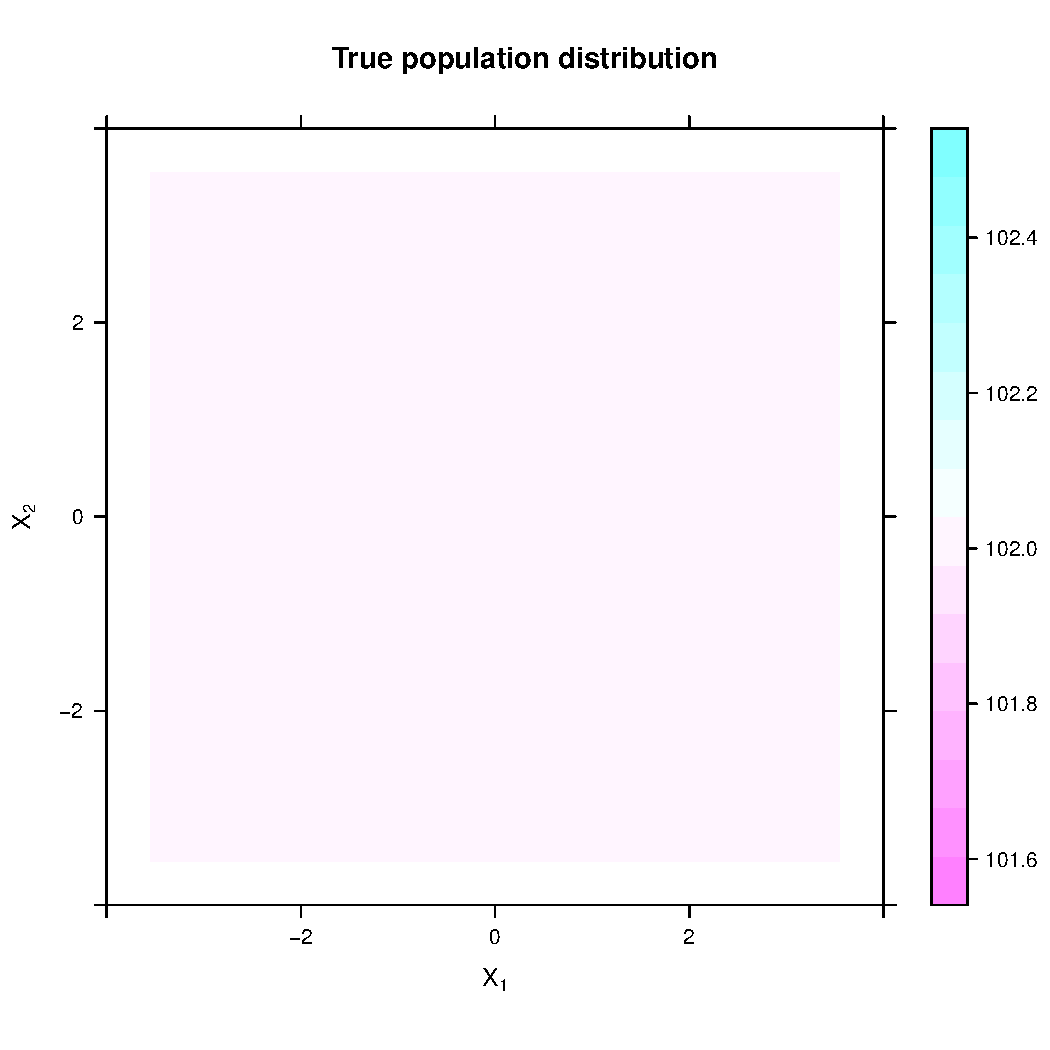
\includegraphics[width=\textwidth]{output/population-heatmap}
        \subcaption{Population distribution}
        \label{fig:cases_scatter:unif_100_1.0_1h:popdist}
    \end{subfigure}
    \begin{subfigure}[t]{0.32\textwidth}
        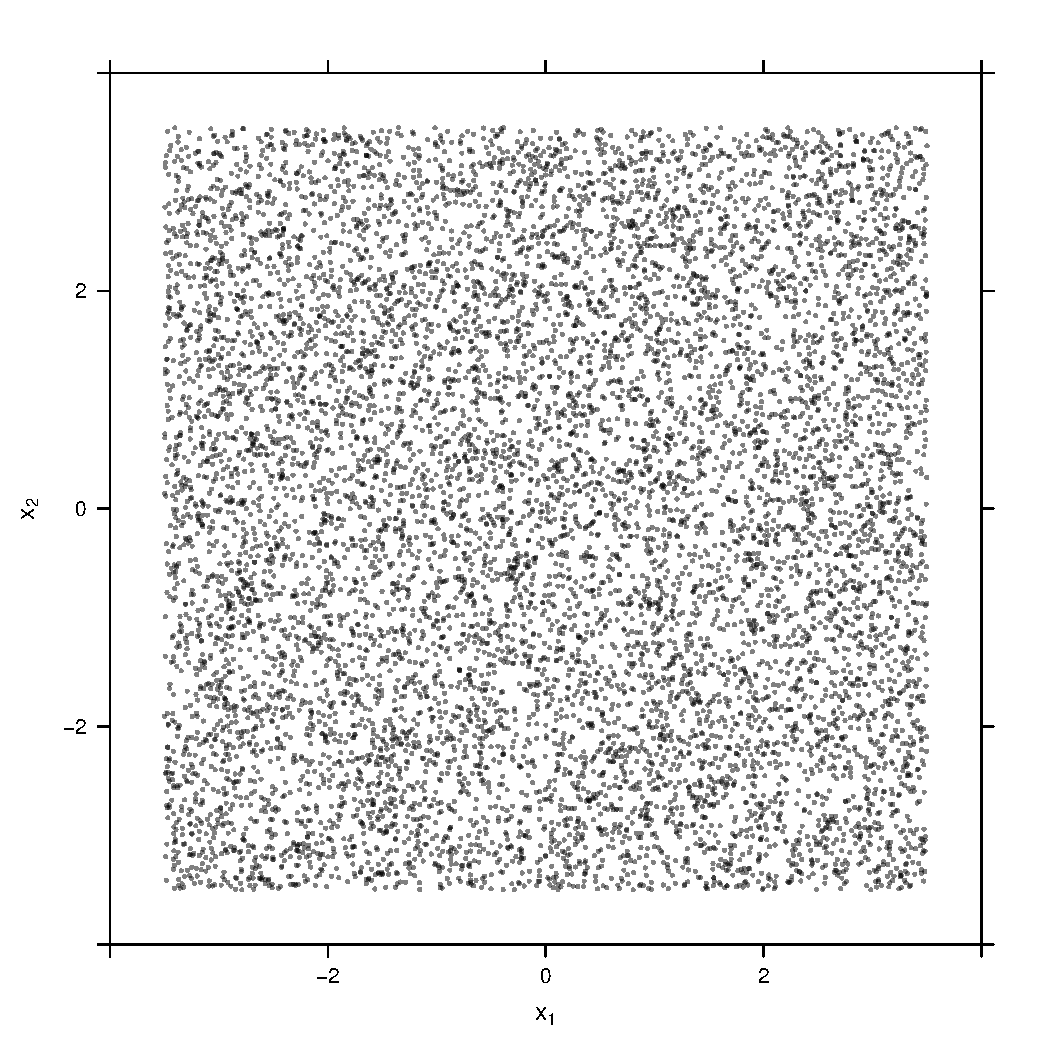
\includegraphics[width=\textwidth]{output/population-points}
        \subcaption{Population realization}
        \label{fig:cases_scatter:unif_100_1.0_1h:poppts}
    \end{subfigure}%
    \begin{subfigure}[t]{0.32\textwidth}
        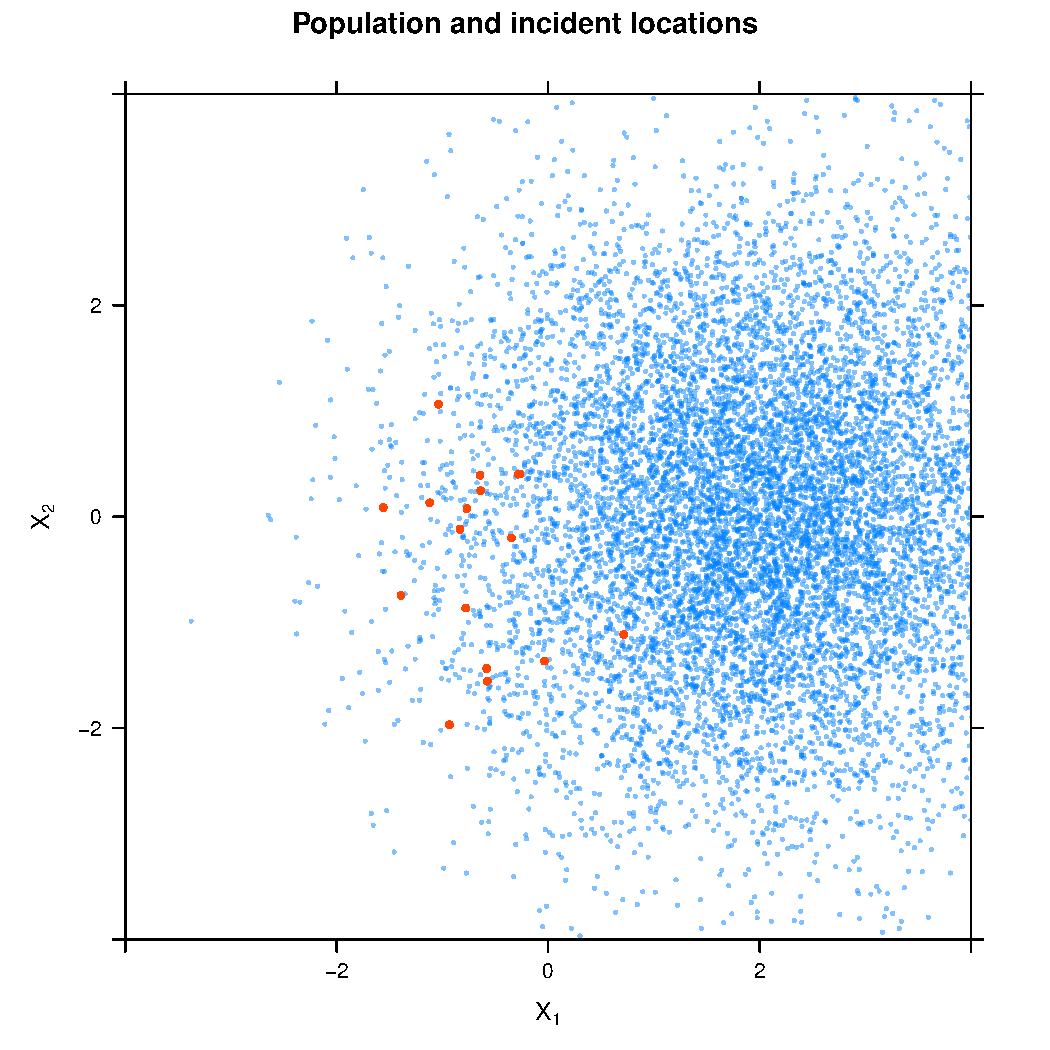
\includegraphics[width=\textwidth]{output/population_and_incidents_scatter}
        \subcaption{With incidents (triangles)}
        \label{fig:cases_scatter:unif_100_1.0_1h:incidentspts}
    \end{subfigure}%
    \caption[Example population and incidents: single-peak risk on uniform population]
        {Example population and incidents of one realization of single-peak risk of \glsentryname{factor} 100 with \glsentryname{spread} of 1.0 on a uniform population of 10,000.}
    \label{fig:cases_scatter:unif_100_1.0_1h}    
\end{figure}

%%%%%%%%%%%%%%%%%%%%%%%%%%%%%%%%%%%%%%%%%%%%%%%%%
% Example cases heat map - unif_100_1.0_1h
%%%%%%%%%%%%%%%%%%%%%%%%%%%%%%%%%%%%%%%%%%%%%%%%%
\begin{figure}[htbp]
    \centering
    \begin{subfigure}[t]{0.45\textwidth}
        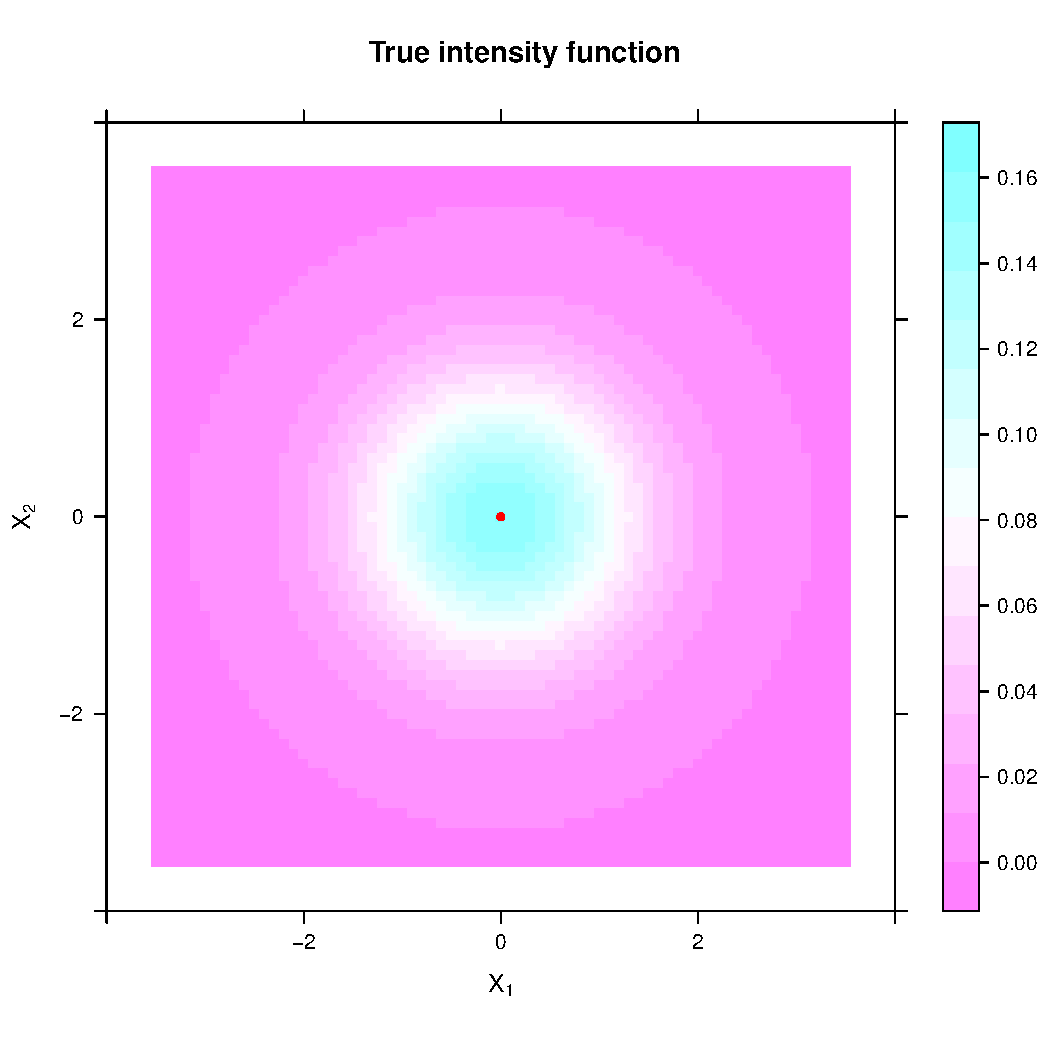
\includegraphics[width=\textwidth]{output/true_intensity_heatmap}
        \subcaption{True incident risk function}
        \label{fig:cases_heatmap:unif_100_1.0_1h:true}
    \end{subfigure}%
    \begin{subfigure}[t]{0.45\textwidth}
        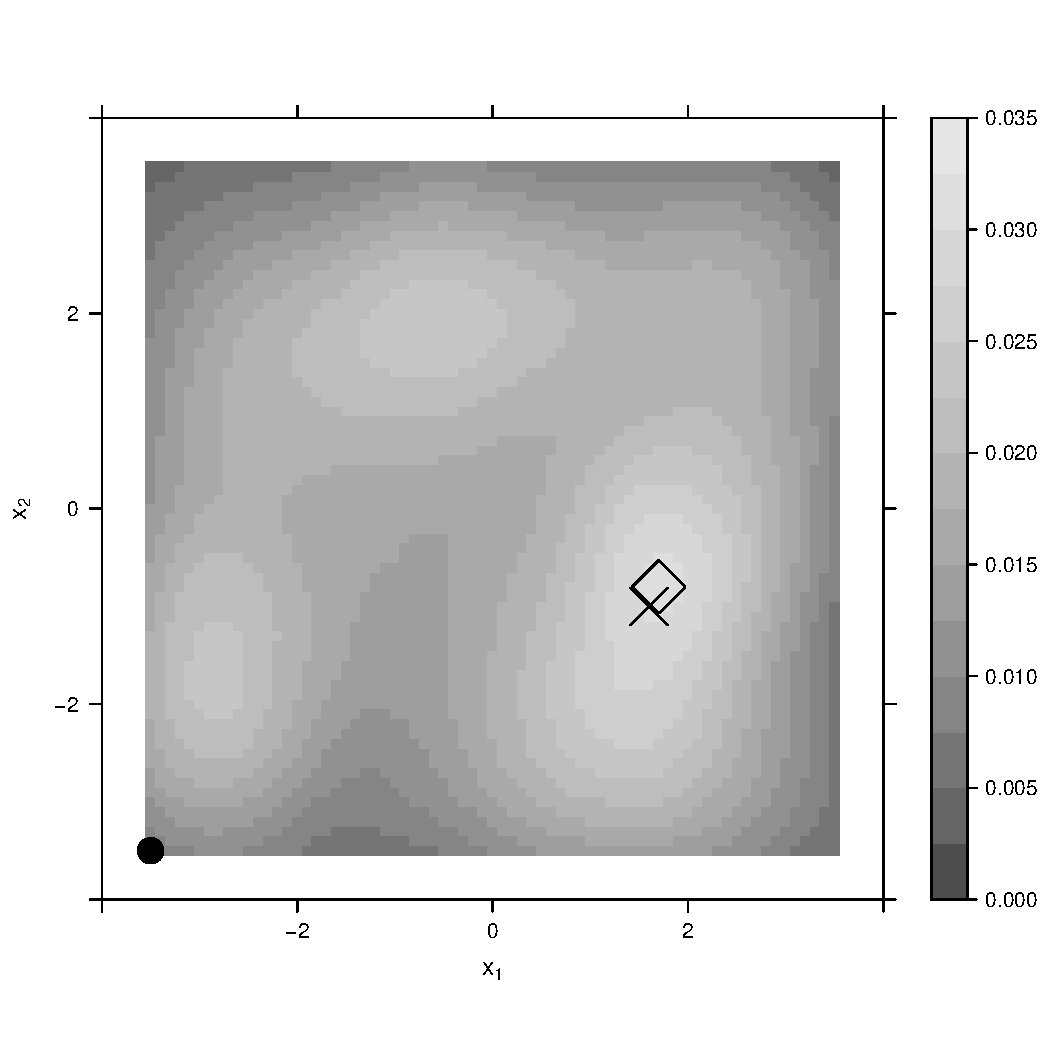
\includegraphics[width=\textwidth]{output/oracle_intensity_heatmap}
        \subcaption{Incident risk estimate using Oracle bandwidth}
        \label{fig:cases_heatmap:unif_100_1.0_1h:oracle}
    \end{subfigure}

    \begin{subfigure}[b]{0.45\textwidth}
        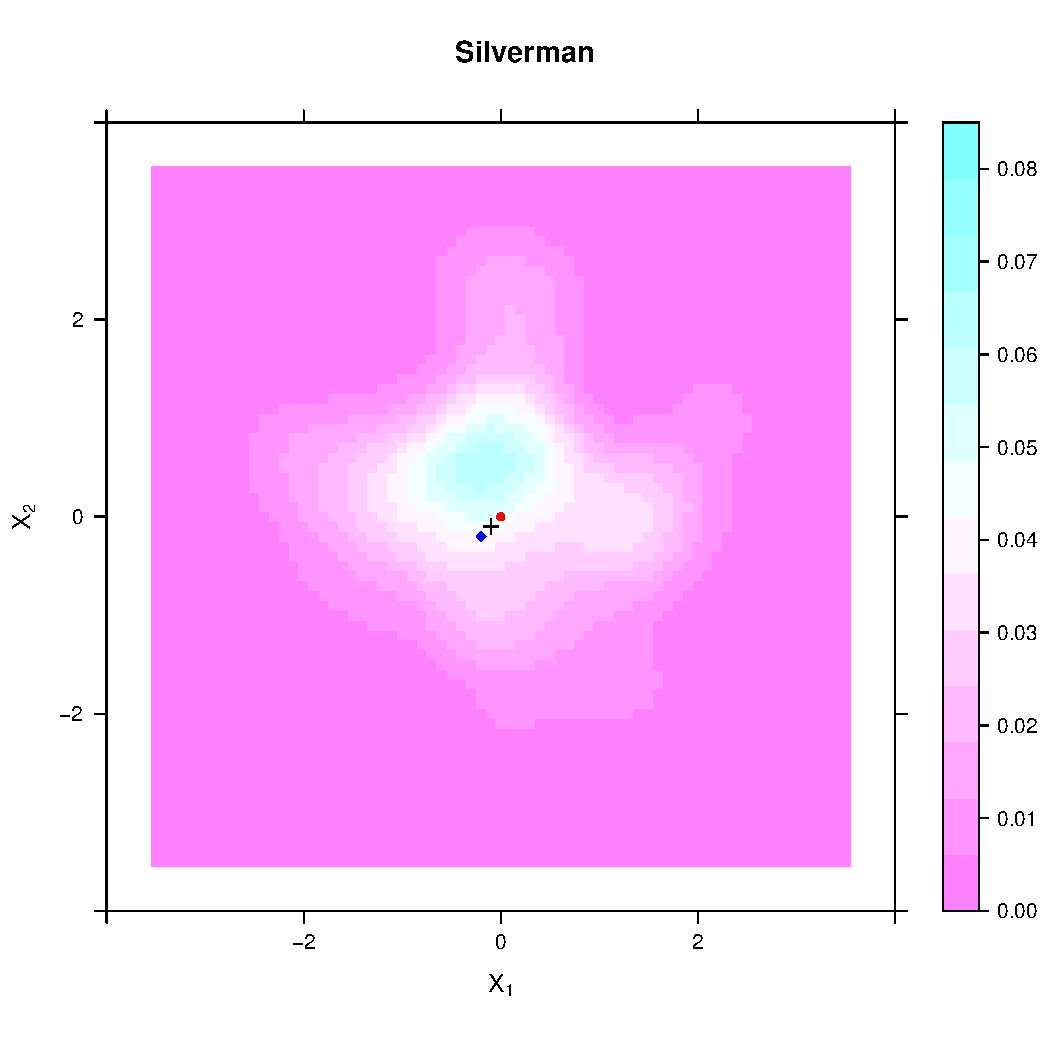
\includegraphics[width=\textwidth]{output/silverman_intensity_heatmap}
        \subcaption{Incident risk estimate using Silverman bandwidth}
        \label{fig:cases_heatmap:unif_100_1.0_1h:silverman}
    \end{subfigure}%
    \begin{subfigure}[b]{0.45\textwidth}
        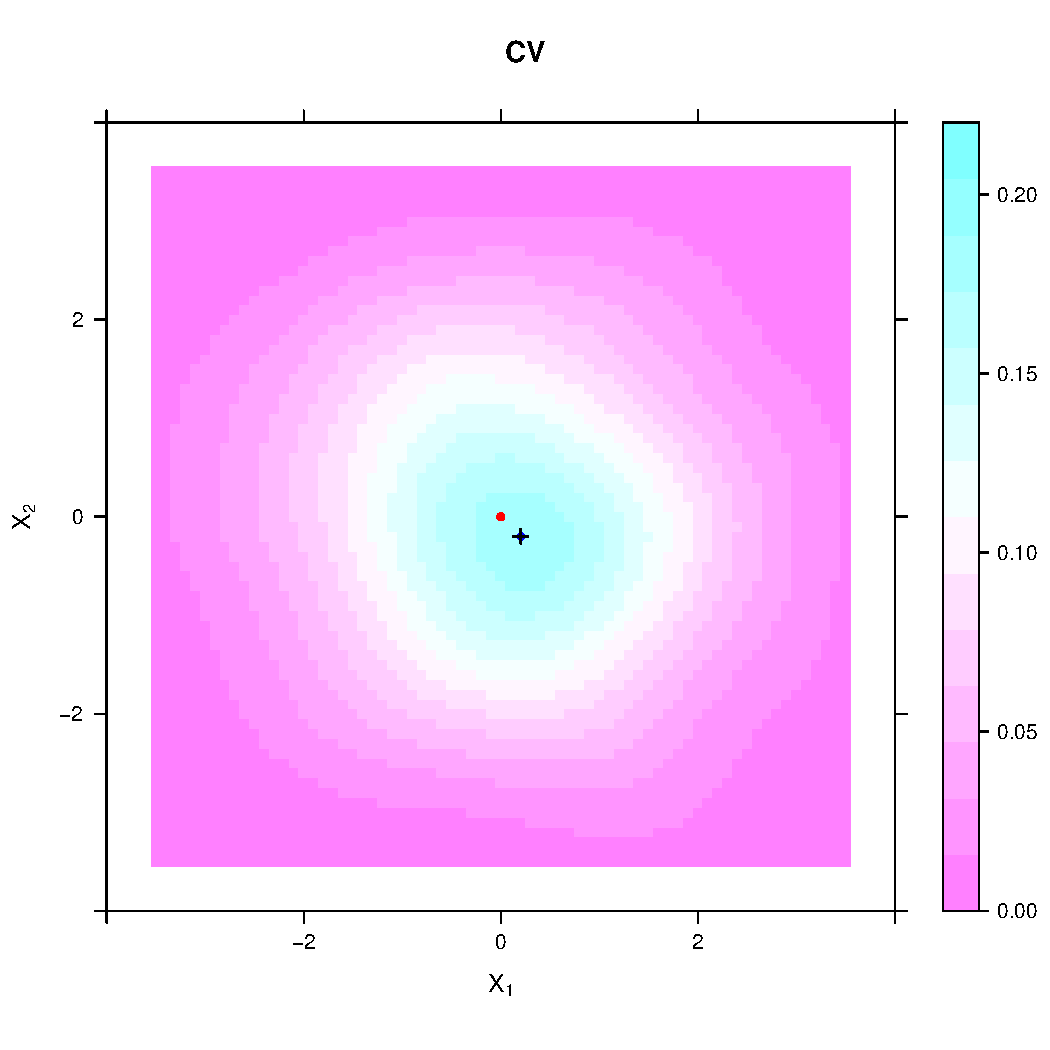
\includegraphics[width=\textwidth]{output/CV_intensity_heatmap}
        \subcaption{Incident risk estimate using Cross-validation bandwidth}
        \label{fig:cases_heatmap:unif_100_1.0_1h:cv}
    \end{subfigure}
    \caption[Example incidents: uniform incident risk on uniform population, 100 cases]
        {Example incidents: uniform incident risk on uniform population, 100 cases. The solid circles are the true peak. The diamonds are the peaks of the estimates. The crosses are the centroid peaks of the estimates.}
    \label{fig:cases_heatmap:unif_100_1.0_1h}
\end{figure}

In order to better understand the incident risk and the estimates,
we use a two-dimensional geographic heatmap of the study area \gls{W} to show a single simulation realization in
\Cref{fig:cases_heatmap:unif_100_1.0_1h}.
The lighter regions indicate a greater risk or estimated risk of an incident at that a point $\xvec$.
\Cref{fig:cases_heatmap:unif_100_1.0_1h:true} shows a heatmap of the true distribution function.
We see the \gls{dkd} estimates obtained using the \gls{oracle} in \subref{fig:cases_heatmap:unif_100_1.0_1h:oracle},
\gls{silverman} in \subref{fig:cases_heatmap:unif_100_1.0_1h:silverman} and \gls{cv} in \subref{fig:cases_heatmap:unif_100_1.0_1h:cv}.
The solid circles are the true peak.
The diamonds are the peaks of the estimates.
The crosses are the centroid peaks of the estimates.

%%%%%%%%%%%%%%%%%%%%%%%%%%%%%%%%%%%%%%%%%%%%%%%%%
% Mean errors - unif_100_1.0_1h
%%%%%%%%%%%%%%%%%%%%%%%%%%%%%%%%%%%%%%%%%%%%%%%%%
\begin{table}[htbp]
    \centering
    % latex table generated in R 3.4.2 by xtable 1.8-2 package
% Sat Feb 17 16:44:44 2018
\begin{tabular}{lrrr}
  \hline
 & Oracle & Silverman & CV \\ 
  \hline
MISE & 0.000053 & 0.000083 & 0.000080 \\ 
  Relative MISE & 0.002028 & 0.003195 & 0.003047 \\ 
  Normalized MISE & 0.000026 & 0.000042 & 0.000040 \\ 
  MIAE & 0.003914 & 0.004863 & 0.004653 \\ 
  Relative MIAE & 0.024227 & 0.030102 & 0.028802 \\ 
  Max Error & 0.033855 & 0.049415 & 0.045884 \\ 
  Peak bias & -0.016050 & 0.010816 & -0.002953 \\ 
  Relative Peak bias & -0.099339 & 0.066949 & -0.018278 \\ 
  Peak drift & 0.223424 & 0.357624 & 0.284159 \\ 
  Relative Peak drift & 0.031918 & 0.051089 & 0.040594 \\ 
  Centroid bias & -0.017140 & -0.000902 & -0.013918 \\ 
  Relative Centroid bias & -0.106087 & -0.005583 & -0.086149 \\ 
  Centroid drift & 0.149249 & 0.159867 & 0.152694 \\ 
  Relative Centroid drift & 0.021321 & 0.022838 & 0.021813 \\ 
   \hline
\end{tabular}

    \caption{Mean error rates for uniform population, single-peak risk with \glsentryname{spread} 1.0 of \glsentryname{factor} 100}
    \label{tab:errors:unif_100_1.0_1h}
\end{table}

\Cref{tab:errors:unif_100_1.0_1h} contains a summary of all of the measures of accuracy for this experiment.
We can see that for most measures, the \gls{oracle} selected bandwidth provides the best results.
Since the \gls{oracle} bandwidth is designed to approximate the \gls{mise}-optimal bandwidth \gls{h_opt},
this is not surprising.
However, in real world scenarios, the true function is unknown, and hence it is impossible to compute the \gls{oracle} bandwidth.
Therefore, we are interested in knowing how close the \gls{silverman} and \gls{cv} bandwidth selection methods can get to the \gls{oracle} for the different measures.
One exception is the \gls{peak bias}, which measures the difference between the maximum of the estimated risk and the maximum of the true risk (see \Cref{subsec:method:peak_bias}).
In this experiment, the \gls{silverman} and \gls{cv} bandwidths produced lower absolute \gls{peak bias} values than the \gls{oracle}. 
However, the \gls{oracle} and \gls{cv} bandwidths resulted in negative biases,
which is what we expected,
since the process of smoothing generally lowers high values (peaks) and raises low values.
The \gls{silverman} bandwidth, on the other hand, produced a positive value,
which may indicate under-smoothing.
This requires further study.

In \Cref{fig:ise:unif_100_1.0_1h}, we look at the distribution of the \gls{ise}.
As described in \Cref{subsec:method:mise},
the \gls{iae} gives a summary of the error of the estimate over all of \gls{W},
that penalizes higher error values.
In particular, we see that the relative and normalized \gls{ise} have similarly shaped distributions, although the scale is different.
We also observe that the distributions are skewed to the right,
indicating that for this simple setup,
the accuracy of the \gls{dkd} for a specific sample is more likely to be below the \gls{mise}.
Finally, we note that the estimates calculated with \gls{silverman} and \gls{cv}
selected bandwidths and their corresponding mean values had similar performance in \gls{ise}.

%%%%%%%%%%%%%%%%%%%%%%%%%%%%%%%%%%%%%%%%%%%%%%%%%
% ISE distribution - unif_100_1.0_1h
%%%%%%%%%%%%%%%%%%%%%%%%%%%%%%%%%%%%%%%%%%%%%%%%%
\begin{figure}[htbp]
    \centering
    \begin{subfigure}[b]{0.45\textwidth}
        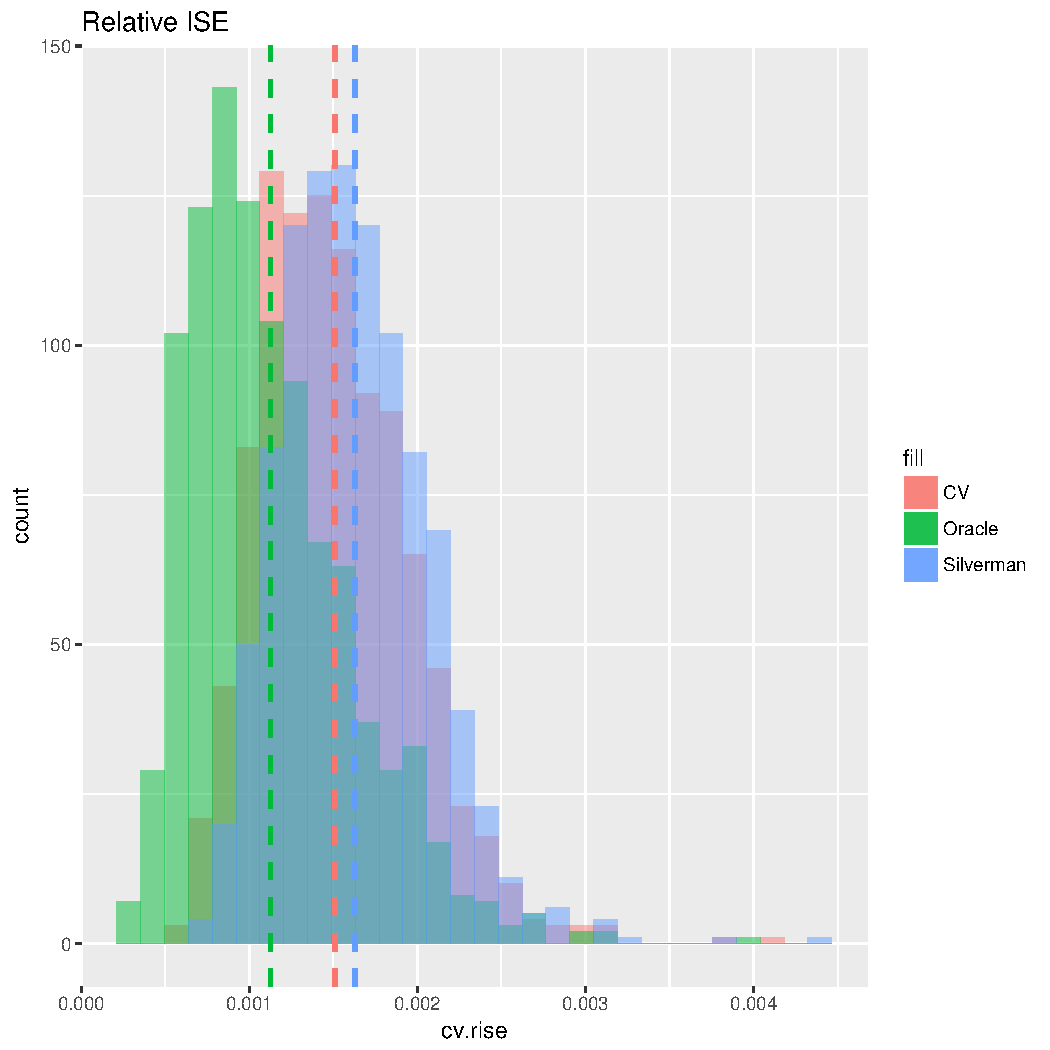
\includegraphics[width=\textwidth]{output/ise-relative-histogram}
        \subcaption{Relative \glsentryname{ise}}
    \end{subfigure}
    \begin{subfigure}[b]{0.45\textwidth}
        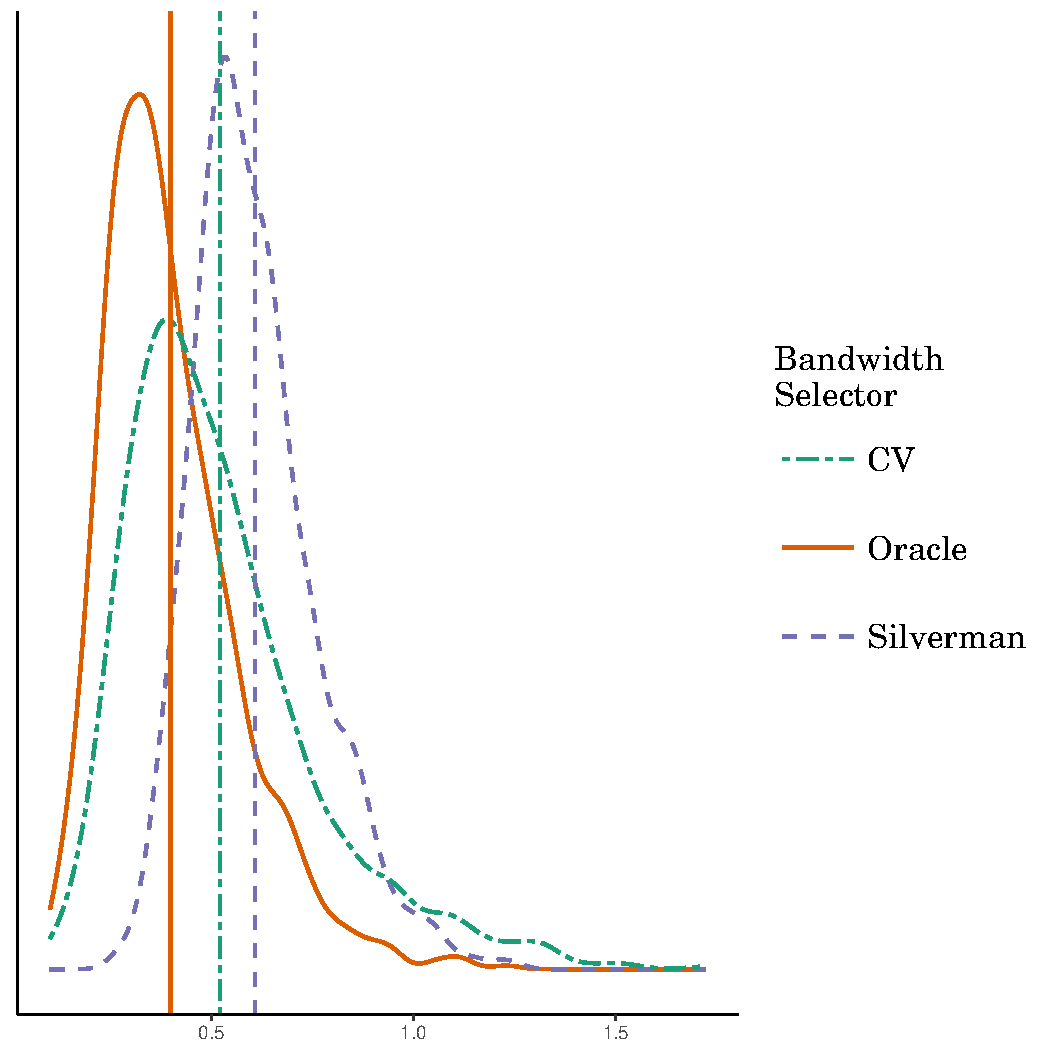
\includegraphics[width=\textwidth]{output/ise-normalized-histogram}
        \subcaption{Normalized \glsentryname{ise}}
    \end{subfigure}
    \caption[\glsentryname{ise}: Single-peak of 100 on uniform population]{\glsentryname{ise} density for a single-peak intensity with \glsentryname{spread} of 1.0 and \glsentryname{factor} of 100 on a uniform population. Vertical lines indicate the estimated \glsentryname{mise} of the simulations. \glsentryname{nmise} values are multiplied by $10^9$.}
    \label{fig:ise:unif_100_1.0_1h}
\end{figure}

%%%%%%%%%%%%%%%%%%%%%%%%%%%%%%%%%%%%%%%%%%%%%%%%%
% IAE distribution - unif_100_1.0_1h
%%%%%%%%%%%%%%%%%%%%%%%%%%%%%%%%%%%%%%%%%%%%%%%%%
\begin{figure}[htbp]
    \centering
    \begin{subfigure}[b]{0.45\textwidth}
        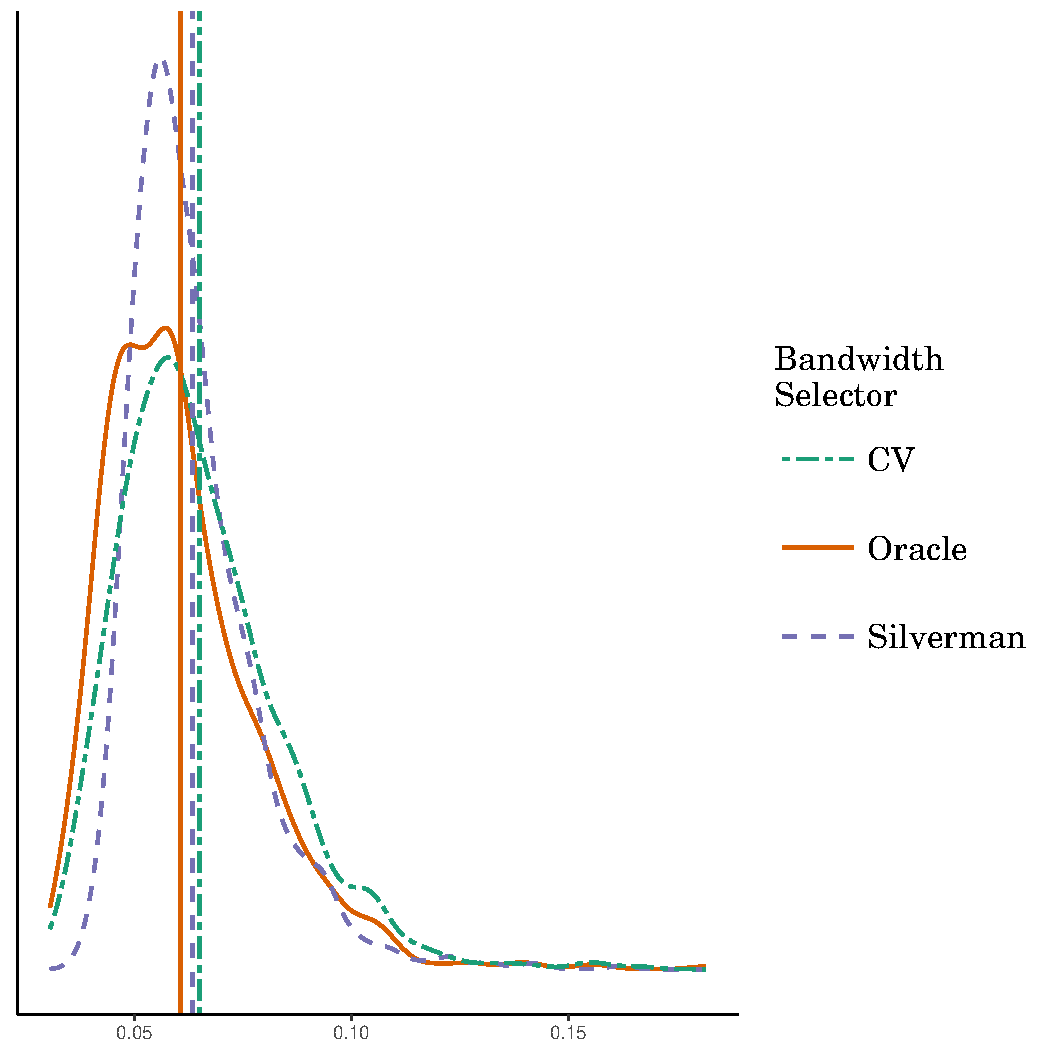
\includegraphics[width=\textwidth]{output/iae-relative-histogram}
        \subcaption{Relative \glsentryname{iae}}
    \end{subfigure}
    \begin{subfigure}[b]{0.45\textwidth}
        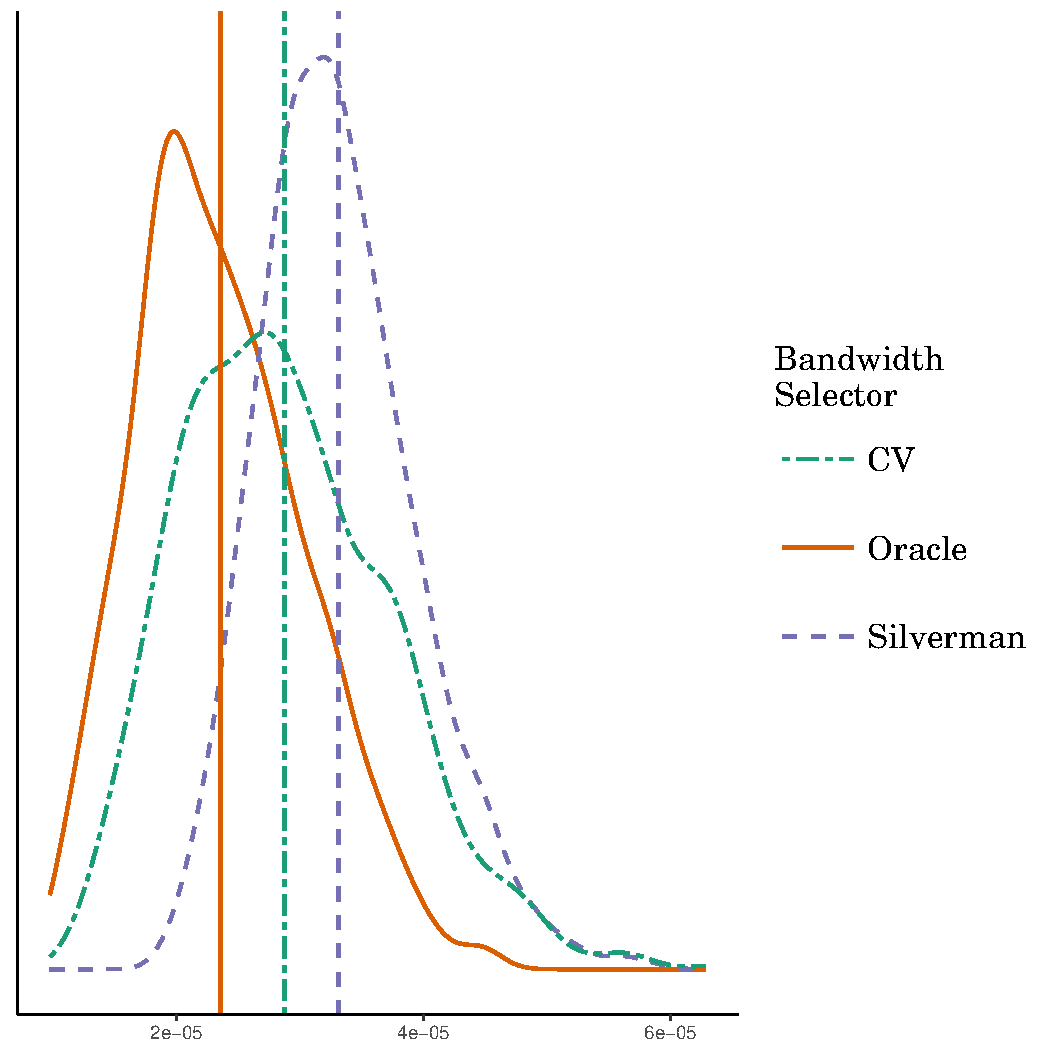
\includegraphics[width=\textwidth]{output/iae-normalized-histogram}
        \subcaption{Normalized \glsentryname{iae}}
    \end{subfigure}
    \caption[\glsentryname{iae}: Single-peak of 100 on uniform population]{\glsentryname{iae} density for a single-peak intensity with \glsentryname{spread} of 1.0 and \glsentryname{factor} of 100 on a uniform population. Vertical lines indicate the estimated \glsentryname{miae} of the simulations.}
    \label{fig:iae:unif_100_1.0_1h}
\end{figure}

%%%%%%%%%%%%%%%%%%%%%%%%%%%%%%%%%%%%%%%%%%%%%%%%%
% Max error distribution - unif_100_1.0_1h
%%%%%%%%%%%%%%%%%%%%%%%%%%%%%%%%%%%%%%%%%%%%%%%%%
\begin{figure}[htbp]
    \centering
    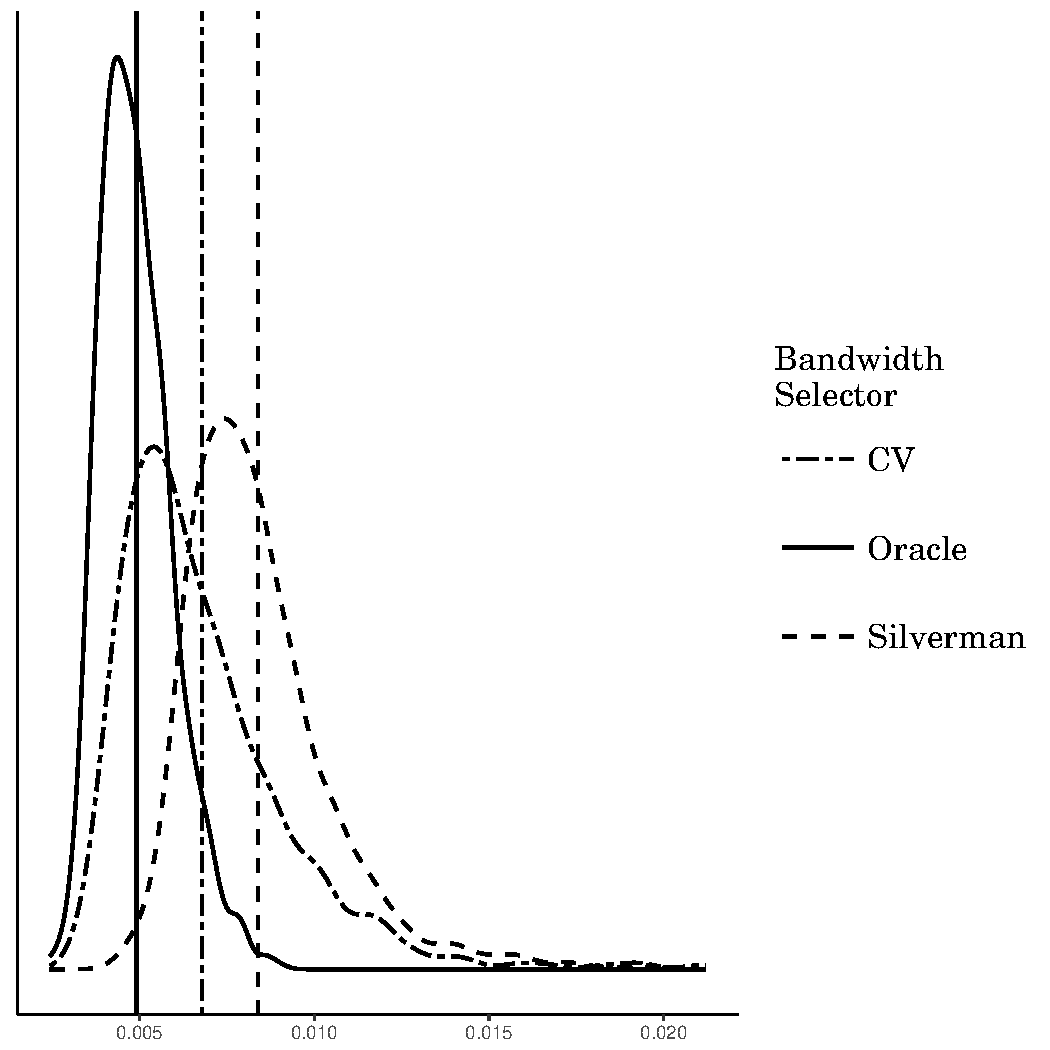
\includegraphics[width=0.45\textwidth]{output/maxerr-histogram}
    \caption[\glsentryname{supremum error}: Single-peak of 100 on uniform population]{\glsentryname{supremum error} density for a single-peak intensity with \glsentryname{spread} of 1.0 and \glsentryname{factor} of 100 on a uniform population. Vertical lines indicate the estimated mean \glsentryname{supremum error} of the simulations.}
    \label{fig:maxerr:unif_100_1.0_1h}
\end{figure}

\Cref{fig:ise:unif_100_1.0_1h} shows the relative and normalized distributions of the \gls{iae}.
As described in \Cref{subsec:method:miae},
the \gls{iae} gives a summary of the error of the estimate over all of \gls{W},
giving equal weight to all error values.
Once again, the normalized and relative error measures have similar distributions.
The \gls{oracle} bandwidth selection technique is still notably more accurate when comparing with \gls{iae} than with \gls{ise}.
However, for \gls{iae} we see that \gls{cv} bandwidth selection results in a wider distribution than with \gls{silverman}.

In \Cref{fig:maxerr:unif_100_1.0_1h}, we look at the distribution of the \gls{supremum error}.
As described in \Cref{subsec:method:sup_error},
the \gls{supremum error} is the worst-case error of the estimate on \gls{W}.
We observe that the distributions are once again skewed to the right,
indicating that for this simple setup,
the worst-case accuracy of the \gls{dkd} for a specific sample is more likely to be below the average \gls{supremum error}.
Finally, we note that the estimates calculated with \gls{silverman} and \gls{cv}
selected bandwidths and their corresponding mean values had similar performance in \gls{supremum error}.


%%%%%%%%%%%%%%%%%%%%%%%%%%%%%%%%%%%%%%%%%%%%%%%%%
% Peaks - unif_100_1.0_1h
%%%%%%%%%%%%%%%%%%%%%%%%%%%%%%%%%%%%%%%%%%%%%%%%%
\begin{figure}[htbp]
    \centering
    \begin{subfigure}[b]{0.45\textwidth}
        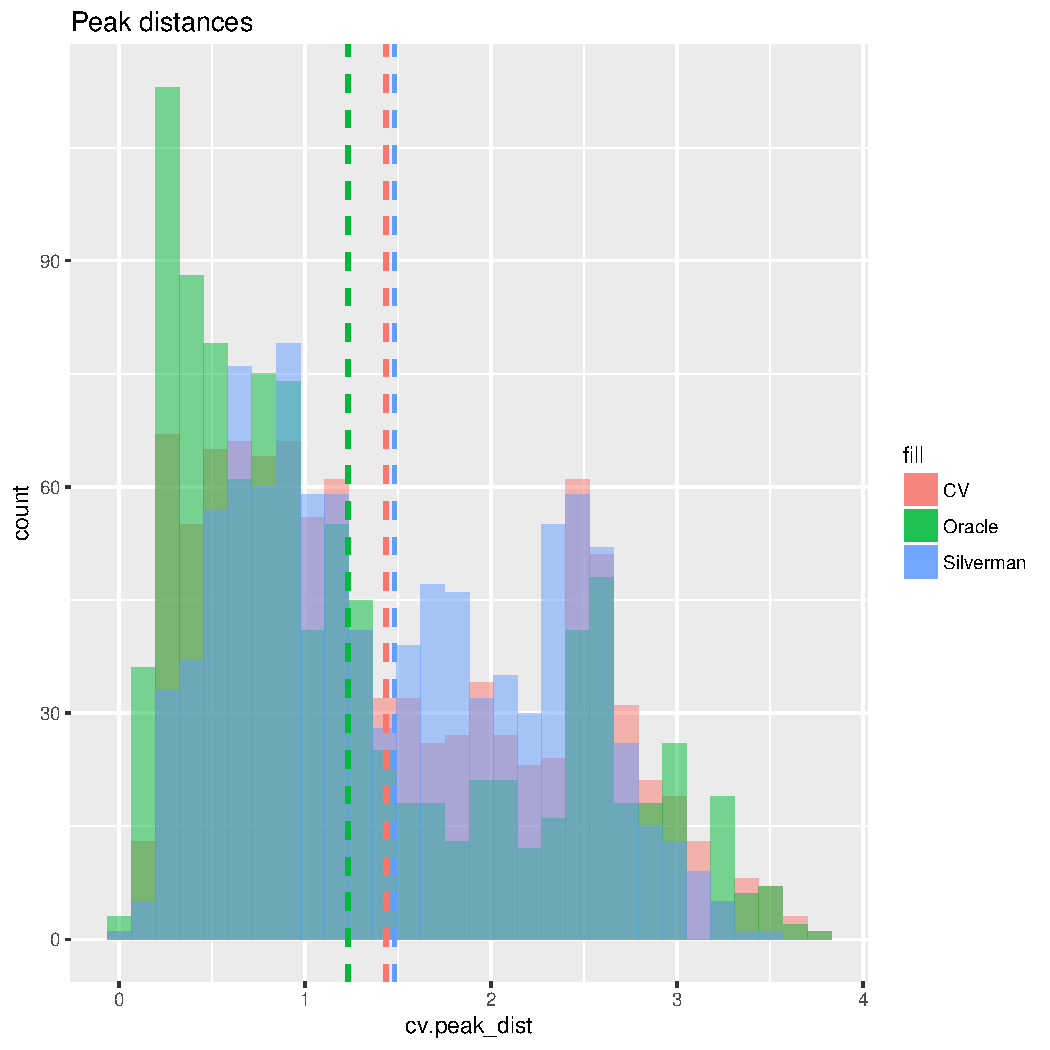
\includegraphics[width=\textwidth]{output/peak-dist-histogram}
        \subcaption{Peak distance from truth}
        \label{fig:peaks:unif_100_1.0_1h:dist}
    \end{subfigure}
    \begin{subfigure}[b]{0.45\textwidth}
        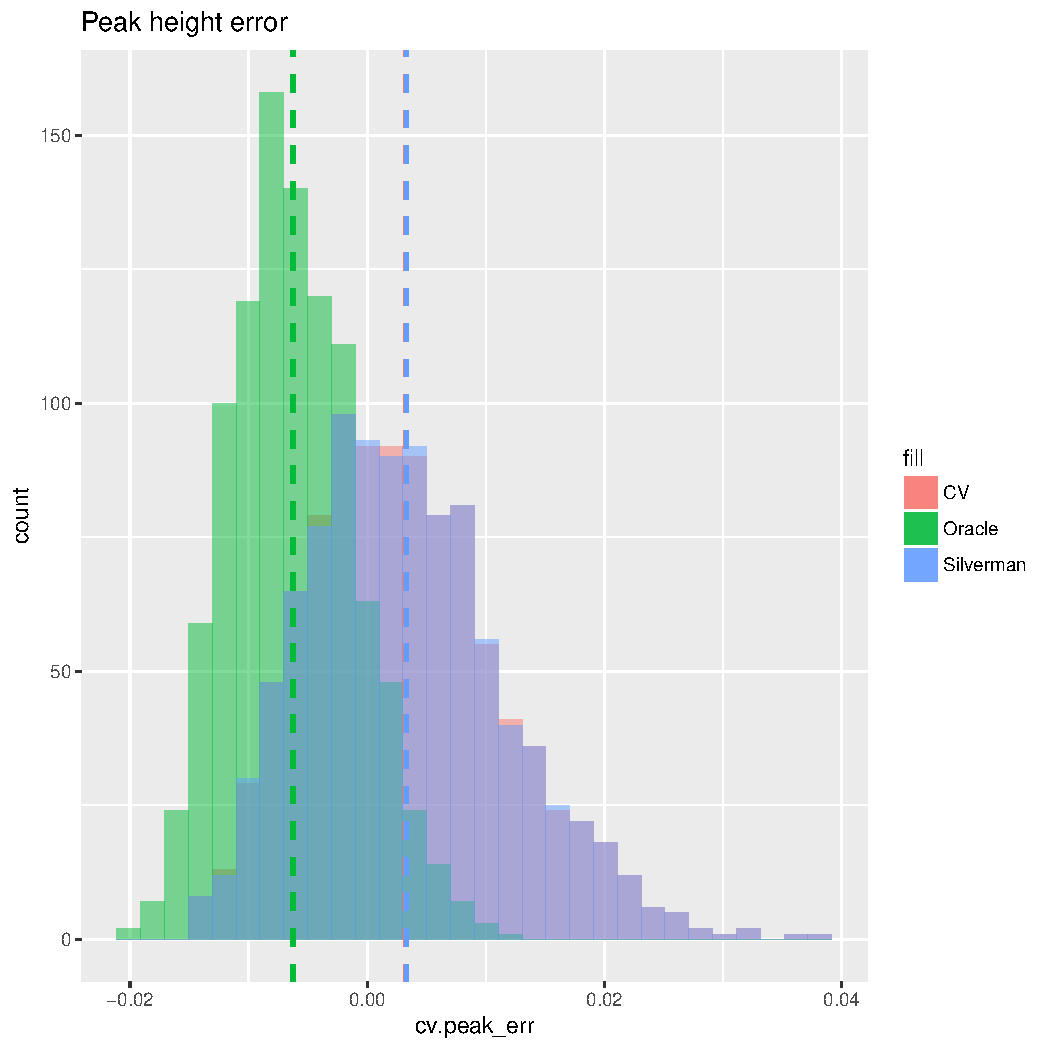
\includegraphics[width=\textwidth]{output/peak-height-histogram}
        \subcaption{Peak height error}
        \label{fig:peaks:unif_100_1.0_1h:height}
    \end{subfigure}
    \caption[Peak accuracy: Single-peak of 100 on uniform population]{Peak accuracy measure densities for a single-peak intensity with \glsentryname{spread} of 1.0 and \glsentryname{factor} of 100 on a uniform population. Vertical lines indicate the mean values of the simulations.}
    \label{fig:peaks:unif_100_1.0_1h}
\end{figure}

%%%%%%%%%%%%%%%%%%%%%%%%%%%%%%%%%%%%%%%%%%%%%%%%%
% Centroids - unif_100_1.0_1h
%%%%%%%%%%%%%%%%%%%%%%%%%%%%%%%%%%%%%%%%%%%%%%%%%
\begin{figure}[htbp]
    \centering
    \begin{subfigure}[b]{0.45\textwidth}
        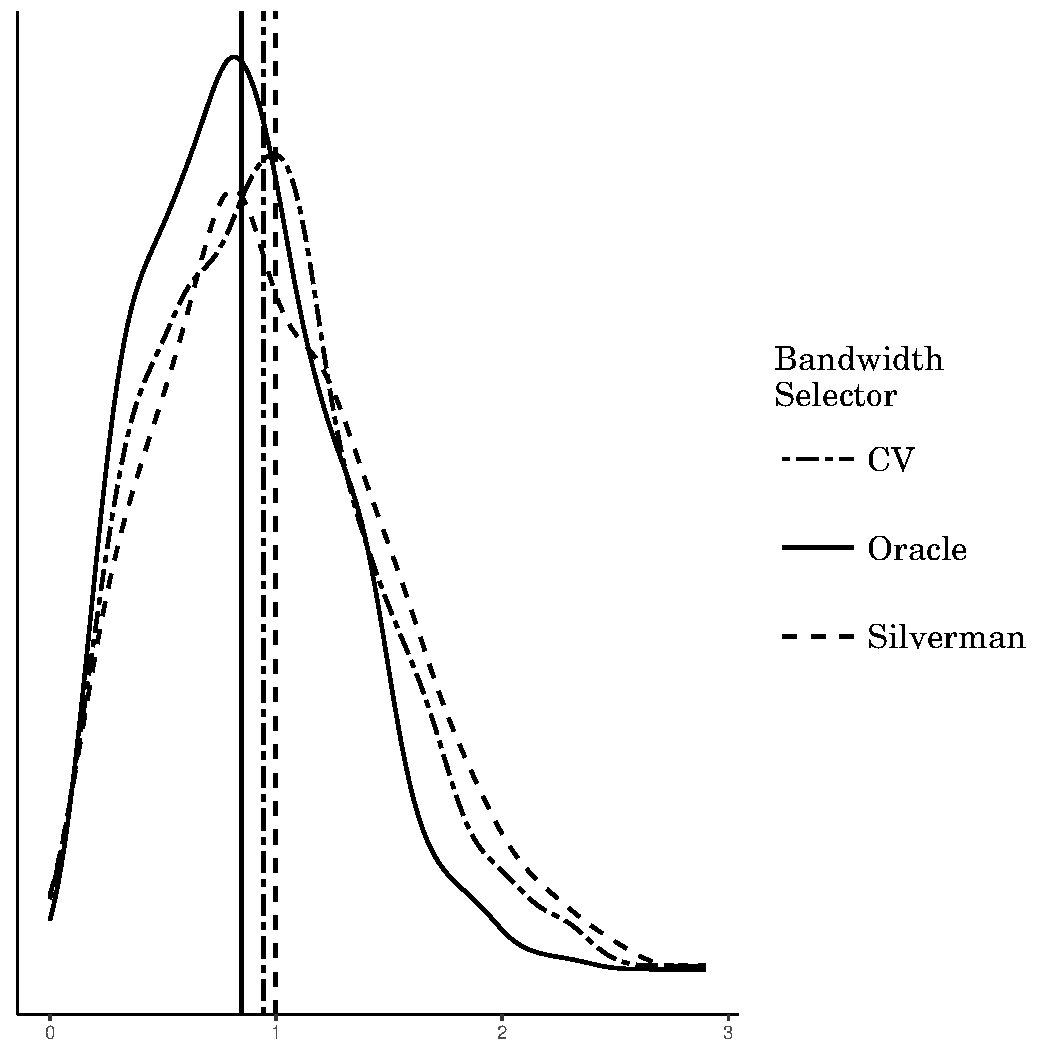
\includegraphics[width=\textwidth]{output/centroid-dist-histogram}
        \subcaption{Centroid peak distance from truth}
    \end{subfigure}
    \begin{subfigure}[b]{0.45\textwidth}
        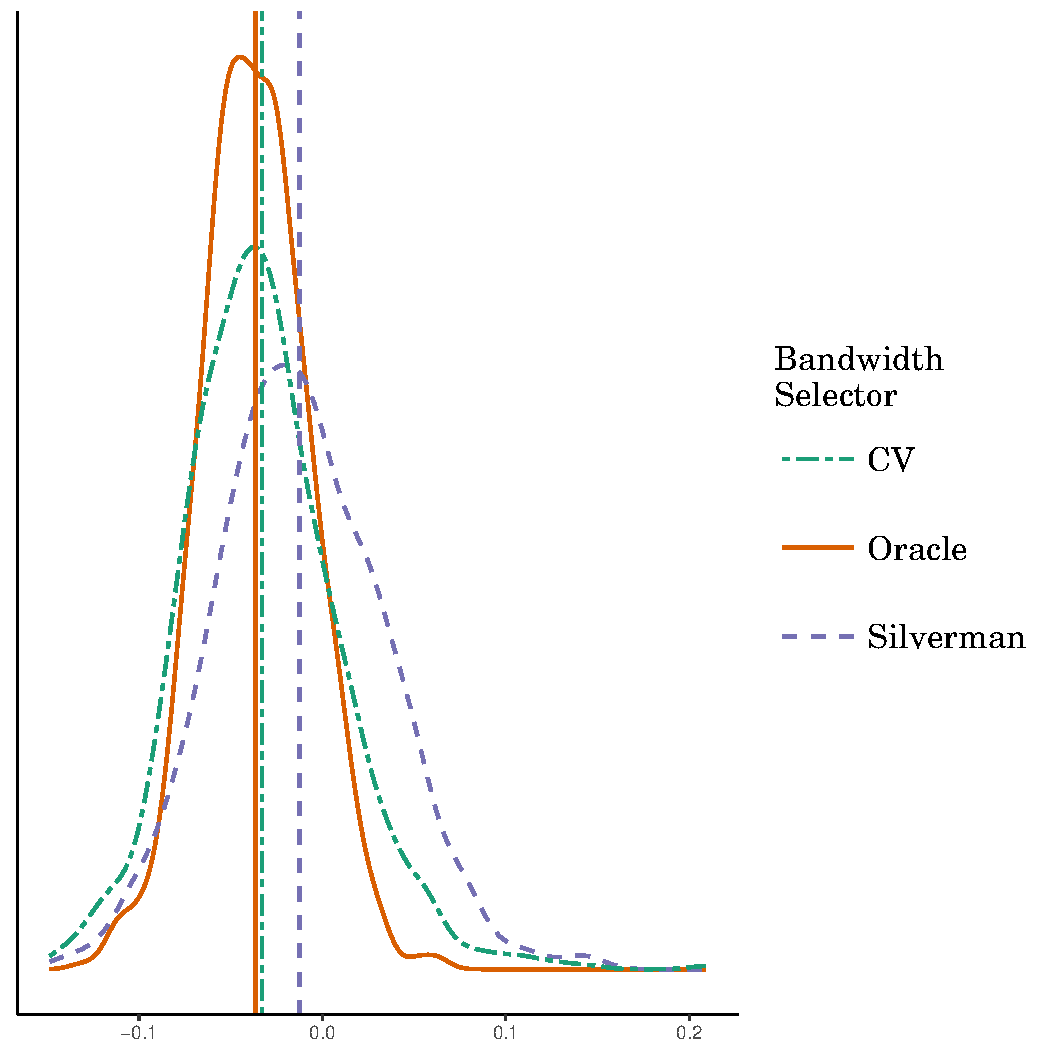
\includegraphics[width=\textwidth]{output/centroid-height-histogram}
        \subcaption{Centroid peak height error}
    \end{subfigure}
    \caption[Centroid accuracy: Single-peak of 100 on uniform population]{Peak accuracy measures densities sing centroid technique for a single-peak intensity with \glsentryname{spread} of 1.0 and \glsentryname{factor} of 100 on a uniform population. Vertical lines indicate the mean values of the simulations.}
    \label{fig:centroids:unif_100_1.0_1h}
\end{figure}

For both of the peak distance errors (\Cref{fig:peaks:unif_100_1.0_1h:dist}) and peak height errors (\Cref{fig:peaks:unif_100_1.0_1h:height}) of this experiment,
we see the \gls{cv} bandwidth selection outperforms the \gls{silverman} rule of thumb, and that the \gls{oracle} seems to outperform them both.
In fact, the \gls{peak bias}, which we estimate using the mean \gls{peak error},
is positive for \gls{silverman}.
This indicates a tendency towards under-smoothing.
We note that all three of bandwidth selection techniques are designed to minimize \gls{mise}.
We also note the multi-modal peak distance distributions.
We believe this is an artifact of the experimental design,
since our estimate of the peak will always be at one of a fixed, discrete number of points on a grid in the study area.

In \Cref{fig:centroids:unif_100_1.0_1h} we see the distributions of \gls{peak error} and \gls{peak drift} using the centroid estimation technique.
We note that the scales of both types of error are markedly improved.
That is, the centroid technique improves both the estimated location and estimated height of the peak.

%%%%%%%%%%%%%%%%%%%%%%%%%%%%%%%%%%%%%%%%%%%%%%%%%
% Bandwidths - unif_100_1.0_1h
%%%%%%%%%%%%%%%%%%%%%%%%%%%%%%%%%%%%%%%%%%%%%%%%%
\begin{figure}[htbp]
    \centering
    \begin{subfigure}[t]{0.45\textwidth}
        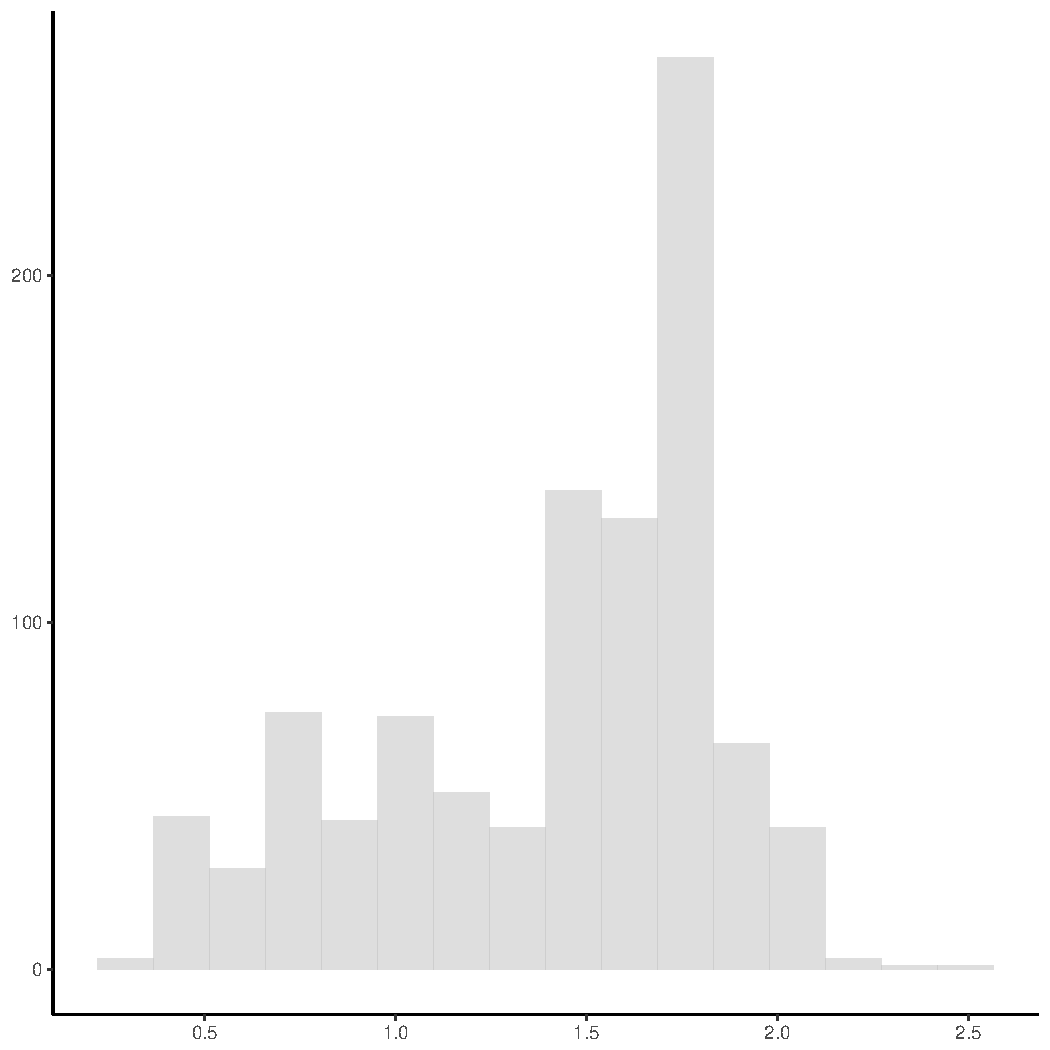
\includegraphics[width=\textwidth]{output/bandwidths-x1}
        \subcaption{CV Bandwidths - $x_1$}
        \label{fig:bandwidths:unif_100_1.0_1h:x1}
    \end{subfigure}
    \begin{subfigure}[t]{0.45\textwidth}
        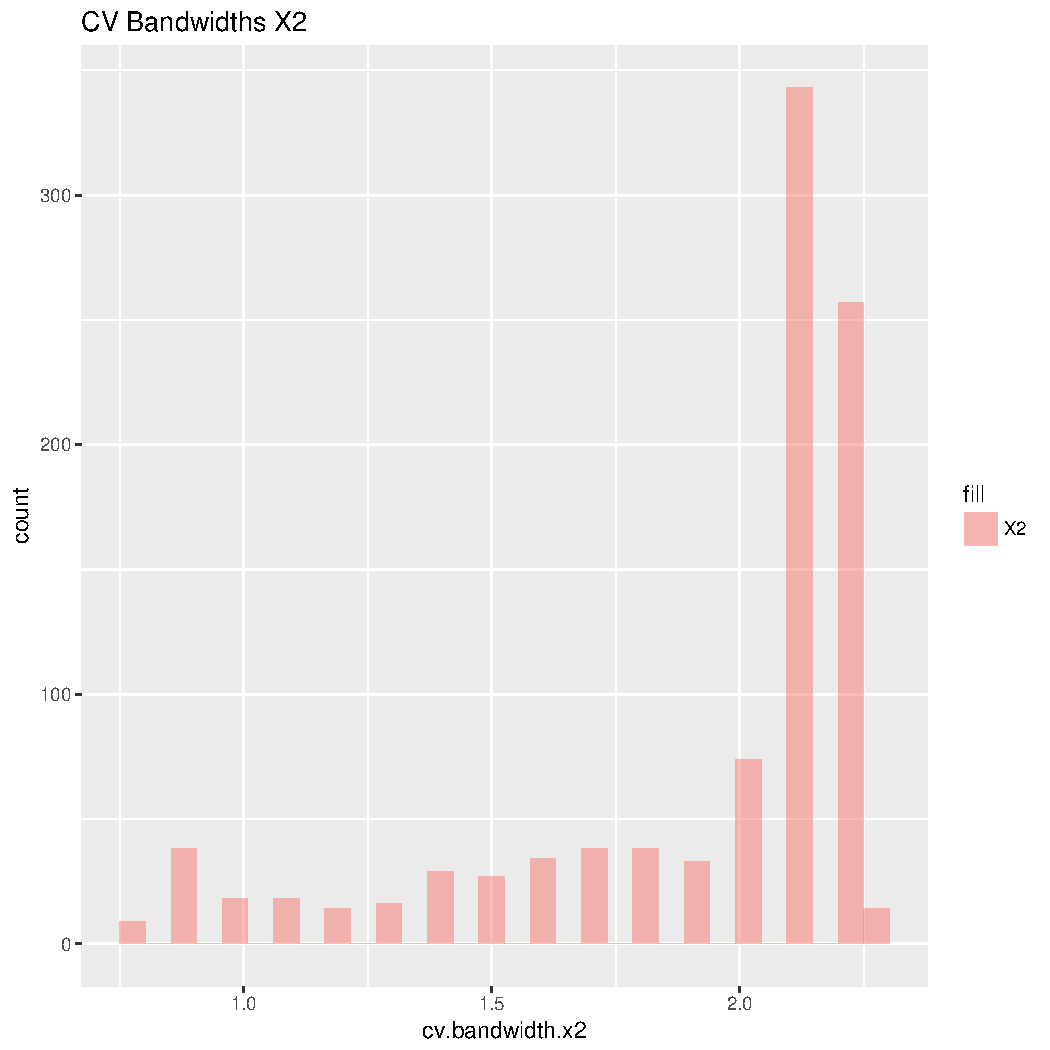
\includegraphics[width=\textwidth]{output/bandwidths-x2}
        \subcaption{CV Bandwidths - $x_2$}
        \label{fig:bandwidths:unif_100_1.0_1h:x2}
    \end{subfigure}

    \begin{subfigure}[t]{0.45\textwidth}
        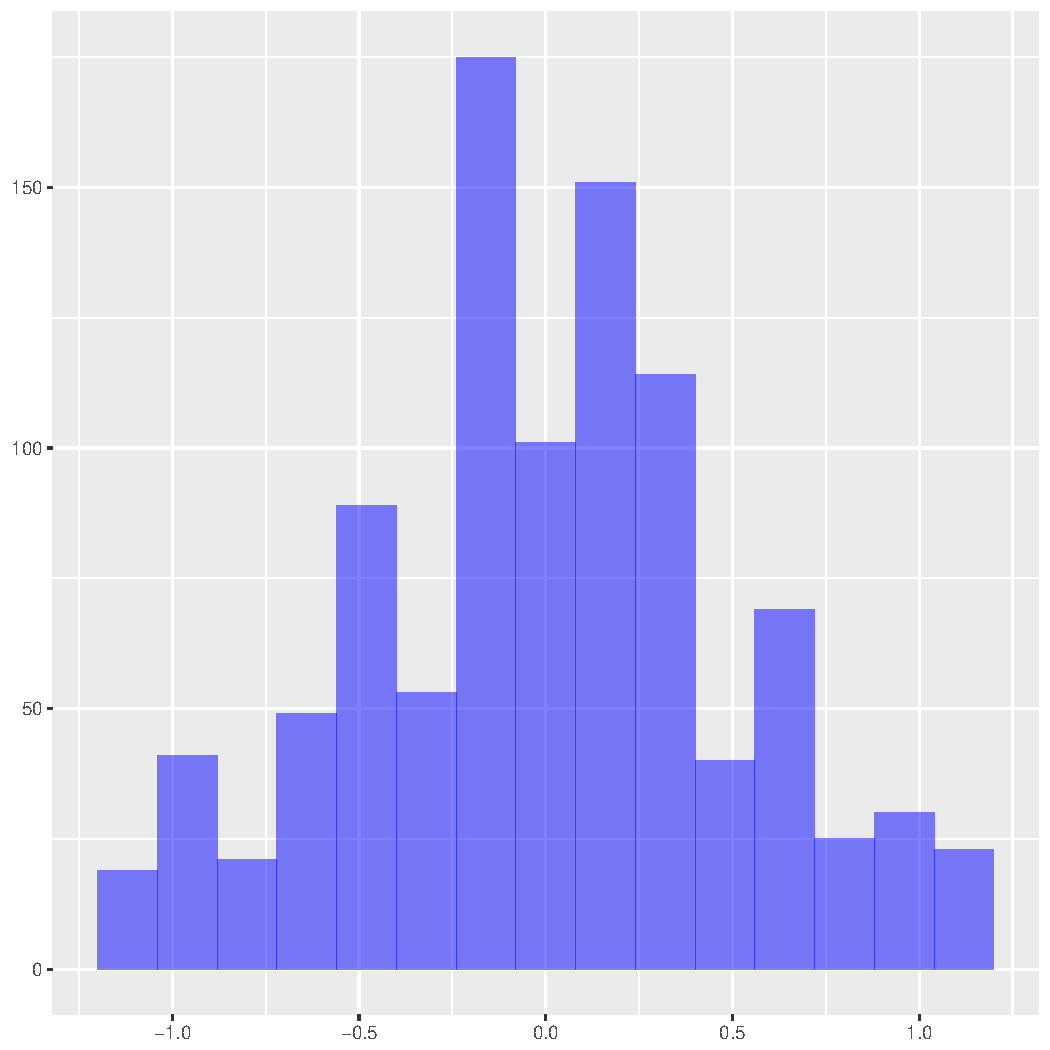
\includegraphics[width=\textwidth]{output/bandwidths-difference}
        \subcaption{Difference between $x_1$ and $x_2$ bandwidths}
        \label{fig:bandwidths:unif_100_1.0_1h:diff}
    \end{subfigure}
    \begin{subfigure}[t]{0.45\textwidth}
        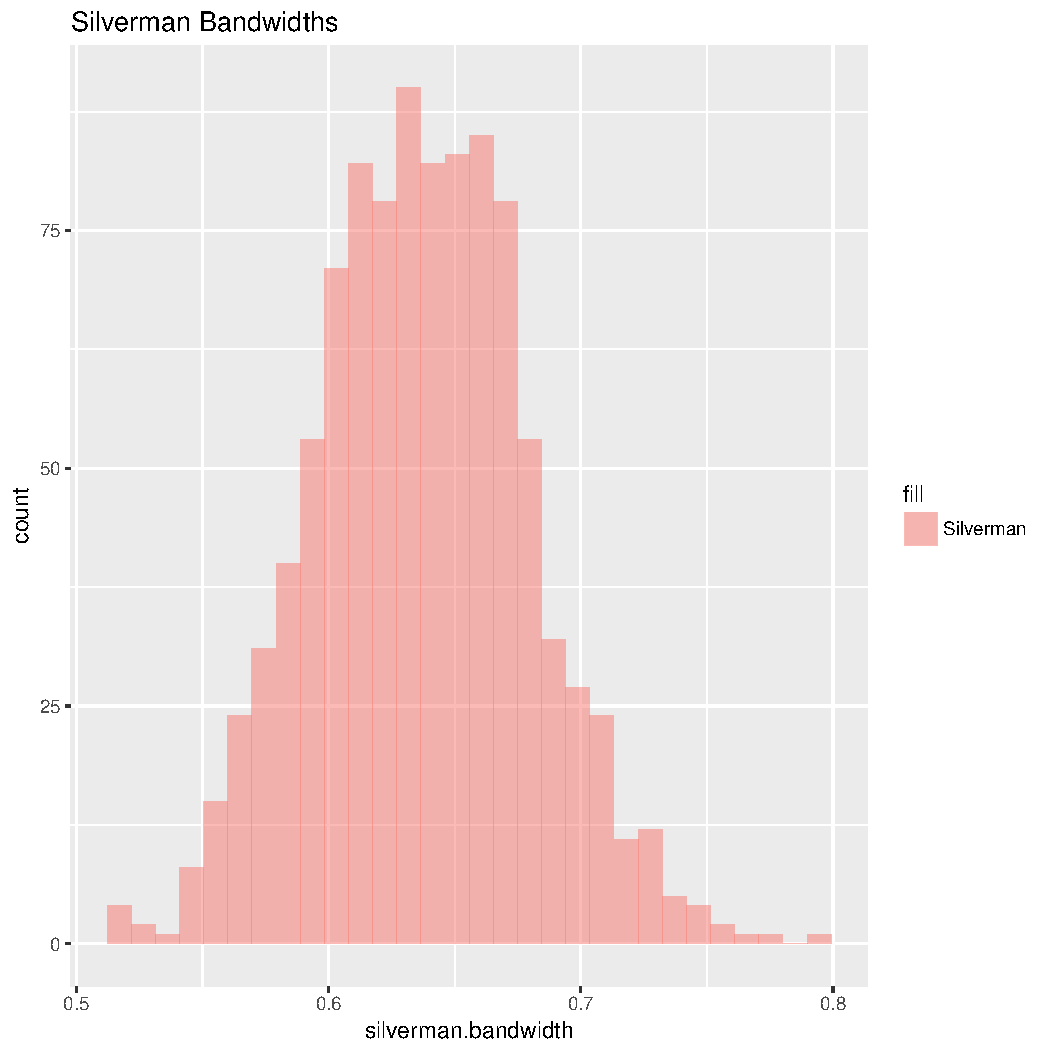
\includegraphics[width=\textwidth]{output/bandwidths-silverman}
        \subcaption{Silverman Bandwidths}
        \label{fig:bandwidths:unif_100_1.0_1h:silverman}
    \end{subfigure}
    \caption[Bandwidths: Single-peak of 100 on uniform population]{\glsentryname{cv} bandwidths: $x_1$, $x_2$ and difference and \glsentryname{silverman} bandwidth histograms for  a single-peak intensity with \glsentryname{spread} of 1.0 and \glsentryname{factor} of 100 on a uniform population}
    \label{fig:bandwidths:unif_100_1.0_1h}
\end{figure}

The bandwidths selected by \gls{cv} were allowed to vary in the $x_1$ and $x_2$ directions.
In \Cref{fig:bandwidths:unif_100_1.0_1h:x1,fig:bandwidths:unif_100_1.0_1h:x2} we see that the distributions of these bandwidths observed in this experiment are quite similar.
Since the true \gls{risk} function is invariant under a change of coordinates,
this is the behavior that we expect.
\Cref{fig:bandwidths:unif_100_1.0_1h:diff} shows that the $x_1$ and $x_2$ coordinate distributions often differ significantly in the individual realizations.
This is due to the randomness of the locations of the \glspl{incident},
which can cause the observed distribution of the points to vary between realizations.
The distribution of the \gls{silverman} selected bandwidths is much more symmetric, and has a lower mean value (\Cref{fig:bandwidths:unif_100_1.0_1h:silverman}).
This results in a slightly under-smoothed \gls{silverman} estimate.

% Restore graphics and input path
\setpath{}

%%%%%%%%%%%%%%%%%%%%%%%%%%%%%%%%%%%%%%%%%%%%%%%%%%%%%%%%%%%%%%%%%%%%%%%%%%%%%%
%%
%% Section: Effect of number of incidents with fixed population
%%
%%%%%%%%%%%%%%%%%%%%%%%%%%%%%%%%%%%%%%%%%%%%%%%%%%%%%%%%%%%%%%%%%%%%%%%%%%%%%%
\section[Effect of number of incidents with fixed population]
    {Effect of \glsentryname{factor} for a fixed, uniform population of 10,000 and single peak with \glsentryname{spread} 1.0}
\label{sec:results:number_of_incidents}

%%%%%%%%%%%%%%%%%%%%%%%%%%%%%%%%%%%%%%%%%%%%%%%%%
% Parameter table - expected number of incidents
%%%%%%%%%%%%%%%%%%%%%%%%%%%%%%%%%%%%%%%%%%%%%%%%%
\begin{table}[htbp]
    \centering
    \begin{tabular}{ll}
        \toprule
        Parameter & Value \\
        \midrule
        Population size & 10,000 \\
        Population \glsentryname{spread} & uniform \\
        Population center & uniform \\
        \Glsentryname{factor} & 50, 100, 200, 500, 1,000 \\
        Incident \glsentryname{spread} & 1.0 \\
        Incident center & (0,0) \\
        \bottomrule
    \end{tabular}
    \caption[Effect of \glsentryname{factor} with fixed population]
        {Experimental parameter values varying \glsentryname{factor} for a fixed, uniform population of 10,000 and single peak with spread 1.0}
    \label{tab:params:results:number_of_incidents}
\end{table}

In this section we examine and compare the results of five experiments in which we vary the \glspl{factor}
of a single-peak risk function.
The unknown information that one is trying to discover, is the risk of a person catching a specific disease over a defined time period.
This is analogous to a real-world researcher combining the several years worth of incident data from the same population.
Our question is, will this lead to more accurate results for the \gls{dkd}?
We keep the population size constant at 10,000, distributed uniformly throughout the study area.
The risk function for each of the five experiments has a single peak,
centered at the origin,
with a \gls{spread} of 1.0.
The \glspl{factor} used in the experiments in this section were 50, 100, 200, 500, and 1,000.
The full set of accuracy measures for these cases can be found in \Cref{tab:mean_error_rates:unif_50_1.0_1h,tab:mean_error_rates:unif_100_1.0_1h,tab:mean_error_rates:unif_200_1.0_1h,tab:mean_error_rates:unif_500_1.0_1h,tab:mean_error_rates:unif_1000_1.0_1h} in \autoref{ch:results_tables}.
We note that as in \Cref{sec:results:unif_100_1.0_1h}, the \gls{peak bias} values were positive for the \gls{silverman} bandwidth based estimates.
\autoref{fig:one_sample:unif_NCases_1h} shows how one realization of incidents, distributed over the population, for sample sizes of 100 and 500.

%%%%%%%%%%%%%%%%%%%%%%%%%%%%%%%%%%%%%%%%%%%%%%%%%
% Examples showing factorS
%%%%%%%%%%%%%%%%%%%%%%%%%%%%%%%%%%%%%%%%%%%%%%%%%
\begin{figure}[htbp]
    \centering
    \begin{subfigure}{0.45\textwidth}
        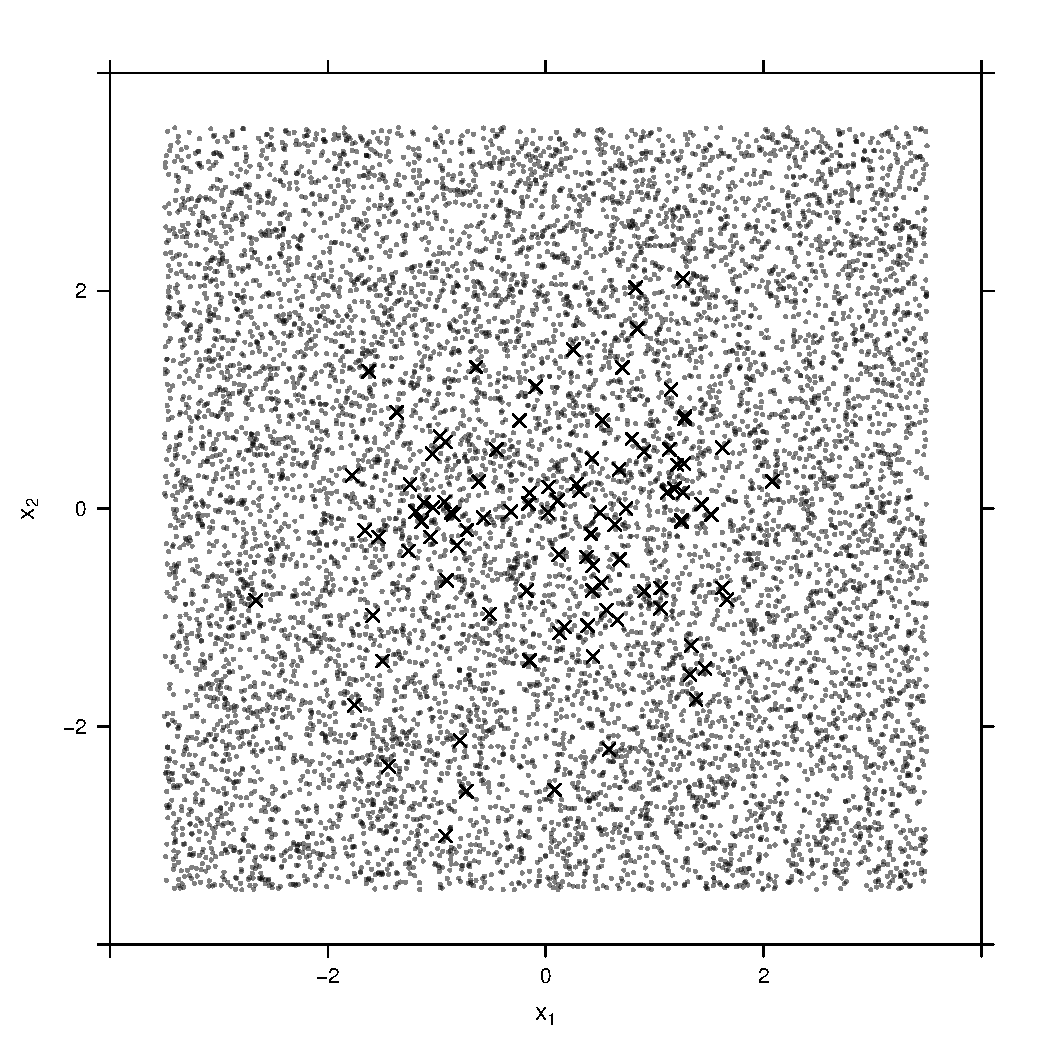
\includegraphics[width=\textwidth]{results/unif_100_1.0_1h/output/population_and_incidents_scatter}
        \caption{100 incidents}
    \end{subfigure}
    \begin{subfigure}{0.45\textwidth}
        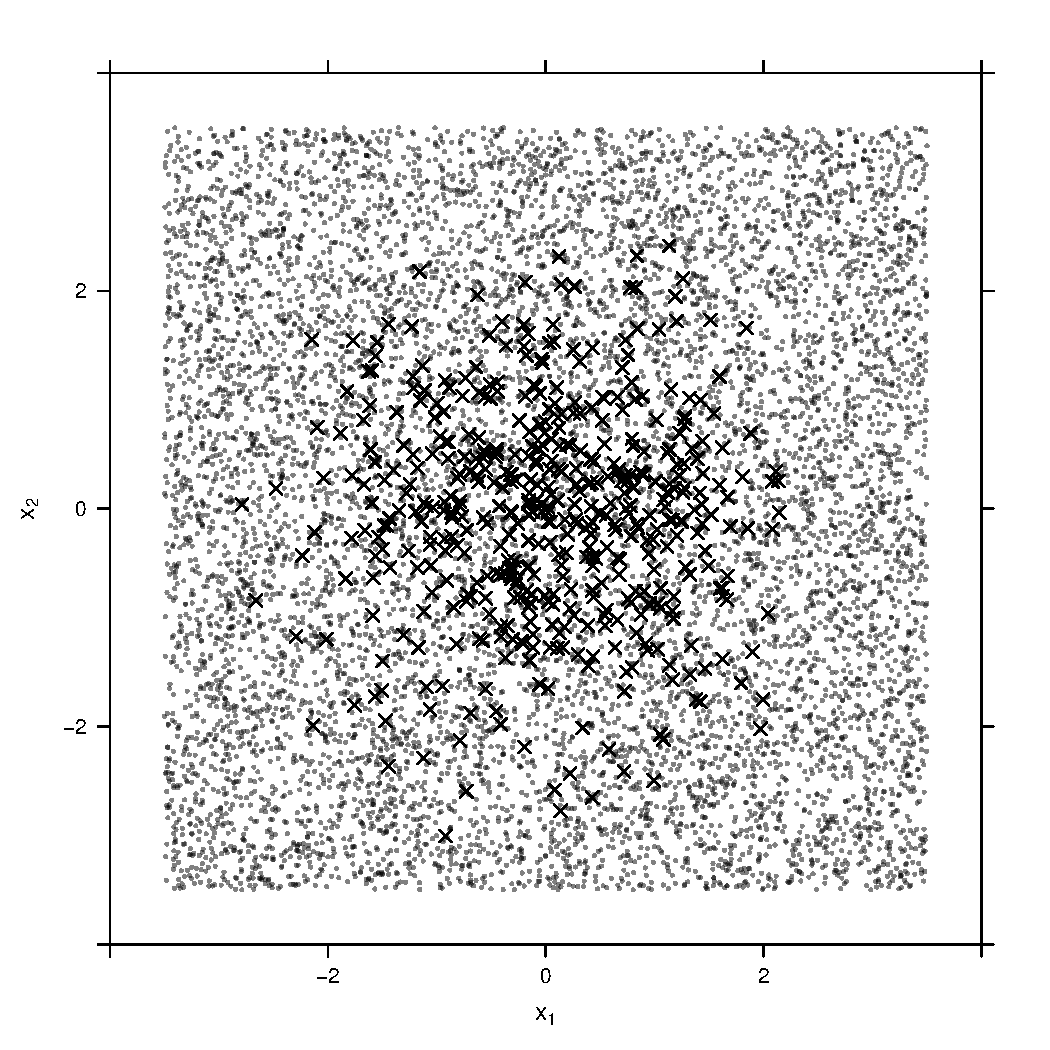
\includegraphics[width=\textwidth]{results/unif_500_1.0_1h/output/population_and_incidents_scatter}
        \caption{500 incidents}
    \end{subfigure}
        \caption{A single realization of different \glspl{factor} from a single-peak risk on a uniform population}
        \label{fig:one_sample:unif_NCases_1h}
\end{figure}

According to the theory developed in \Cref{sec:theory:bandwidth},
the bandwidth should decrease as the \textit{observed} sample size increases according to the formula

\begin{equation}
    \label{eq:h_opt}
    \gls{h_opt} = O(n^{-\frac{1}{6}}) \text{.}
\end{equation}

\Cref{tab:results:bandwidth_vs_mu} compares the selected bandwidths and \gls{nmise} obtained for different \glspl{factor},
since this is the variable which we control.
We observe that all of the bandwidths decrease as \gls{mu} increases.
When there is a power relationship as in \Cref{eq:h_opt} above, we can take the logarithm of both variables to produce a linear relationship.
The slope of the line in the log-log equation is equal to the power of the original equation.
\Cref{fig:results:bandwidth_by_incidents} shows log-log plots of the observed bandwidths that were obtained by the various selection mechanisms.
We have fit a line to each plot to show the linear relationship in the log-log equations, and hence the power relationship between the bandwidths selected by the different mechanisms and the sample size, represented by \gls{factor}.
The observed values for the power of $n$ as represented by $N_I$ are shown in \Cref{tab:results:bandwidth_alpha_by_selector}.

%latex.default(df, file = "h_per_mu.tex", title = "h_per_mu",     where = "htbp", label = "tab:results:bandwidth_vs_mu", rowname = NULL,     booktabs = TRUE, cgroup = c("", "Mean Bandwidths", "NMISE"),     n.cgroup = c(1, 5, 3), colheads = c("$N_I$", "$h_{o1}$",         "$h_{o2}$", "$h_{s}$", "$h_{cv1}$", "$h_{cv2}$", "Oracle",         "Silverman", "CV"), cdec = c(0, rep(1, 5), rep(3, 3)),     caption.loc = "bottom", caption = "Bandwidth and accuracy by expected number of incidents for uniform population of 10,000 with single-peak risk function, spread of 1.0. The NMISE values are scaled by $10^9$.",     caption.lot = "Bandwidth and accuracy by expected number of incidents")%
\begin{table}[htbp]
\begin{center}
\begin{tabular}{rcrrrrrcrrr}
\toprule
\multicolumn{1}{c}{\bfseries }&\multicolumn{1}{c}{\bfseries }&\multicolumn{5}{c}{\bfseries Mean Bandwidths}&\multicolumn{1}{c}{\bfseries }&\multicolumn{3}{c}{\bfseries NMISE}\tabularnewline
\cline{3-7} \cline{9-11}
\multicolumn{1}{c}{$N_I$}&\multicolumn{1}{c}{}&\multicolumn{1}{c}{$h_{o1}$}&\multicolumn{1}{c}{$h_{o2}$}&\multicolumn{1}{c}{$h_{s}$}&\multicolumn{1}{c}{$h_{cv1}$}&\multicolumn{1}{c}{$h_{cv2}$}&\multicolumn{1}{c}{}&\multicolumn{1}{c}{Oracle}&\multicolumn{1}{c}{Silverman}&\multicolumn{1}{c}{CV}\tabularnewline
\midrule
$  50$&&$1.5$&$1.5$&$1.0$&$1.4$&$1.4$&&$3.541$&$5.718$&$5.438$\tabularnewline
$ 100$&&$1.3$&$1.4$&$0.9$&$1.3$&$1.2$&&$2.220$&$3.526$&$3.398$\tabularnewline
$ 200$&&$1.2$&$1.2$&$0.8$&$1.1$&$1.1$&&$1.324$&$2.085$&$1.988$\tabularnewline
$ 500$&&$1.1$&$1.0$&$0.7$&$0.9$&$0.9$&&$0.679$&$1.067$&$0.959$\tabularnewline
$1000$&&$0.9$&$0.9$&$0.6$&$0.9$&$0.8$&&$0.382$&$0.621$&$0.541$\tabularnewline
\bottomrule
\end{tabular}
\caption[Bandwidth and accuracy by expected number of incidents]{Bandwidth and accuracy by expected number of incidents for uniform population of 10,000 with single-peak risk function, spread of 1.0. The NMISE values are scaled by $10^9$.\label{tab:results:bandwidth_vs_mu}}\end{center}
\end{table}


%latex.default(df.alpha, file = "alpha_by_selector.tex", title = "alpha_by_selector",     where = "htbp", label = "tab:results:bandwidth_alpha_by_selector",     rowname = NULL, cdec = c(0, 3), caption.loc = "bottom", caption = "Bandwidth onvergence rate $\\alpha$ of for different bandwidth selectors for a single-peak risk function with spread of 1.0 on a uniform population of 10,000.",     caption.lot = "Bandwidth convergence rate of bandwidth selectors")%
\begin{table}[htbp]
\begin{center}
\begin{tabular}{lr}
\hline\hline
\multicolumn{1}{c}{Selector}&\multicolumn{1}{c}{Slope}\tabularnewline
\hline
Oracle Bandwidth $x_1$&$-0.156$\tabularnewline
Oracle Bandwidth $x_1$&$-0.179$\tabularnewline
Silverman&$-0.167$\tabularnewline
CV Bandwidth $x_1$&$-0.171$\tabularnewline
CV Bandwidth $x_2$&$-0.205$\tabularnewline
Theory&$-0.167$\tabularnewline
\hline
\end{tabular}
\caption[Bandwidth convergence rate of bandwidth selectors]{Bandwidth onvergence rate $\alpha$ of for different bandwidth selectors for a single-peak risk function with spread of 1.0 on a uniform population of 10,000.\label{tab:results:bandwidth_alpha_by_selector}}\end{center}
\end{table}


%%%%%%%%%%%%%%%%%%%%%%%%%%%%%%%%%%%%%%%%%%%%%%%%%
% Selected bandwidth by factor
%%%%%%%%%%%%%%%%%%%%%%%%%%%%%%%%%%%%%%%%%%%%%%%%%
\begin{figure}[htbp]
    \centering
    \begin{subfigure}[t]{0.195\textwidth}
        \centering
        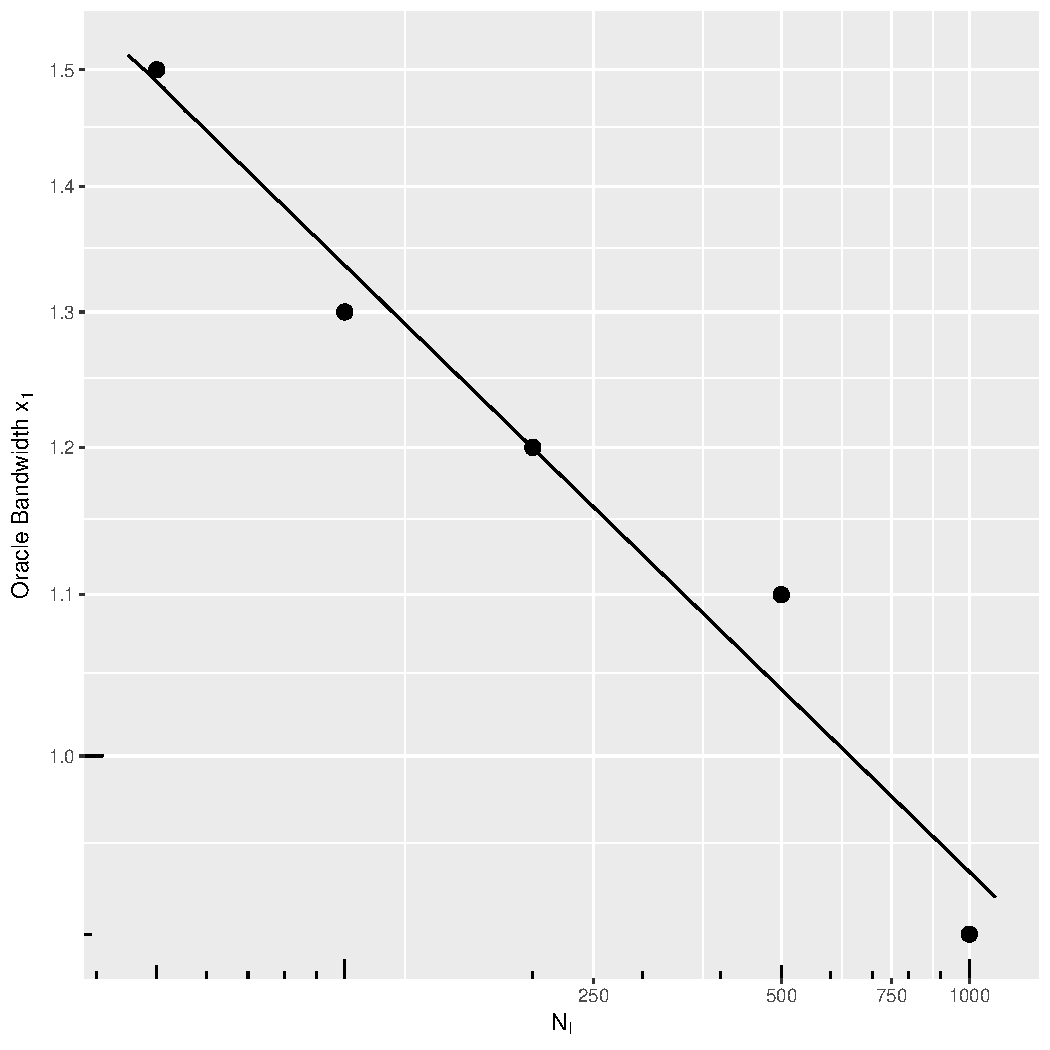
\includegraphics[width=\textwidth]{results/by_h_per_mu/oracle_bandwidth_x1_vs_mu.pdf}
        \subcaption{Oracle bandwidth in $x_1$ direction by \glsentryname{factor}}
    \end{subfigure}
    \begin{subfigure}[t]{0.195\textwidth}
        \centering
        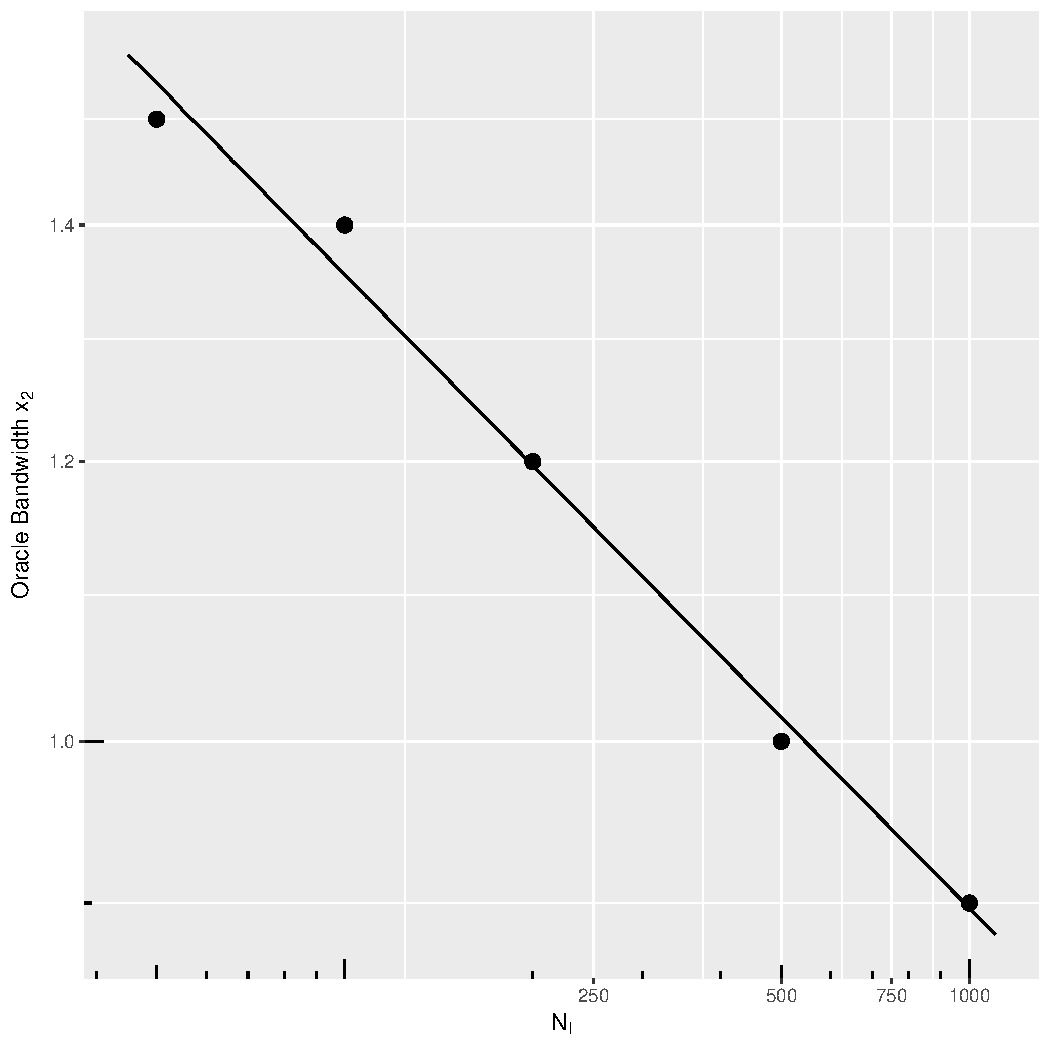
\includegraphics[width=\textwidth]{results/by_h_per_mu/oracle_bandwidth_x2_vs_mu.pdf}
        \subcaption{Oracle bandwidth in $x_2$ direction by \glsentryname{factor}}
    \end{subfigure}
    \begin{subfigure}[t]{0.195\textwidth}
        \centering
        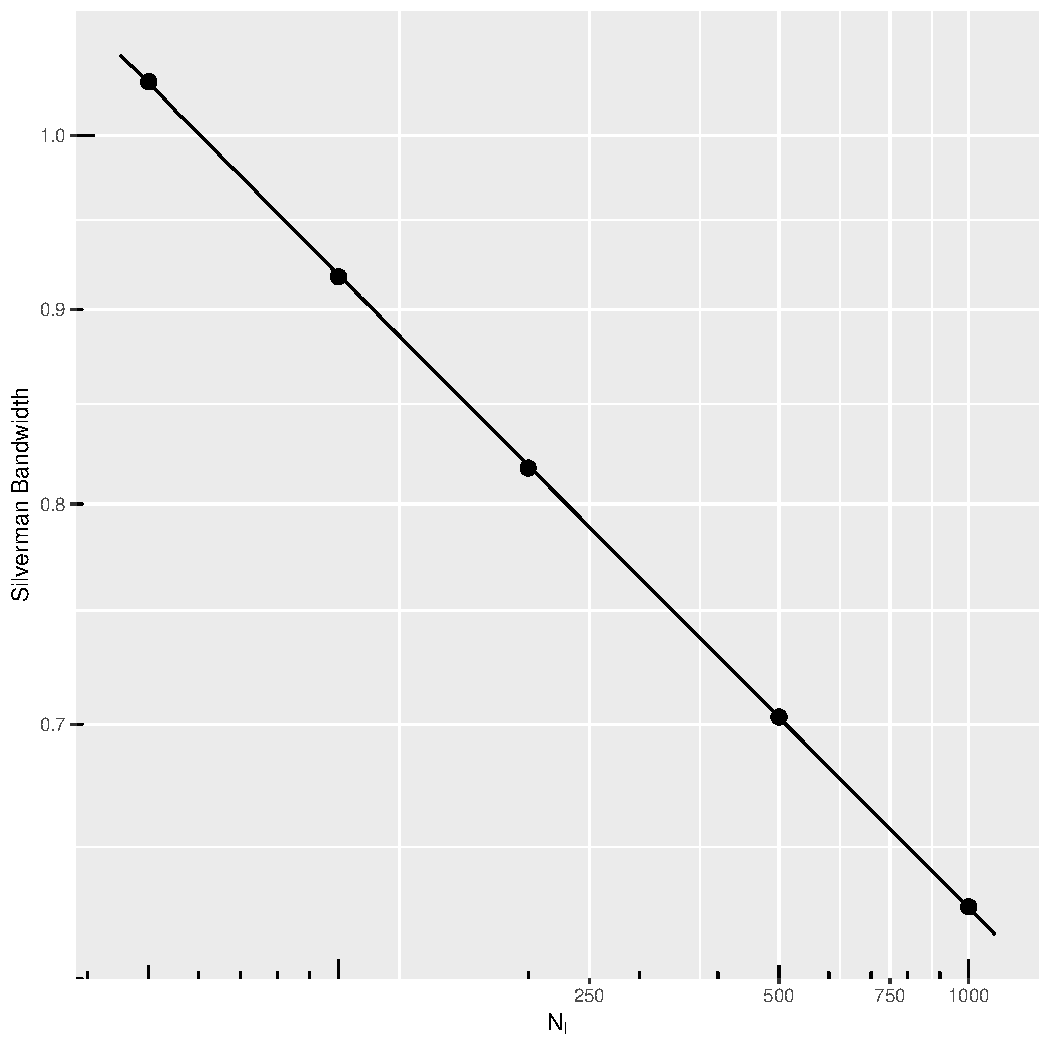
\includegraphics[width=\textwidth]{results/by_h_per_mu/silverman_bandwidth_vs_mu.pdf}
        \subcaption{Mean Silverman bandwidth by \glsentryname{factor}}
    \end{subfigure}
    \begin{subfigure}[t]{0.195\textwidth}
        \centering
        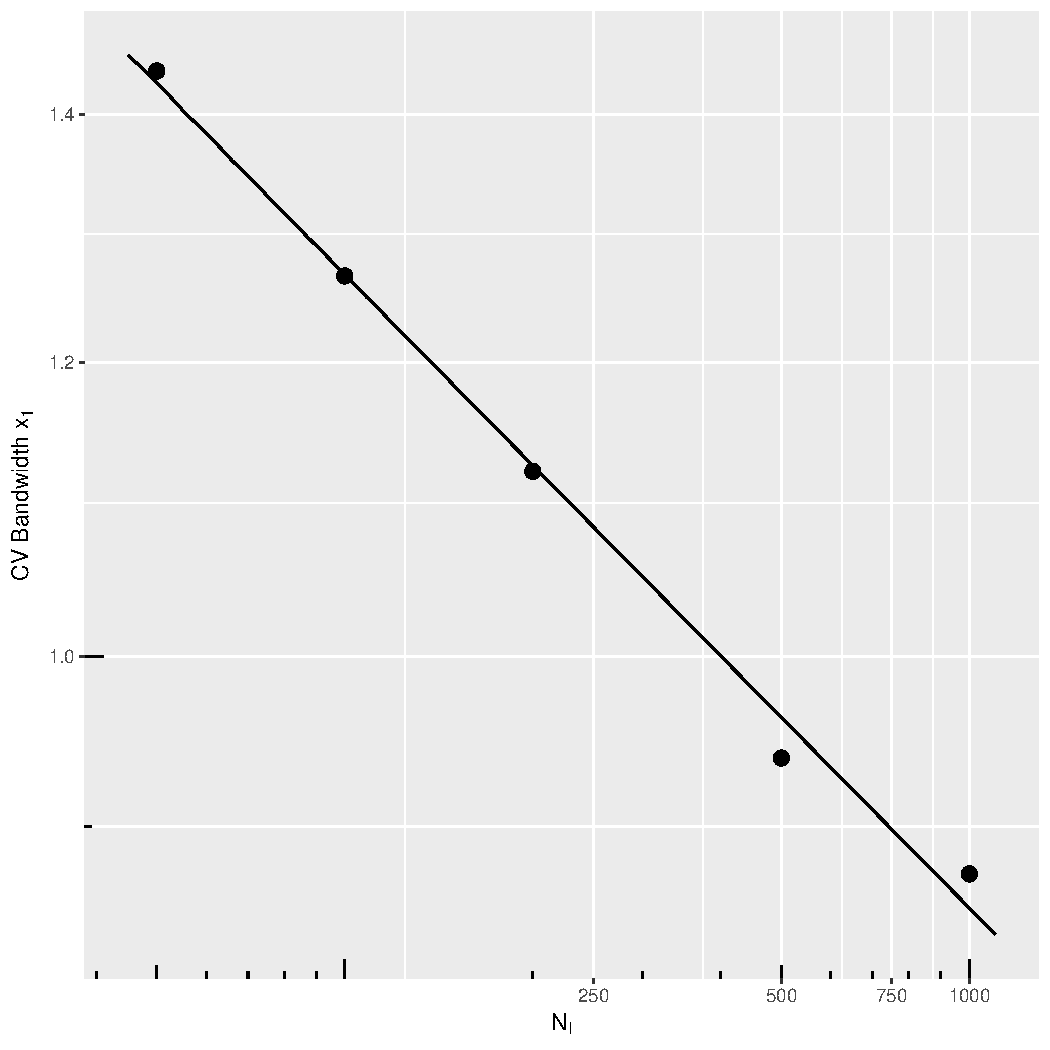
\includegraphics[width=\textwidth]{results/by_h_per_mu/cv_bandwidth_x1_vs_mu.pdf}
        \subcaption{Mean CV bandwidth in $x_1$ direction by \glsentryname{factor}}
    \end{subfigure}
    \begin{subfigure}[t]{0.195\textwidth}
        \centering
        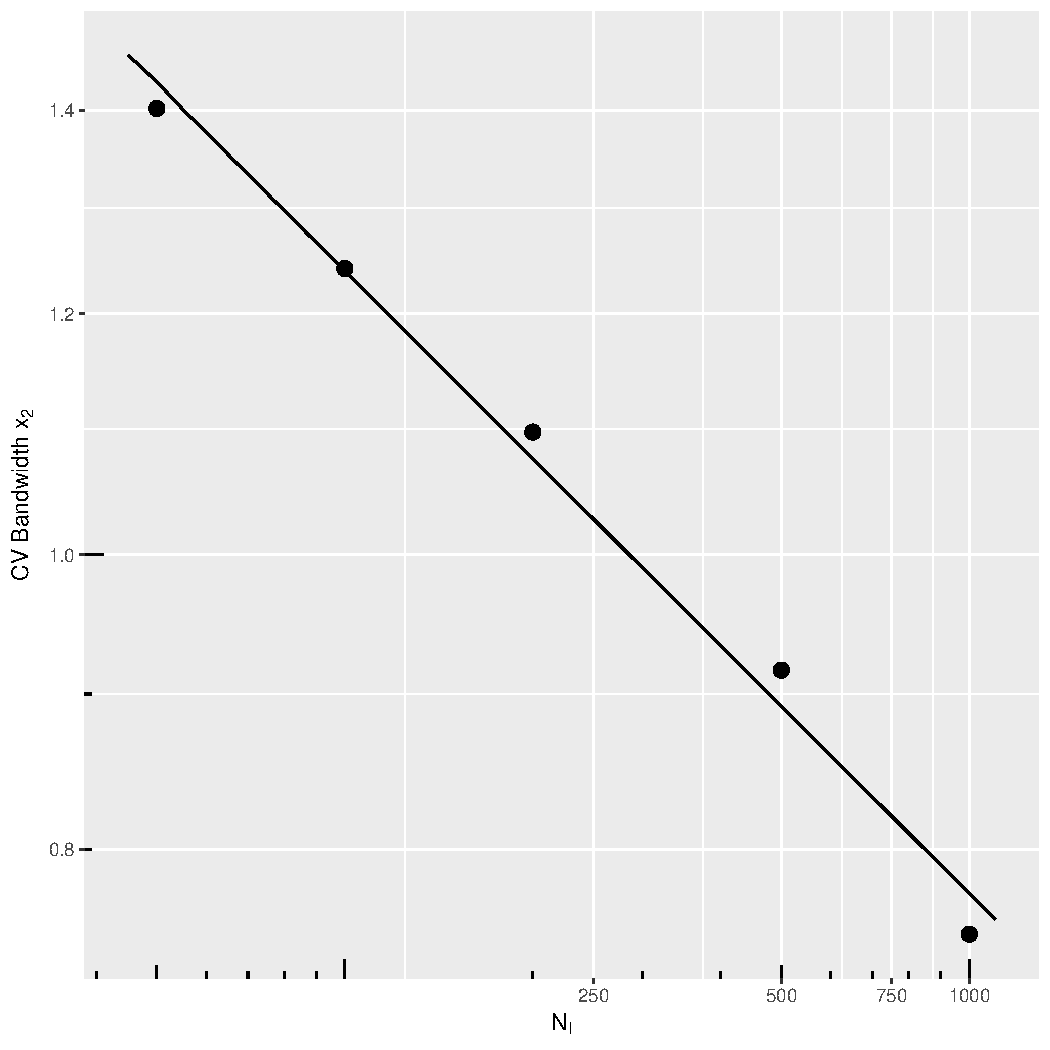
\includegraphics[width=\textwidth]{results/by_h_per_mu/cv_bandwidth_x2_vs_mu.pdf}
        \subcaption{Mean CV bandwidth in $x_2$ direction by \glsentryname{factor}}
    \end{subfigure}
    \caption[Selected bandwidth by \glsentryname{factor}]
        {Log-log plot of selected bandwidth by \glsentryname{factor} for different bandwidth selectors.
        The slope of the log-log plot indicates the power of $n$ in the convergence rate.}
    \label{fig:results:bandwidth_by_incidents}    
\end{figure}

%%%%%%%%%%%%%%%%%%%%%%%%%%%%%%%%%%%%%%%%%%%%%%%%%
% MISE by number of cases
%%%%%%%%%%%%%%%%%%%%%%%%%%%%%%%%%%%%%%%%%%%%%%%%%
\begin{figure}[htbp]
    \centering
    \begin{subfigure}[b]{0.49\textwidth}
        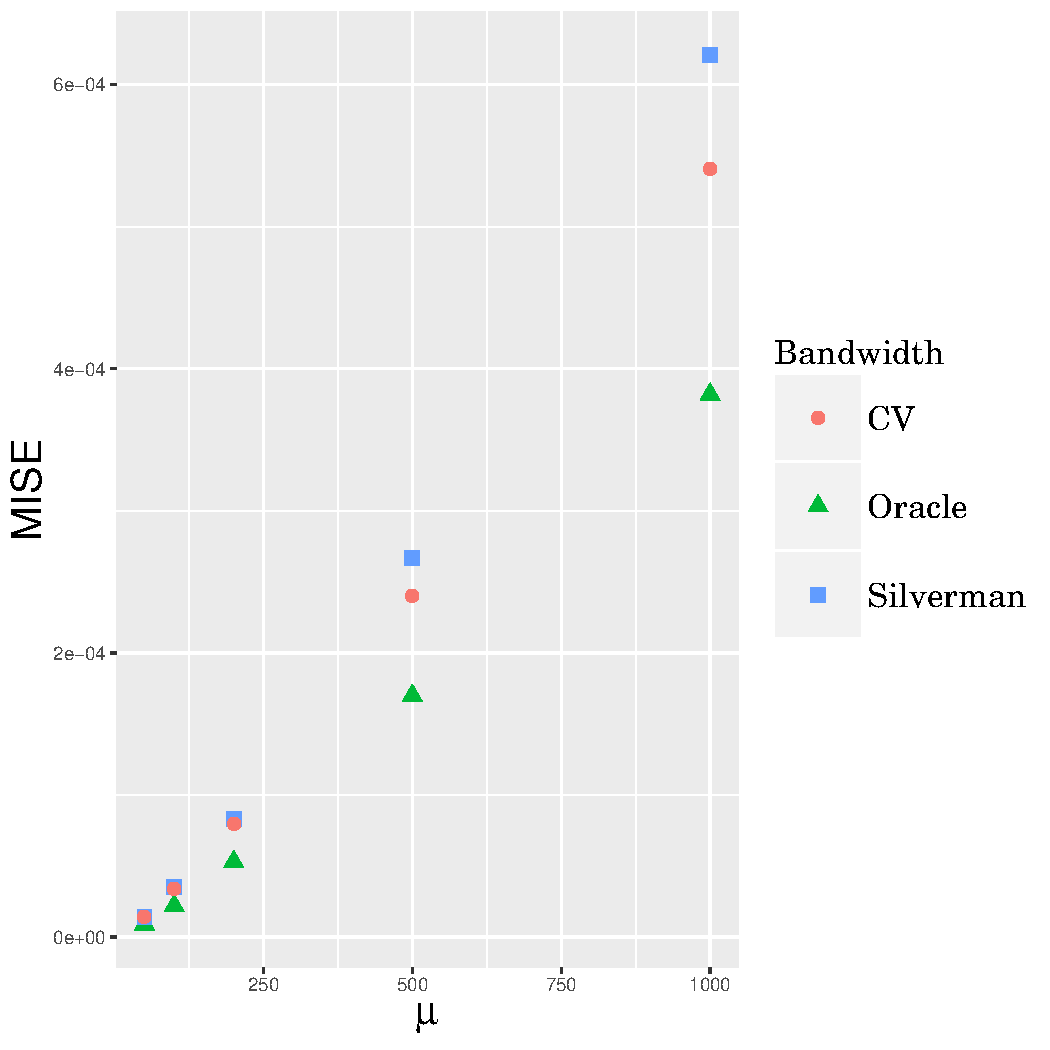
\includegraphics[width=\textwidth]{results/by_num_cases/MISE-vs-cases}
        \subcaption{\glsentryname{mise}}
        \label{fig:ise:unif_NCases_1h:mise}
    \end{subfigure}
    \begin{subfigure}[b]{0.49\textwidth}
        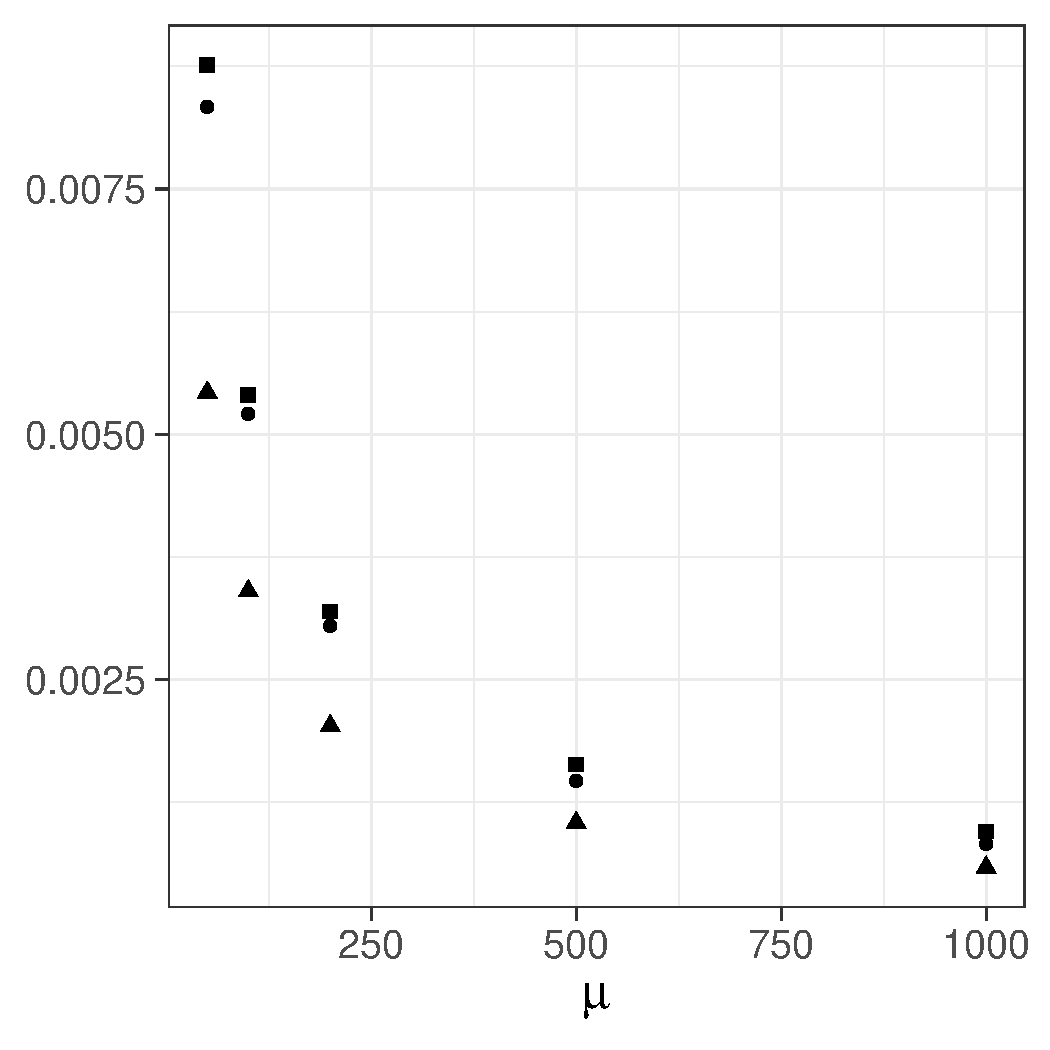
\includegraphics[width=\textwidth]{results/by_num_cases/RMISE-vs-cases}
        \subcaption{\glsentryname{rmise}}
        \label{fig:ise:unif_NCases_1h:rmise}
    \end{subfigure}

    \begin{subfigure}[b]{0.49\textwidth}
        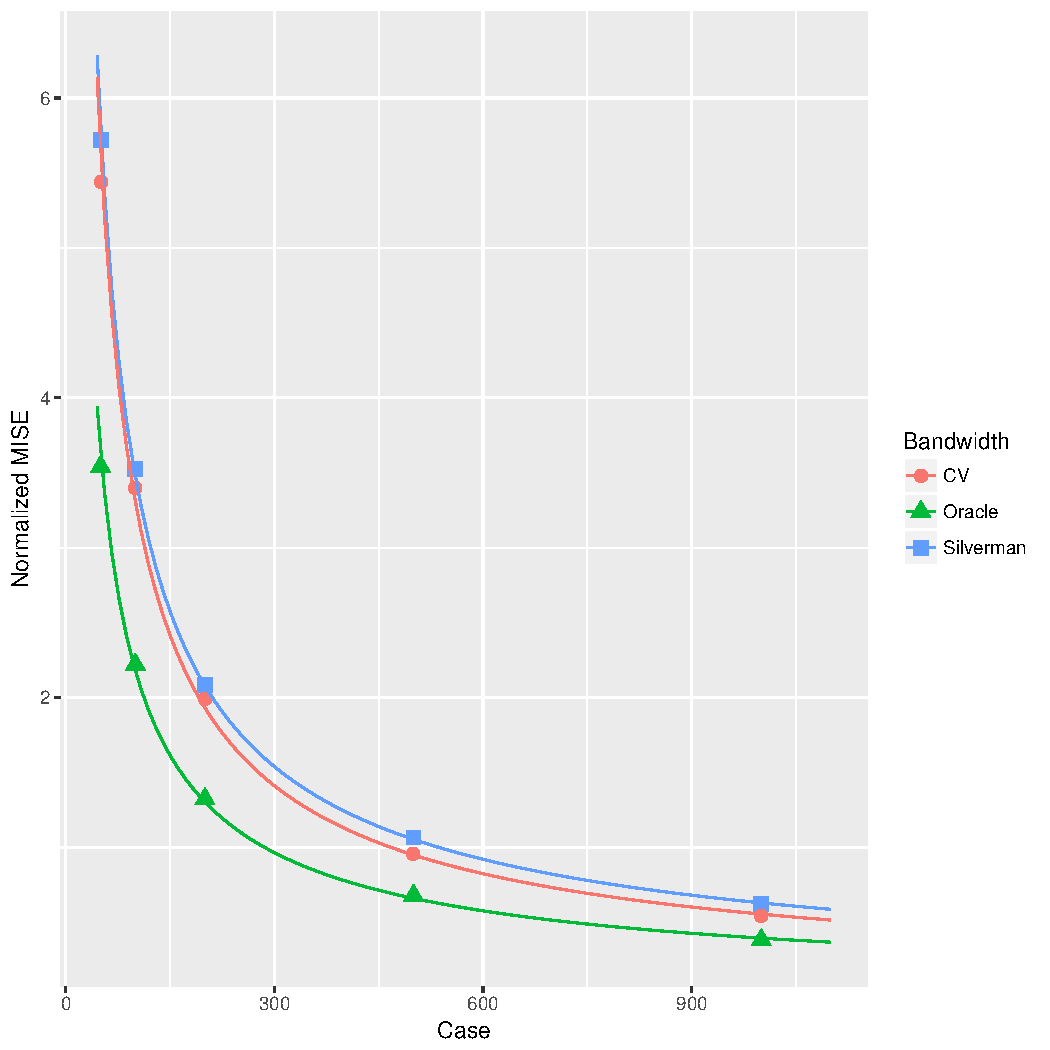
\includegraphics[width=\textwidth]{results/by_num_cases/NMISE-vs-cases}
        \subcaption{\glsentryname{nmise}}
        \label{fig:ise:unif_NCases_1h:nmise}
    \end{subfigure}
    \begin{subfigure}[b]{0.49\textwidth}
        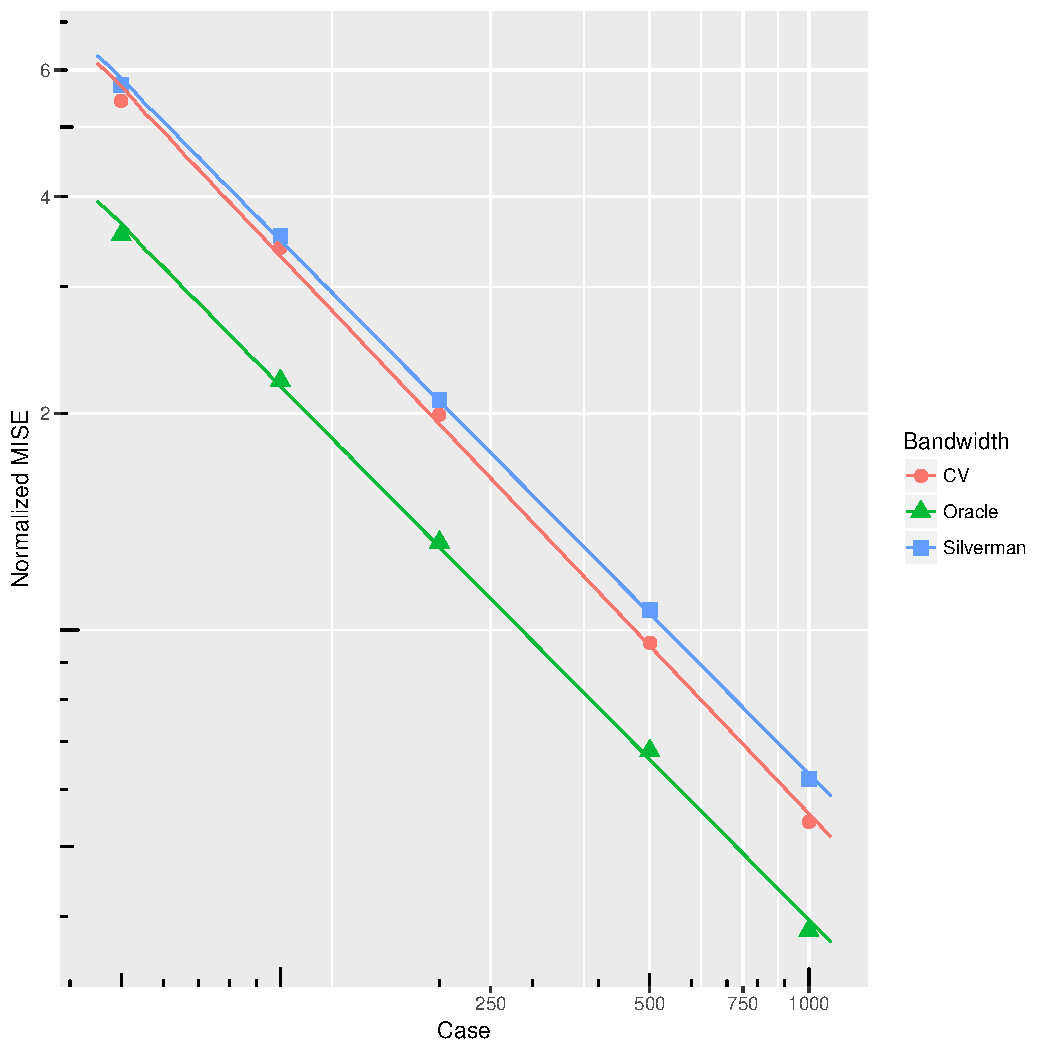
\includegraphics[width=\textwidth]{results/by_num_cases/NMISE-vs-cases-log-log}
        \subcaption{\glsentryname{nmise} log-log}
        \label{fig:ise:unif_NCases_1h:nmise_log_log}
    \end{subfigure}
    \caption{\glsentryname{mise} by number of cases}
    \label{fig:ise:unif_NCases_1h}
\end{figure}

\autoref{fig:ise:unif_NCases_1h} shows the effect of \gls{factor} on the \gls{mise}, \gls{rmise} and on \gls{nmise}:
\autoref{fig:ise:unif_NCases_1h:mise} shows how \gls{mise} increases with \gls{factor}.
One might expect the error to associated with estimating a function to \textit{decrease} as the \gls{factor} increases.
However, the \gls{factor} increases linearly with the intensity function value.
For example, double the number of incidents corresponds to an intensity of twice the value.
This makes comparing the \gls{mise} of estimates of intensity functions difficult,
as the errors will also rise in the same direction.
In order to facilitate the comparison of intensity functions that have different expected number of incidents,
we use the \gls{rmise}and \gls{nmise}.
\Cref{fig:ise:unif_NCases_1h:rmise,fig:ise:unif_NCases_1h:nmise} shows how \gls{rmise} and \gls{nmise} decreases with \gls{factor}.
To test if there is a power relationship between \gls{nmise} and \gls{factor},
we take the logarithms of each variable and fit a line.
\autoref{fig:ise:unif_NCases_1h:nmise_log_log} is a log-log graph,
showing the linear relationship between the logarithm of \gls{nmise} and the logarithm of the \gls{factor}.
This indicates a power relationship between \gls{nmise} and \gls{factor} for each bandwidth selection method is shown in \Cref{tab:results:nmise_convergence_by_num_cases}.
They are all near to $-0.75$.

%latex.default(df.alpha, title = "nmise_convergence_table", where = "htbp",     label = "tab:results:nmise_convergence_by_num_cases", rowname = NULL,     booktabs = TRUE, cdec = c(0, 3), caption.loc = "bottom",     caption = "NMISE onvergence rate by number of cases for different bandwidth selectors for a single-peak risk function with spread of 1.0 on a uniform population of 10,000.",     caption.lot = "NMISE Convergence rate by number of cases for spread 1.0")%
\begin{table}[htbp]
\begin{center}
\begin{tabular}{lr}
\toprule
\multicolumn{1}{c}{Selector}&\multicolumn{1}{c}{Slope}\tabularnewline
\midrule
Oracle&$-0.742$\tabularnewline
Silverman&$-0.741$\tabularnewline
CV&$-0.775$\tabularnewline
\bottomrule
\end{tabular}
\caption[NMISE Convergence rate by number of cases for spread 1.0]{NMISE onvergence rate by number of cases for different bandwidth selectors for a single-peak risk function with spread of 1.0 on a uniform population of 10,000.\label{tab:results:nmise_convergence_by_num_cases}}\end{center}
\end{table}



%%%%%%%%%%%%%%%%%%%%%%%%%%%%%%%%%%%%%%%%%%%%%%%%%%%%%%%%%%%%%%%%%%%%%%%%%%%%%%
%%
%% Section: Effect of risk spread with fixed population
%%
%%%%%%%%%%%%%%%%%%%%%%%%%%%%%%%%%%%%%%%%%%%%%%%%%%%%%%%%%%%%%%%%%%%%%%%%%%%%%%
\section[Effect of risk spread with fixed population]
    {Effect of risk \glsentryname{spread} for a fixed, uniform population of 10,000 and single peak with \glsentryname{spread} 1.0}
\label{sec:results:spread}

%%%%%%%%%%%%%%%%%%%%%%%%%%%%%%%%%%%%%%%%%%%%%%%%%
% Parameter table - spread
%%%%%%%%%%%%%%%%%%%%%%%%%%%%%%%%%%%%%%%%%%%%%%%%%
\begin{table}[htbp]
    \centering
    \begin{tabular}{ll}
        \toprule
        Parameter & Value \\
        \midrule
        Population size & 10,000 \\
        Population \glsentryname{spread} & uniform \\
        Population center & uniform \\
        \Glsentryname{factor} & 100 \\
        Incident \glsentryname{spread} & 0.7, 1.0, 1.4, 2.0, 2.8 \\
        Incident center & (0,0) \\
        \bottomrule
    \end{tabular}
    \caption[Effect of spread with fixed population]
        {Experimental parameter values varying \glsentryname{spread} for a fixed, uniform population of 10,000 and single peak with \glsentryname{spread} 1.0}
    \label{tab:params:results:spread}
\end{table}

In this section we examine and compare the results of five experiments in which we vary the \gls{spread} \gls{sigma_i}
of a single-peak risk function.
The unknown information that one is trying to discover is, how far away from a source of disease risk is safe.
Our question is, under different \glspl{spread}, how accurate is the \gls{dkd}?
Differing \glspl{spread} are analogous to different levels of concentration of the risk of disease is in a specific location.
Another way to look at it is, is how quickly the risk dissipates in space as one moves further away from a single source of disease risk.
We keep the population size constant at 10,000, distributed uniformly throughout the study area.
The risk function for each of the five experiments has a single peak,
centered at the origin,
with a \gls{factor} of 100.
The values of \gls{sigma_i} used in the experiments in this section are 0.7, 1.0, 1.4, 2.0, and 2.8.
The full set of accuracy measures for these cases can be found in \autoref{tab:mean_error_rates:unif_100_0.7_1h}, \autoref{tab:mean_error_rates:unif_100_1.0_1h}, \autoref{tab:mean_error_rates:unif_100_1.4_1h}, \autoref{tab:mean_error_rates:unif_100_2.0_1h}, and \autoref{tab:mean_error_rates:unif_100_2.8_1h} in \autoref{ch:results_tables}.
We note that as in \Cref{sec:results:unif_100_1.0_1h}, the \gls{peak bias} values were positive for the \gls{silverman} bandwidth based estimates.
\autoref{fig:one_sample:unif_Spreads_1h} shows how one realization of incidents, distributed over the population, for \glspl{spread} of 1.0 and 2.8.

%%%%%%%%%%%%%%%%%%%%%%%%%%%%%%%%%%%%%%%%%%%%%%%%%
% Examples showing incident spreads
%%%%%%%%%%%%%%%%%%%%%%%%%%%%%%%%%%%%%%%%%%%%%%%%%
\begin{figure}[htbp]
    \centering
    \begin{subfigure}{0.45\textwidth}
        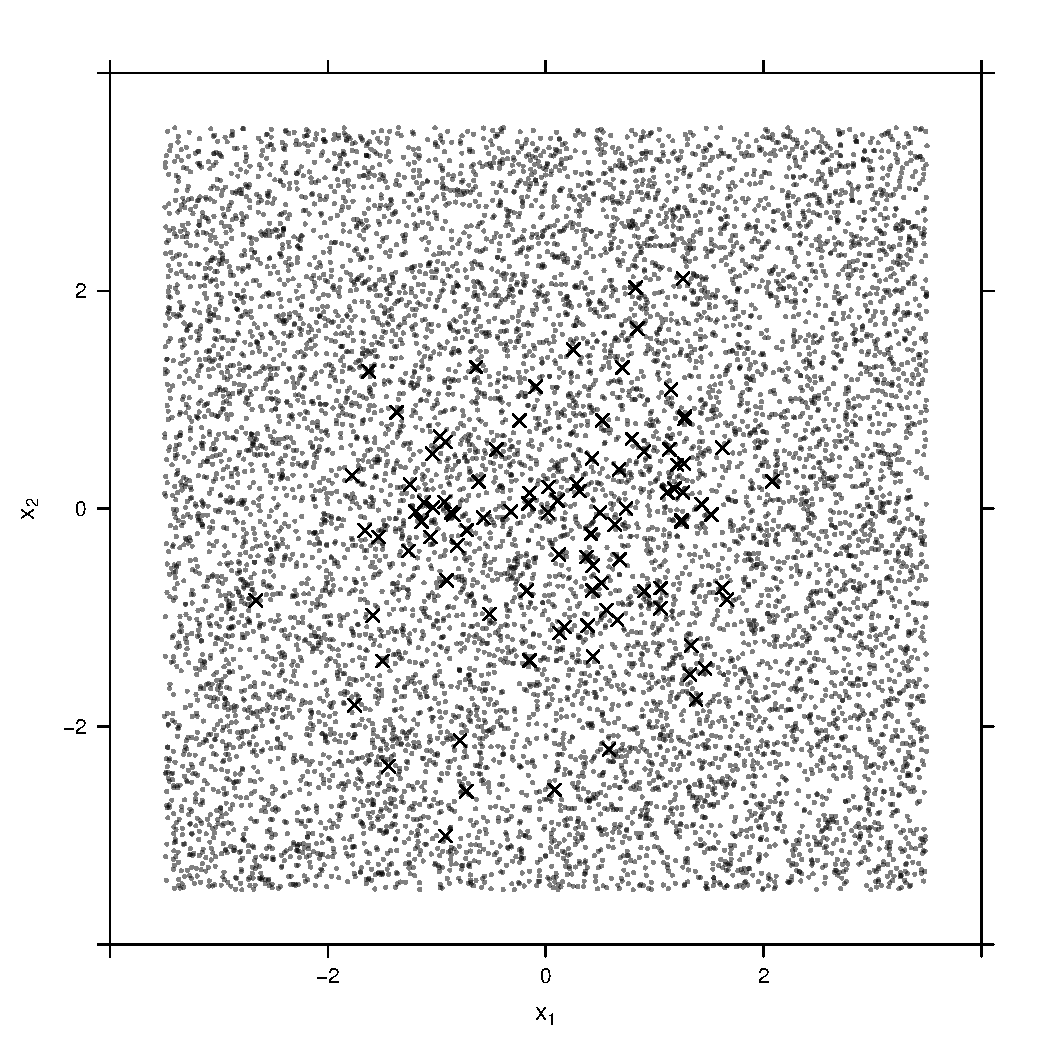
\includegraphics[width=\textwidth]{results/unif_100_1.0_1h/output/population_and_incidents_scatter}
        \caption{\gls{sigma_i} = 1.0}
    \end{subfigure}
    \begin{subfigure}{0.45\textwidth}
        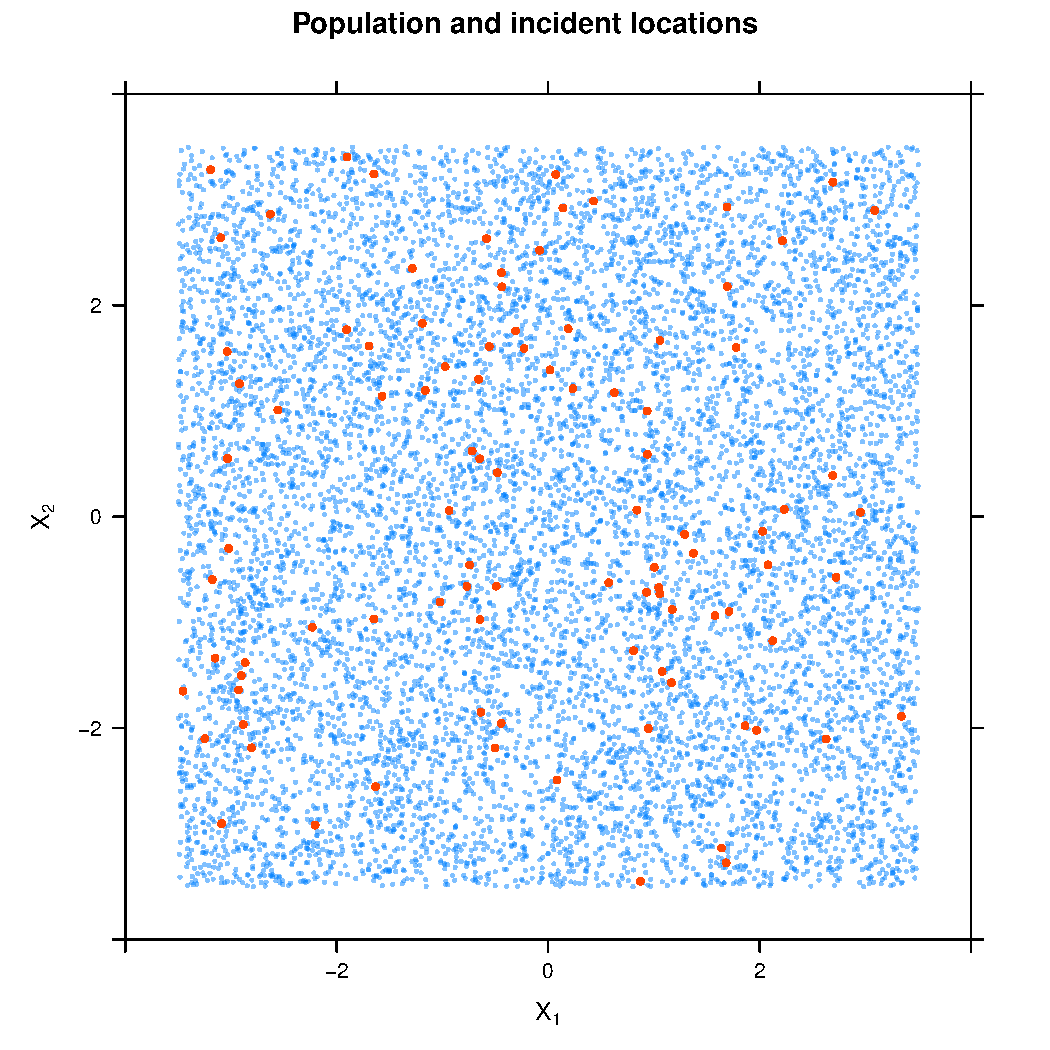
\includegraphics[width=\textwidth]{results/unif_100_2.8_1h/output/population_and_incidents_scatter}
        \caption{\gls{sigma_i} = 2.8}
    \end{subfigure}
    \caption[Examples showing incident spread]
        {A single realization of different incident \glspl{spread} from a single-peak risk on a uniform population}
    \label{fig:one_sample:unif_Spreads_1h}
\end{figure}

The effect of increasing \gls{spread} is that the peak of the risk function becomes less pronounced.
The incidents that are generated by the corresponding \gls{spp} are distributed more evenly and widely throughout the study area \gls{W},
as can be seen in \Cref{fig:one_sample:unif_Spreads_1h}.
We observe the effect of varying \gls{sigma_i} on the selected bandwidths.
The \gls{oracle}, \gls{silverman}, and \gls{cv} bandwidths all increase as the spread increases, as can be seen in \Cref{tab:results:bandwidth_vs_spread}.
This is to be expected, since smaller bandwidths result in decreased smoothing,
which is necessary when the true risk function varies more quickly as is the case with smaller \gls{sigma_i} values.
We note that the \gls{cv} selected bandwidths are closer to \gls{h_opt} as approximated by the \gls{oracle}, than are the \gls{silverman} bandwidths.

%latex.default(df, file = "h_per_spread.tex", title = "h_per_spread",     where = "htbp", label = "tab:results:bandwidth_vs_spread",     rowname = NULL, cgroup = c("", "Mean Bandwidths", "NMISE"),     n.cgroup = c(1, 5, 3), colheads = c("$\\sigma_i$", "$h_{o1}$",         "$h_{o2}$", "$h_{s}$", "$h_{cv1}$", "$h_{cv2}$", "Oracle",         "Silverman", "CV"), cdec = c(1, rep(1, 5), rep(3, 3)),     caption.loc = "bottom", caption = "Bandwidth and accuracy by spread for uniform population of 10,000 with single-peak risk function with expected number of incidents 100. The NMISE values are scaled by $10^9$.",     caption.lot = "Bandwidth and accuracy by spread of incidents")%
\begin{table}[htbp]
\begin{center}
\begin{tabular}{lcrrrrrcrrr}
\hline\hline
\multicolumn{1}{c}{\bfseries }&\multicolumn{1}{c}{\bfseries }&\multicolumn{5}{c}{\bfseries Mean Bandwidths}&\multicolumn{1}{c}{\bfseries }&\multicolumn{3}{c}{\bfseries NMISE}\tabularnewline
\cline{3-7} \cline{9-11}
\multicolumn{1}{c}{$\sigma_i$}&\multicolumn{1}{c}{}&\multicolumn{1}{c}{$h_{o1}$}&\multicolumn{1}{c}{$h_{o2}$}&\multicolumn{1}{c}{$h_{s}$}&\multicolumn{1}{c}{$h_{cv1}$}&\multicolumn{1}{c}{$h_{cv2}$}&\multicolumn{1}{c}{}&\multicolumn{1}{c}{Oracle}&\multicolumn{1}{c}{Silverman}&\multicolumn{1}{c}{CV}\tabularnewline
\hline
0.7&&$0.9$&$1.0$&$0.6$&$0.9$&$0.9$&&$4.151$&$6.976$&$6.667$\tabularnewline
1.0&&$1.3$&$1.4$&$0.9$&$1.3$&$1.2$&&$2.220$&$3.526$&$3.398$\tabularnewline
1.4&&$1.9$&$1.8$&$1.3$&$1.7$&$1.7$&&$1.163$&$1.869$&$1.637$\tabularnewline
2.0&&$2.5$&$2.6$&$1.6$&$2.1$&$2.1$&&$0.642$&$1.187$&$0.919$\tabularnewline
\hline
\end{tabular}
\caption[Bandwidth and accuracy by spread of incidents]{Bandwidth and accuracy by spread for uniform population of 10,000 with single-peak risk function with expected number of incidents 100. The NMISE values are scaled by $10^9$.\label{tab:results:bandwidth_vs_spread}}\end{center}
\end{table}


We also observe that the \gls{nmise} decreases significantly with increasing \gls{sigma_i}.
This provides evidence that the \gls{dkd} may be better suited to situations where the true underlying risk is smoother.
In \Cref{fig:ise:unif_Spreads_1h} we take a closer look at the distributions of \gls{mise}, \gls{rmise}, and \gls{nmise}.
\textbf{We see is that as $\boldsymbol{\gls{sigma_i}}$ increases, both absolute and normalized \gls{mise} decrease but relative \gls{mise} increases.}
This is the same for all bandwidth selection methods.
Since we keep \gls{mu} constant throughout the experiment, we would expect absolute and normalized \gls{mise} behave similarly.
The \gls{rmise} takes a local view of relative error, and here we see that as the \gls{spread} increase, the \gls{mise} decreases but at a slower rate than the true function.


%%%%%%%%%%%%%%%%%%%%%%%%%%%%%%%%%%%%%%%%%%%%%%%%%
% MISE by spread
%%%%%%%%%%%%%%%%%%%%%%%%%%%%%%%%%%%%%%%%%%%%%%%%%
\begin{figure}[htbp]
    \centering
    \begin{subfigure}[t]{0.49\textwidth}
        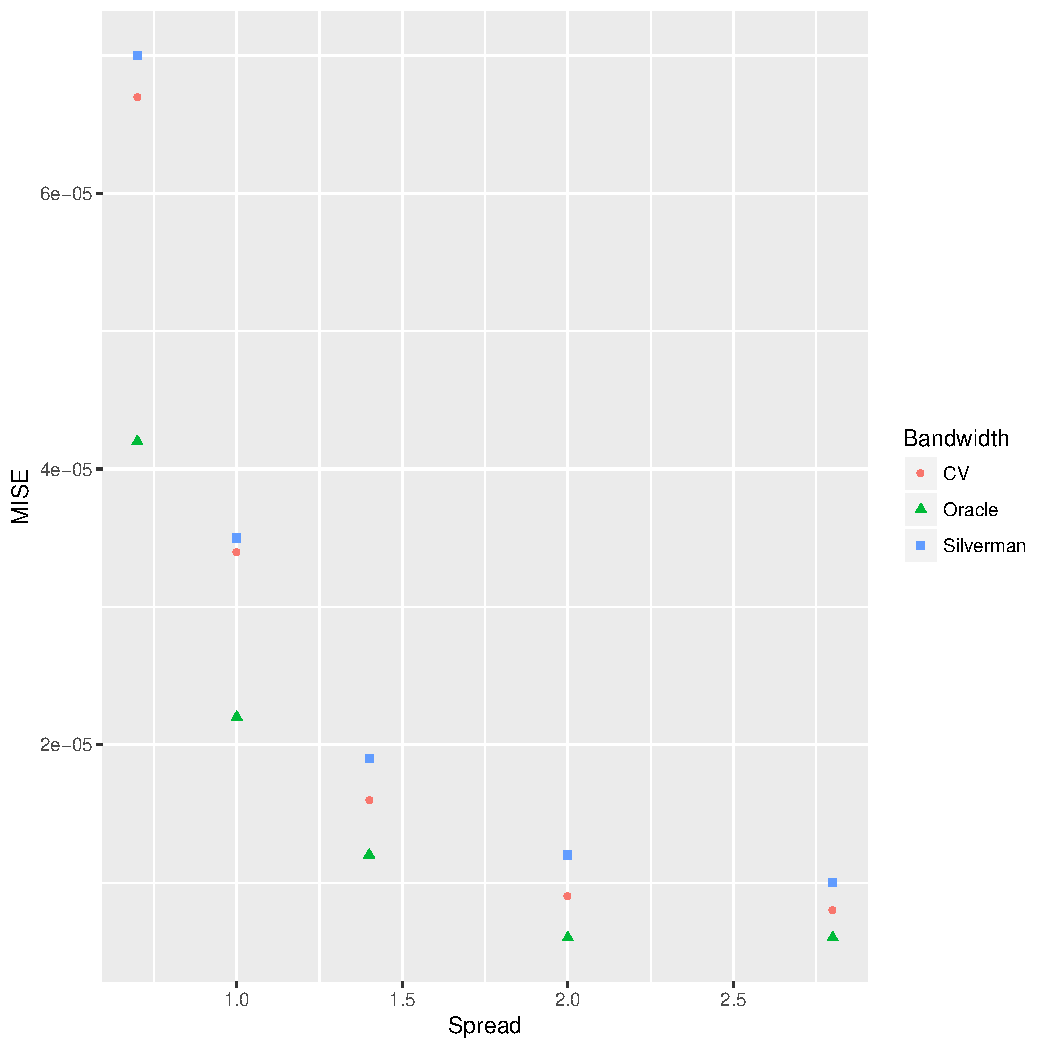
\includegraphics[width=\textwidth]{results/by_cases_spread/MISE-vs-risk-spread}
        \caption{\glsentryname{mise}}
        \label{fig:ise:unif_Spreads_1h:mise}
    \end{subfigure}
    \begin{subfigure}[t]{0.49\textwidth}
        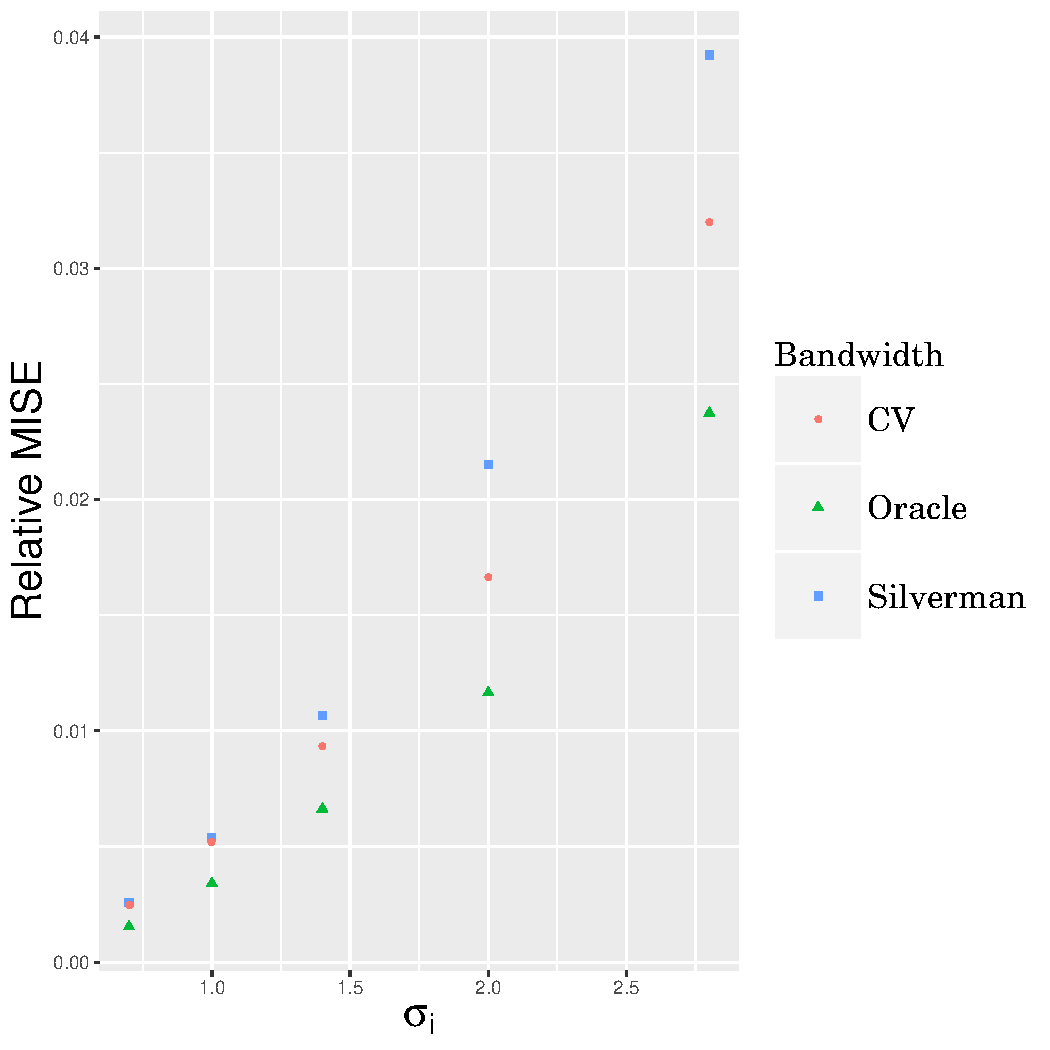
\includegraphics[width=\textwidth]{results/by_cases_spread/RMISE-vs-risk-spread}
        \caption{\glsentryname{rmise}}
        \label{fig:ise:unif_Spreads_1h:rmise}
    \end{subfigure}

    \begin{subfigure}[t]{0.49\textwidth}
        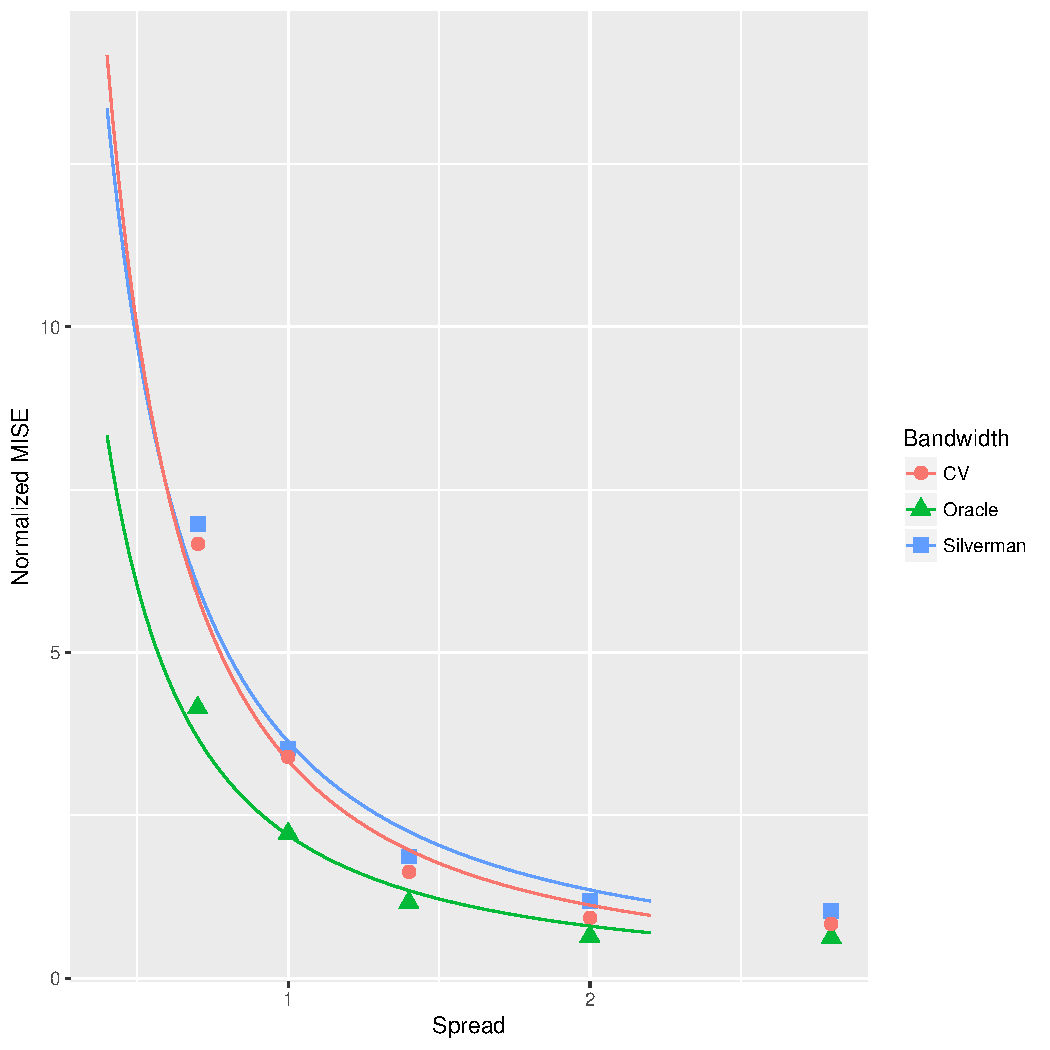
\includegraphics[width=\textwidth]{results/by_cases_spread/NMISE-vs-risk-spread}
        \caption{\glsentryname{nmise}}
        \label{fig:ise:unif_Spreads_1h:nmise}
    \end{subfigure}
    \begin{subfigure}[t]{0.49\textwidth}
        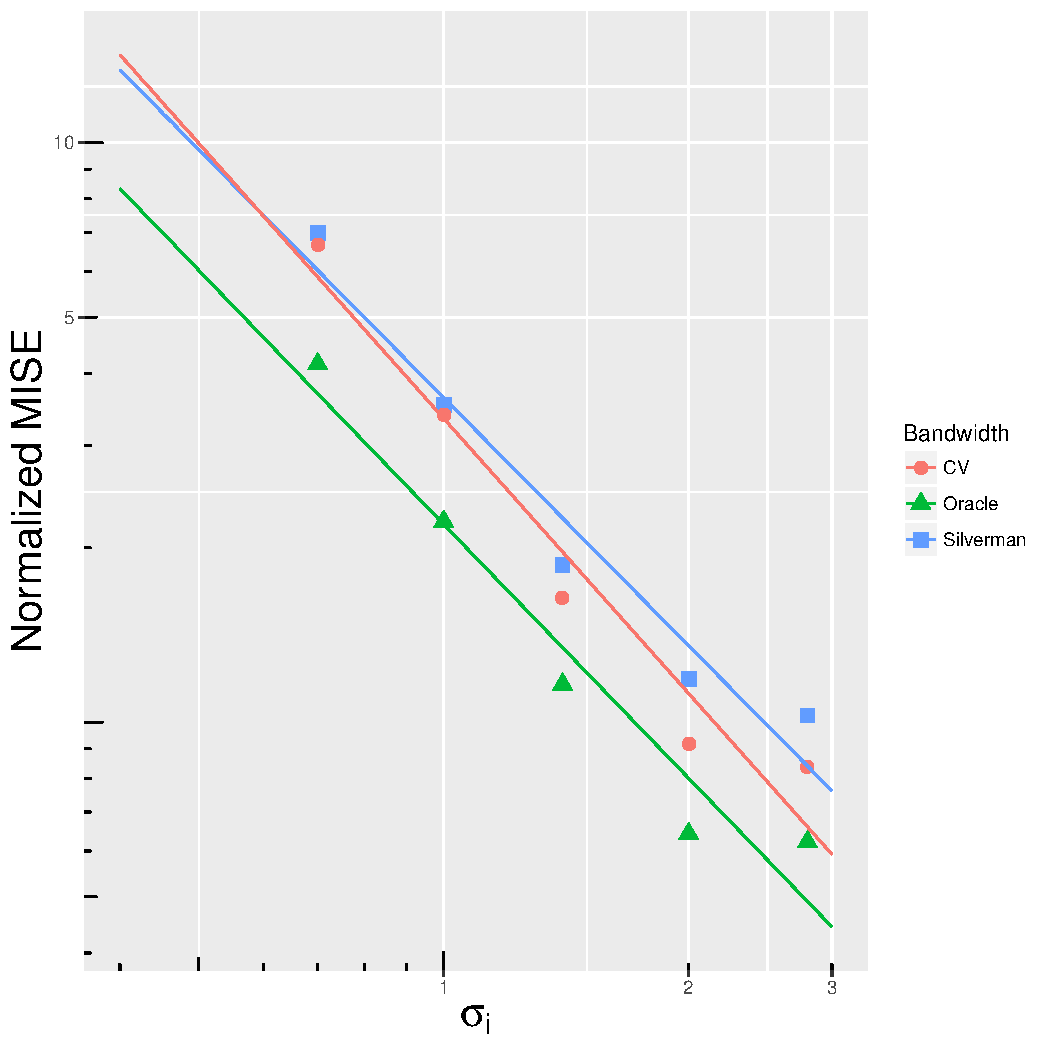
\includegraphics[width=\textwidth]{results/by_cases_spread/NMISE-vs-risk-spread-log-log}
        \caption{\glsentryname{nmise} log-log}
        \label{fig:ise:unif_Spreads_1h:nmise_log_log}
    \end{subfigure}
    \caption[\glsentryname{mise}: by risk \glsentryname{spread}]
        {The effect of \glsentryname{spread} on \glsentryname{mise} for different bandwidth selectors for a single-peak risk function with \gls{factor} 100 on a uniform population of 10,000}
    \label{fig:ise:unif_Spreads_1h}
\end{figure}

We look now at the asymptotic behavior of \gls{nmise} as $\gls{sigma_i} \to \infty$.
From \Cref{fig:ise:unif_Spreads_1h:nmise_log_log} we see a polynomial relationship between \gls{nmise} and \gls{sigma_i} (\Cref{eq:nmise:spread}).
\Cref{tab:results:nmise_convergence_by_cases_spread} shows the slope $\alpha_S$ that we observed for each bandwidth selection method.

\begin{equation}
    \label{eq:nmise:spread}
    \gls{nmise} = O(n^{\alpha_S})
\end{equation}
%latex.default(df.alpha, title = "nmise_convergence_table", where = "htbp",     label = "tab:results:nmise_convergence_by_cases_spread",     rowname = NULL, booktabs = TRUE, cdec = c(0, 3), caption.loc = "bottom",     caption = "NMISE convergence rate by spread for different bandwidth selectors for a single-peak risk function with expected number of incidents 100 on a uniform population of 10,000.",     caption.lot = "NMISE Convergence rate by spread for 100 cases")%
\begin{table}[htbp]
\begin{center}
\begin{tabular}{lr}
\toprule
\multicolumn{1}{c}{Selector}&\multicolumn{1}{c}{Slope}\tabularnewline
\midrule
Oracle&$-1.455$\tabularnewline
Silverman&$-1.421$\tabularnewline
CV&$-1.576$\tabularnewline
\bottomrule
\end{tabular}
\caption[NMISE Convergence rate by spread for 100 cases]{NMISE convergence rate by spread for different bandwidth selectors for a single-peak risk function with expected number of incidents 100 on a uniform population of 10,000.\label{tab:results:nmise_convergence_by_cases_spread}}\end{center}
\end{table}


We now look at the convergence rate of \gls{rmise} as the number of incidents grow.
We see from \Cref{tab:results:rmise_convergence_by_cases_and_spread} that independent of bandwidth selection method,
there is no clear pattern in the convergence rates.
For each value of the \gls{spread}, there is negative polynomial convergence as incidents go to infinity.
However, we did not observe a monotonic growth rate of the exponent with the spread.

%latex.default(df, title = "rmise_convergence_table", where = "htbp",     label = "tab:results:rmise_convergence_by_cases_and_spread",     rowname = NULL, booktabs = TRUE, cdec = c(1, rep(3, 3)),     caption.loc = "bottom", caption = "RMISE convergence rates by case for different bandwidth selectors and different spreads when the population of 10,000 is uniformly distributed.",     caption.lot = "RMISE Convergence rate by case for different spreads")%
\begin{table}[htbp]
\begin{center}
\begin{tabular}{rrrr}
\toprule
\multicolumn{1}{c}{decay}&\multicolumn{1}{c}{alphaO}&\multicolumn{1}{c}{alphaS}&\multicolumn{1}{c}{alphaC}\tabularnewline
\midrule
$0.7$&$-0.301$&$-0.431$&$-0.418$\tabularnewline
$1.0$&$-0.742$&$-0.741$&$-0.775$\tabularnewline
$1.4$&$-0.666$&$-0.701$&$-0.712$\tabularnewline
$2.0$&$-0.604$&$-0.652$&$-0.670$\tabularnewline
$Inf$&$-0.327$&$-0.377$&$-0.354$\tabularnewline
\bottomrule
\end{tabular}
\caption[RMISE Convergence rate by case for different spreads]{RMISE convergence rates by case for different bandwidth selectors and different spreads when the population of 10,000 is uniformly distributed.\label{tab:results:rmise_convergence_by_cases_and_spread}}\end{center}
\end{table}



%%%%%%%%%%%%%%%%%%%%%%%%%%%%%%%%%%%%%%%%%%%%%%%%%%%%%%%%%%%%%%%%%%%%%%%%%%%%%%
%%
%% Section: Varying the sample size for fixed intensity
%%
%%%%%%%%%%%%%%%%%%%%%%%%%%%%%%%%%%%%%%%%%%%%%%%%%%%%%%%%%%%%%%%%%%%%%%%%%%%%%%
\section{Varying the population and sample size for fixed intensity}
\label{sec:results:unifNpop_1h}

%%%%%%%%%%%%%%%%%%%%%%%%%%%%%
% Parameter table
%%%%%%%%%%%%%%%%%%%%%%%%%%%%%
\begin{table}[htbp]
    \centering
    \begin{tabular}{ll}
        \toprule
        Parameter & Value \\
        \midrule
        Population size & 5,000, 10,000, 20,000, 50,000, 100,000 \\
        Population \gls{spread} & uniform \\
        Population center & uniform \\
        \Gls{factor} & 50, 100, 200, 500, 1000 \\
        Incident \gls{spread} & 1.0 \\
        Incident center & (0,0) \\
        \bottomrule
    \end{tabular}
    \caption{Parameters used for varying the sample size for fixed intensity}
    \label{tab:params:unifNpop_1h}
\end{table}

We next examine the effect of increasing the sample size, while keeping the risk intensity function fixed.
Unlike what we did in \Cref{sec:results:number_of_incidents} where we fixed the size of the population and allowed the risk function to change,
here we fix the risk function and change the population size.
This is analogous to increasing the size of the population under study, for example by increasing the study area.
In order to do this, we increase the population size and the \gls{factor} proportionately.
For example, in one experiment \gls{factor} is 50 and the population is 5,000,
and in the next experiment the \gls{factor} is 100 and the population is 10,000.
For this set of experiments, the population is uniformly distributed and the risk intensity has a single peak in the center with a fixed \gls{sigma_i} of 1.0.
Mean and standard deviations of accuracy measures for the experiments of this section are found in \Cref{tab:mean_error_rates:unif5k_50_1.0_1h,tab:mean_error_rates:unif10k_100_1.0_1h,tab:mean_error_rates:unif20k_200_1.0_1h,tab:mean_error_rates:unif50k_500_1.0_1h,tab:mean_error_rates:unif100k_1000_1.0_1h}.

\Cref{fig:one_sample:unifNpop_1h} shows two populations of size 10,000 and 50,000,
as represented by the small points,
and two corresponding realizations of \glspl{incident},
with sizes 100 and 500 respectively,
indicated by triangles.
In both cases,
the population is distributed uniformly throughout the study area,
while the incident samples are concentrated around the peak in the center.

%%%%%%%%%%%%%%%%%%%%%%%%%%%%%%%%%%%%%%%%%%%%%%%%%
% Examples showing sample size
%%%%%%%%%%%%%%%%%%%%%%%%%%%%%%%%%%%%%%%%%%%%%%%%%
\begin{figure}[htbp]
    \centering
    \begin{subfigure}{0.45\textwidth}
        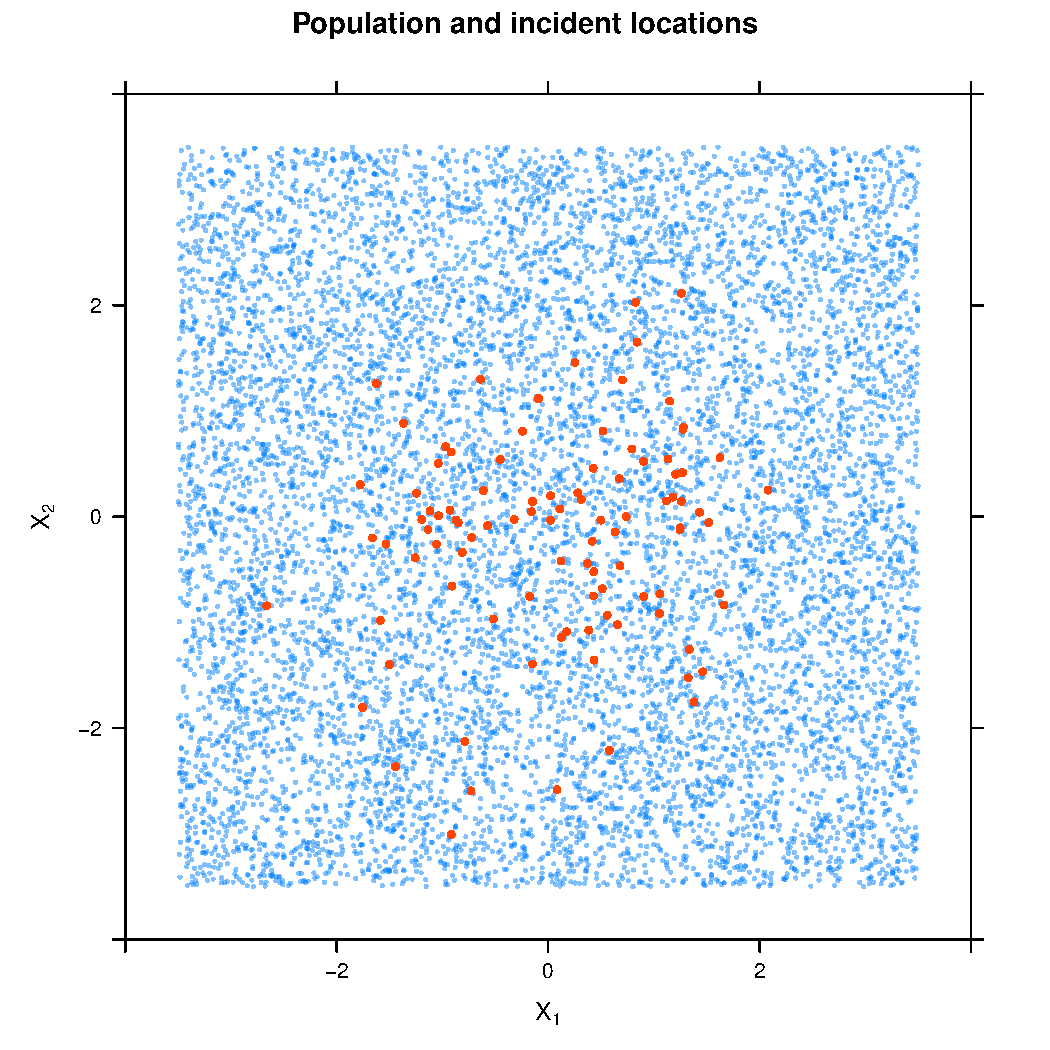
\includegraphics[width=\textwidth]{results/unif10k_100_1.0_1h/output/population_and_incidents_scatter}
        \caption{100 incidents from population of 10,000}
    \end{subfigure}
    \begin{subfigure}{0.45\textwidth}
        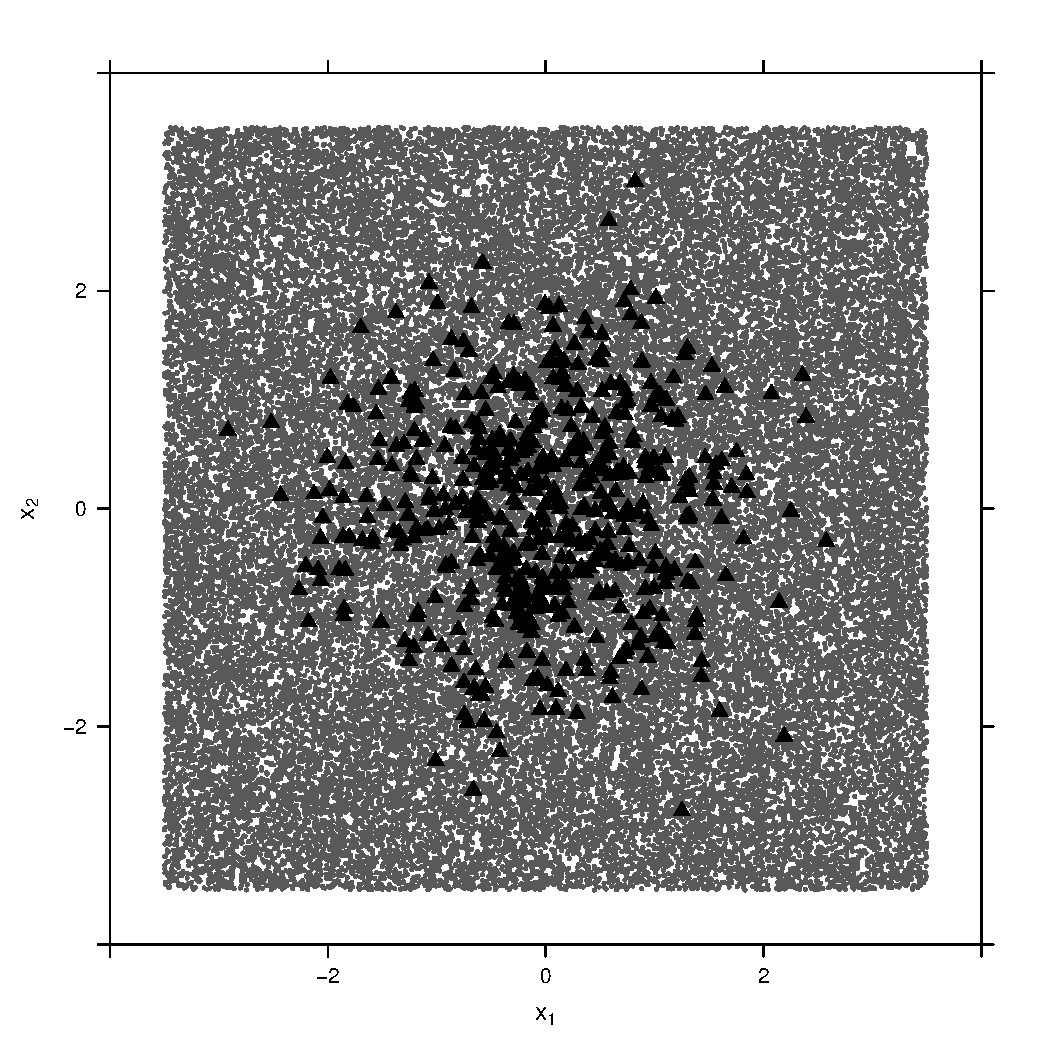
\includegraphics[width=\textwidth]{results/unif50k_500_1.0_1h/output/population_and_incidents_scatter}
        \caption{500 incidents from population of 50,000}
    \end{subfigure}
    \caption[Examples showing sample size]
        {A single realization of different sample sizes from a single-peak risk on a uniform population, obtained by varying the \gls{factor} and population size in lockstep while keeping the risk function $\lambda \xvec$ fixed}
    \label{fig:one_sample:unifNpop_1h}
\end{figure}

%%%%%%%%%%%%%%%%%%%%%%%%%%%%%%%%%%%%%%%%%%%%%%%%%
% MISE by sample + population
%%%%%%%%%%%%%%%%%%%%%%%%%%%%%%%%%%%%%%%%%%%%%%%%%
\begin{figure}[htbp]
    \centering
    \begin{subfigure}[b]{0.49\textwidth}
        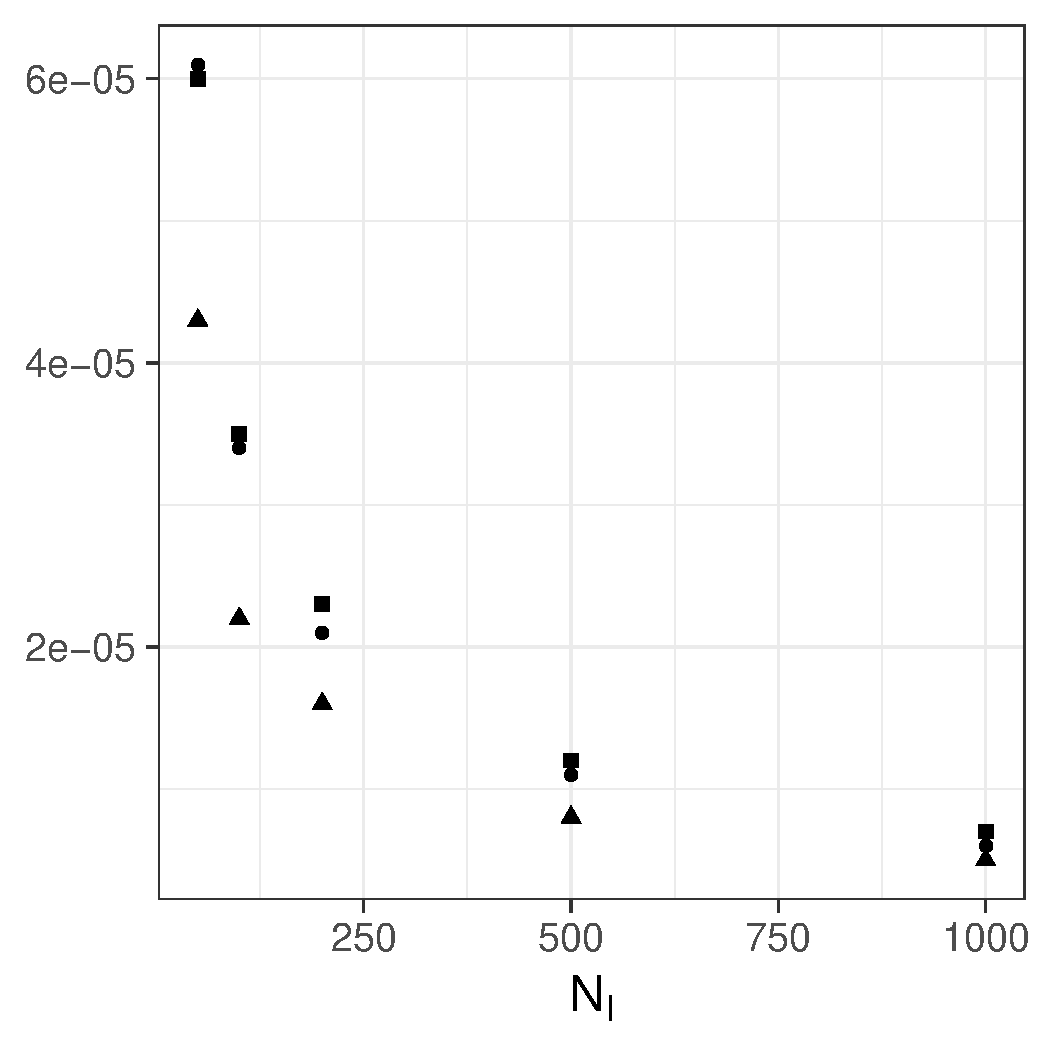
\includegraphics[width=\textwidth]{results/by_pop_size/MISE-vs-population}
        \caption{\glsentryname{mise}}
        \label{fig:ise:unifNpop_1h:mise}
    \end{subfigure}
    \begin{subfigure}[b]{0.49\textwidth}
        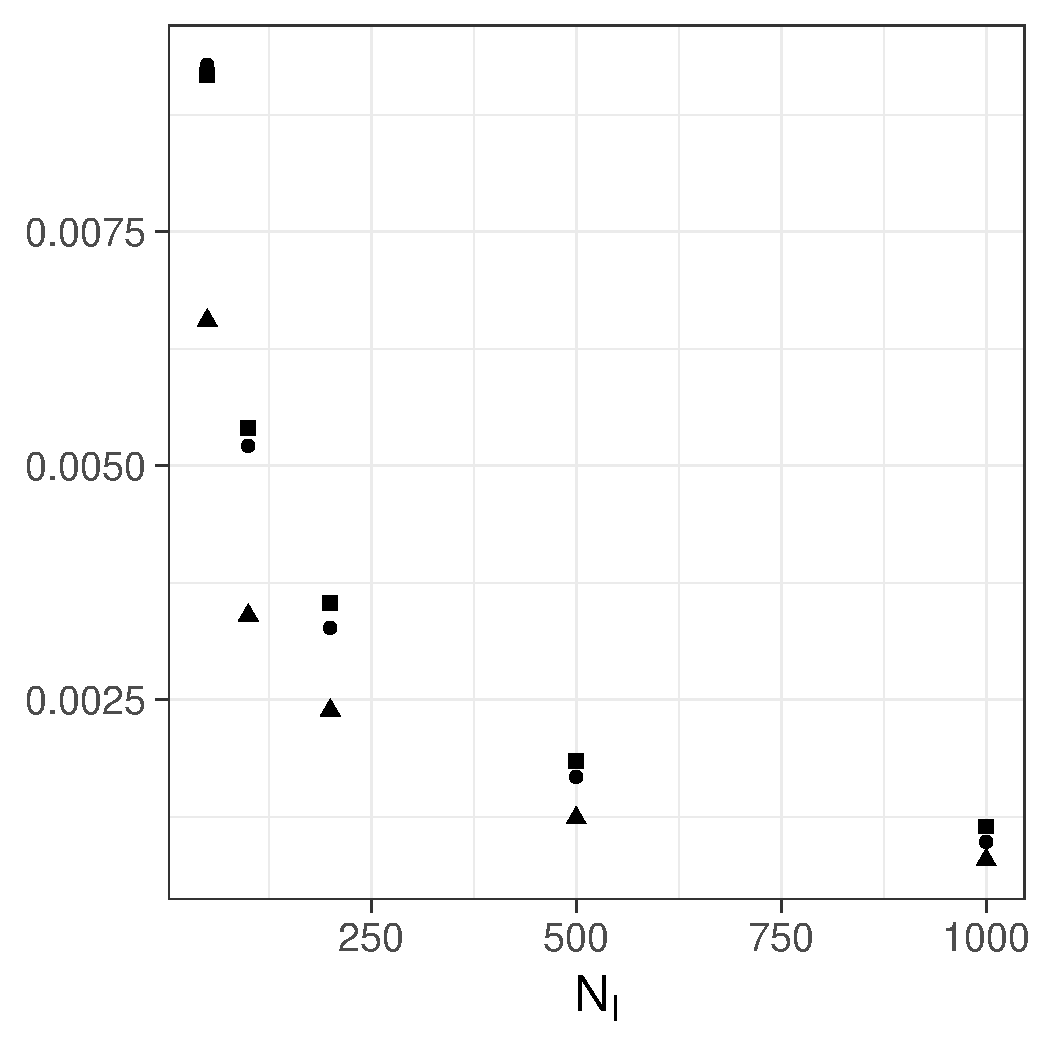
\includegraphics[width=\textwidth]{results/by_pop_size/RMISE-vs-population}
        \caption{\glsentryname{rmise}}
        \label{fig:ise:unifNpop_1h:rmise}
    \end{subfigure}

    \begin{subfigure}[b]{0.49\textwidth}
        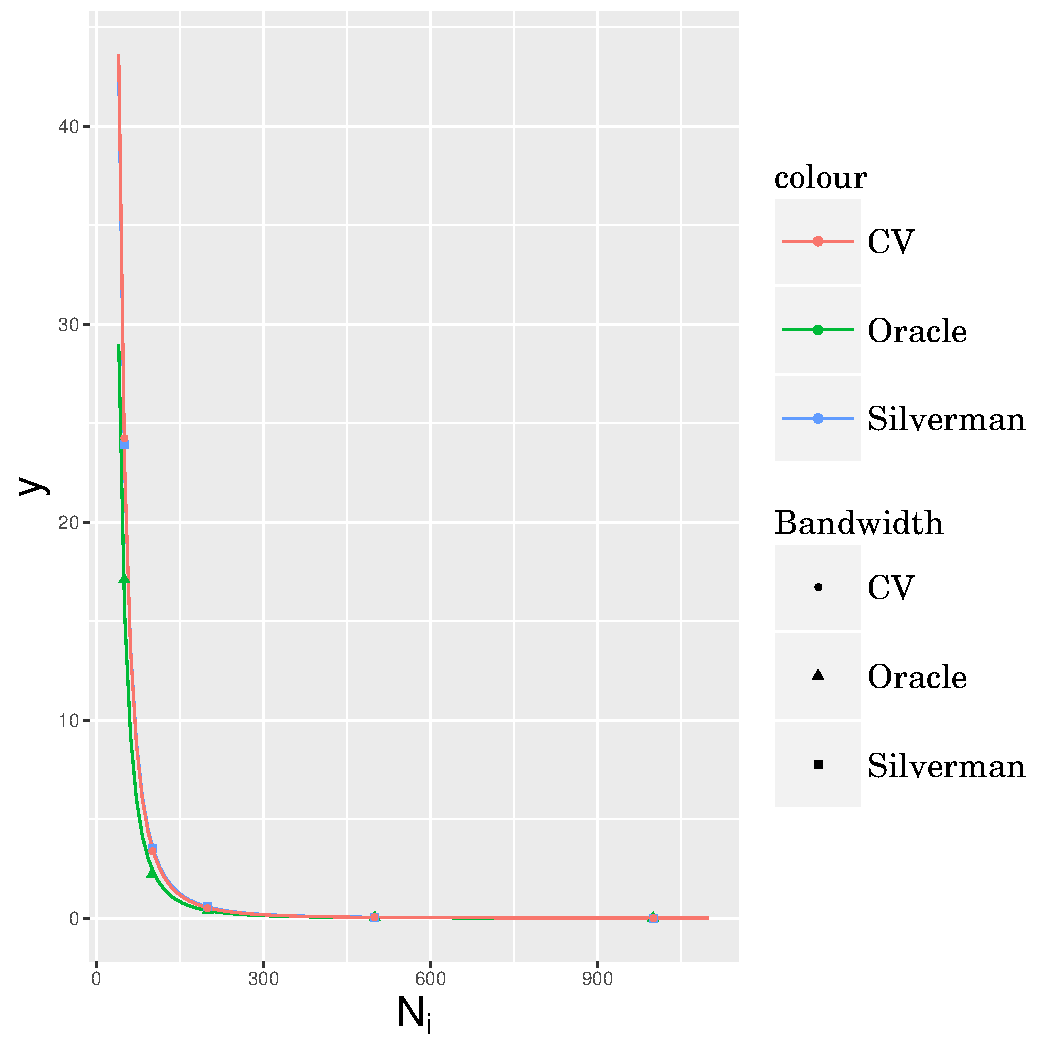
\includegraphics[width=\textwidth]{results/by_pop_size/NMISE-vs-population}
        \caption{\glsentryname{nmise}}
        \label{fig:ise:unifNpop_1h:nmise}
    \end{subfigure}
    \begin{subfigure}[b]{0.49\textwidth}
        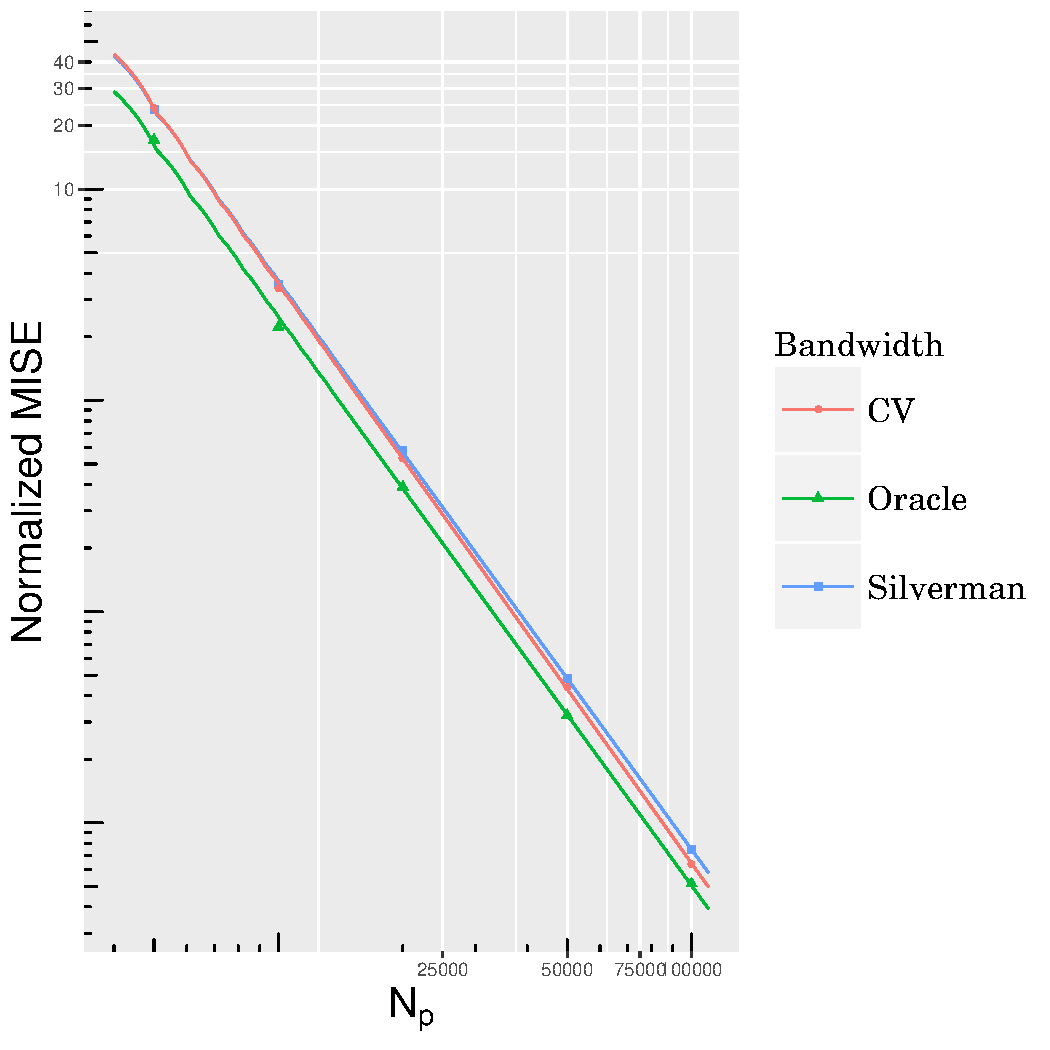
\includegraphics[width=\textwidth]{results/by_pop_size/NMISE-vs-population-log-log}
        \caption{\glsentryname{nmise} log-log}
        \label{fig:ise:unifNpop_1h:nmise_log_log}
    \end{subfigure}
    \caption[\glsentryname{mise}: by sample and population size]{\glsentryname{mise} vs. sample and population size}
    \label{fig:ise:unifNpop_1h}
\end{figure}

In \Cref{fig:ise:unifNpop_1h:mise} we see that in this experiment,
for all bandwidth selections methods the \gls{mise} decreases in a similar manner when the sample and population sizes increase.
\Gls{rmise} also decreases in a similar manner, as shown in \Cref{fig:ise:unifNpop_1h:rmise}.
When we look at \Cref{fig:ise:unifNpop_1h:nmise} we see that the rate of decrease of \gls{nmise} appears to be much higher than \gls{mise}.
In \Cref{tab:results:nmise_convergence_by_sample_size} we see that when we fix the risk function $\lambda \xvec$,
the \gls{nmise} converges at a much higher rate than we observed in \Cref{sec:results:number_of_incidents}.
We also note that selected the bandwidth using \gls{cv} appears to result in a slightly faster rate of convergence than \gls{silverman}.

%latex.default(df.alpha, title = "nmise_convergence_table", where = "htbp",     label = "tab:results:nmise_convergence_by_sample_size", rowname = NULL,     booktabs = TRUE, cdec = c(0, 3), caption.loc = "bottom",     caption = "NMISE convergence rate by sample size for different bandwidth selectors for a fixed, single-peak risk function with expected number of incidents 100 on a uniform population.",     caption.lot = "NMISE Convergence rate by sample size")%
\begin{table}[htbp]
\begin{center}
\begin{tabular}{lr}
\toprule
\multicolumn{1}{c}{Selector}&\multicolumn{1}{c}{Slope}\tabularnewline
\midrule
Oracle&$-2.689$\tabularnewline
Silverman&$-2.688$\tabularnewline
CV&$-2.741$\tabularnewline
\bottomrule
\end{tabular}
\caption[NMISE Convergence rate by sample size]{NMISE convergence rate by sample size for different bandwidth selectors for a fixed, single-peak risk function with expected number of incidents 100 on a uniform population.\label{tab:results:nmise_convergence_by_sample_size}}\end{center}
\end{table}


Regarding the other measures of accuracy, the \gls{miae} and \gls{supremum error} both follow the same pattern as the \gls{mise}:
decreasing as $N_i \to \infty$,
\gls{cv} selected bandwidth producing slightly more accurate \gls{miae} and \glspl{supremum error} than \gls{silverman}.
However, the \gls{peak bias} of the \gls{silverman} bandwidth \glspl{dkd} is still positive, although the \gls{centroid bias} is not.
The \gls{cv} produces much more accurate estimates of \gls{peak drift} than \gls{silverman}, but consistently underestimates the \gls{peak bias} by a greater value.

%%%%%%%%%%%%%%%%%%%%%%%%%%%%%%%%%%%%%%%%%%%%%%%%%%%%%%%%%%%%%%%%%%%%%%%%%%%%%%
%%
%% Section: Varying the spread of the population density
%%
%%%%%%%%%%%%%%%%%%%%%%%%%%%%%%%%%%%%%%%%%%%%%%%%%%%%%%%%%%%%%%%%%%%%%%%%%%%%%%
\section{Varying the spread of the population density}
\label{sec:results:pop_spread}

%%%%%%%%%%%%%%%%%%%%%%%%%%%%%
% Parameter table
%%%%%%%%%%%%%%%%%%%%%%%%%%%%%
\begin{table}[htbp]
    \centering
    \begin{tabular}{ll}
        \toprule
        Parameter & Value \\
        \midrule
        Population size & 10,000 \\
        Population \gls{spread} & 0.7, 1.0, 1.4, 2.0, 2.8 \\
        Population center & (0,0) \\
        \Gls{factor} & 100 \\
        Incident \gls{spread} & 1.0 \\
        Incident center & (0,0) \\
        \bottomrule
    \end{tabular}
    \caption{Parameters used for varying the \glsentryname{spread} of the population peak of 10,000}
    \label{tab:params:pop_spread}
\end{table}

In this section, we compare the effect of different population distributions on the estimation of a single, fixed risk function.
In particular, we vary the \gls{spread} of the population \gls{sigma_p}.
The population size is fixed at 10,000 and centered around the origin (0,0).
We conduct five experiments, using the values 0.7, 1.0, 1.4, 2.0, and 2.8 for \gls{sigma_p}.
An important consideration is that the \gls{factor} \gls{mu} is computed under the assumption of a \textit{uniformly distributed} population.
Since our populations are not uniformly distributed, we expect that the actual number of incidents observed will differ significantly from \gls{mu}.
The results of the experiments described in this section are summarized in \Cref{tab:mean_error_rates:p0.7_100_1.0_1h,tab:mean_error_rates:p1.0_100_1.0_1h,tab:mean_error_rates:p1.4_100_1.0_1h,tab:mean_error_rates:p2.0_100_1.0_1h,tab:mean_error_rates:p2.8_100_1.0_1h}.
An single realization for each of $\gls{sigma_p} = 1.0$ and $\gls{sigma_p} = 2.8$ can be seen in \Cref{fig:one_sample:pop_spread}.
In \subref{fig:one_sample:pop_spread:1.0} we see the population more densely packed into the center.
Consequently there are more incidents,
because the population is greater in the same place that the risk of incidence is higher.

%%%%%%%%%%%%%%%%%%%%%%%%%%%%%%%%%%%%%%%%%%%%%%%%%
% Examples showing population spread
%%%%%%%%%%%%%%%%%%%%%%%%%%%%%%%%%%%%%%%%%%%%%%%%%
\begin{figure}[htbp]
    \centering
    \begin{subfigure}{0.45\textwidth}
        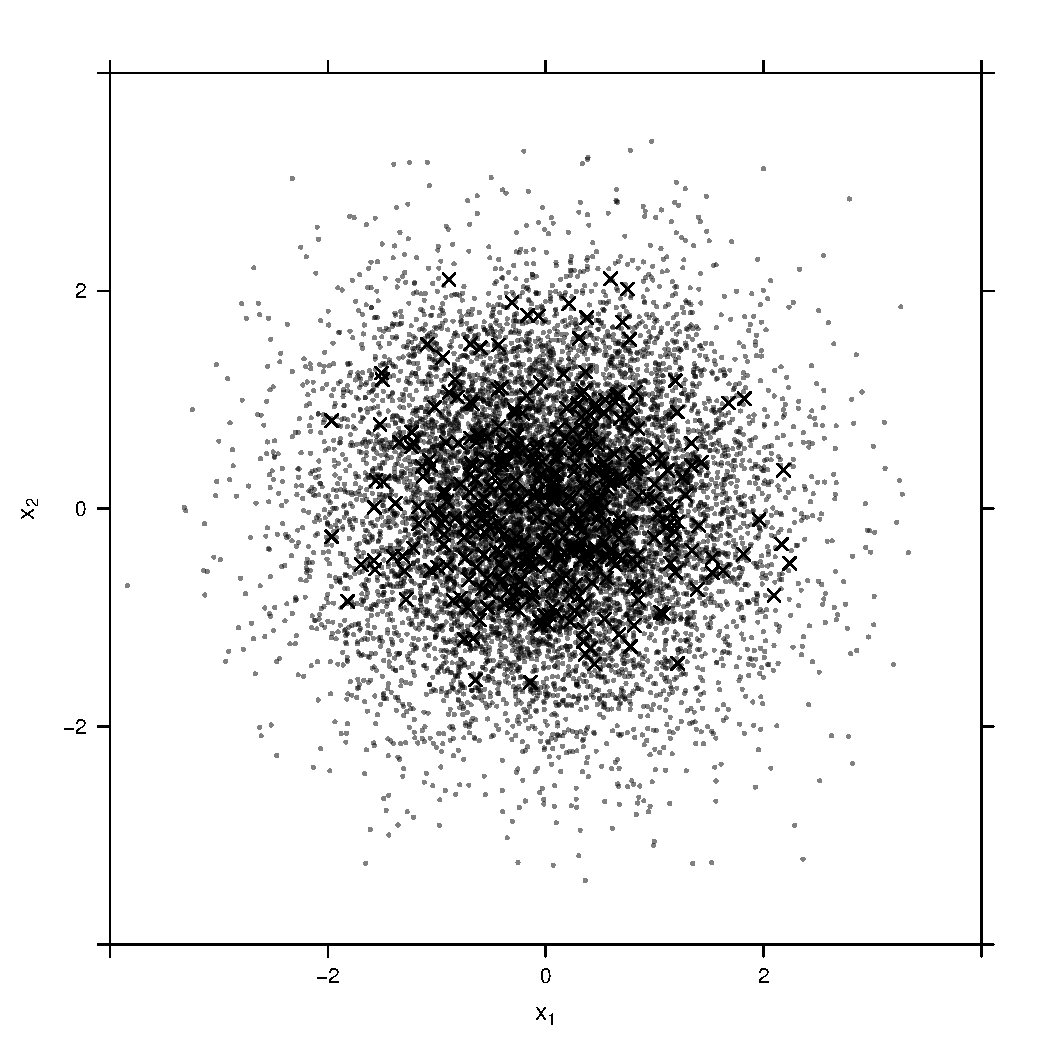
\includegraphics[width=\textwidth]{results/p1.0_100_1.0_1h/output/population_and_incidents_scatter}
        \subcaption{\gls{sigma_p} = 1.0}
        \label{fig:one_sample:pop_spread:1.0}
    \end{subfigure}
    \begin{subfigure}{0.45\textwidth}
        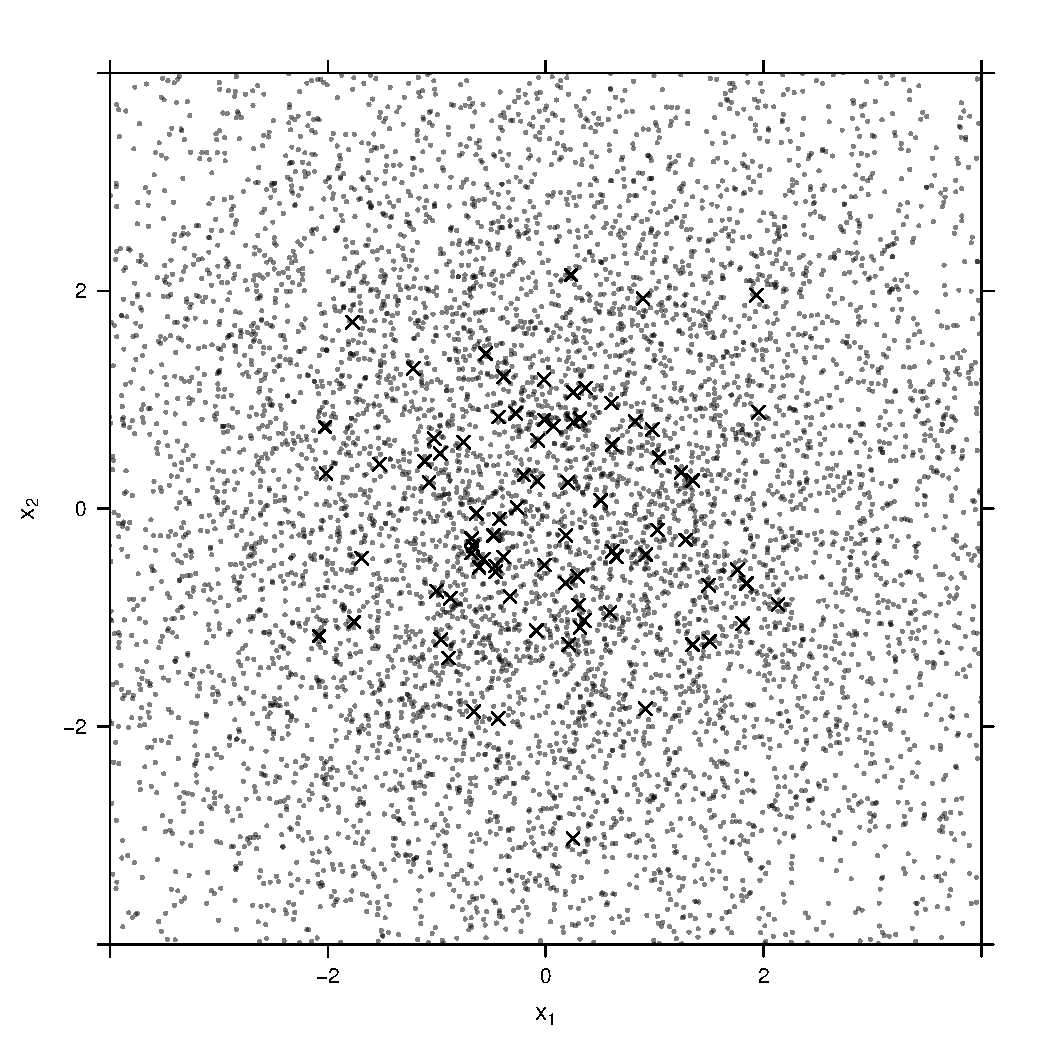
\includegraphics[width=\textwidth]{results/p2.8_100_1.0_1h/output/population_and_incidents_scatter}
        \subcaption{\gls{sigma_p} = 2.8}
        \label{fig:one_sample:pop_spread:2.8}
    \end{subfigure}
    \caption[Examples showing population spread]
        {A single realization of different sample sizes from a single-peak risk on a single-peak population, obtained by varying the population \gls{spread} while keeping population size and the risk function $\lambda \xvec$ fixed.}
    \label{fig:one_sample:pop_spread}
\end{figure}


%%%%%%%%%%%%%%%%%%%%%%%%%%%%%%%%%%%%%%%%%%%%%%%%%
% MISE by population spread
%%%%%%%%%%%%%%%%%%%%%%%%%%%%%%%%%%%%%%%%%%%%%%%%%
\begin{figure}[htbp]
    \centering
    \begin{subfigure}[t]{0.49\textwidth}
        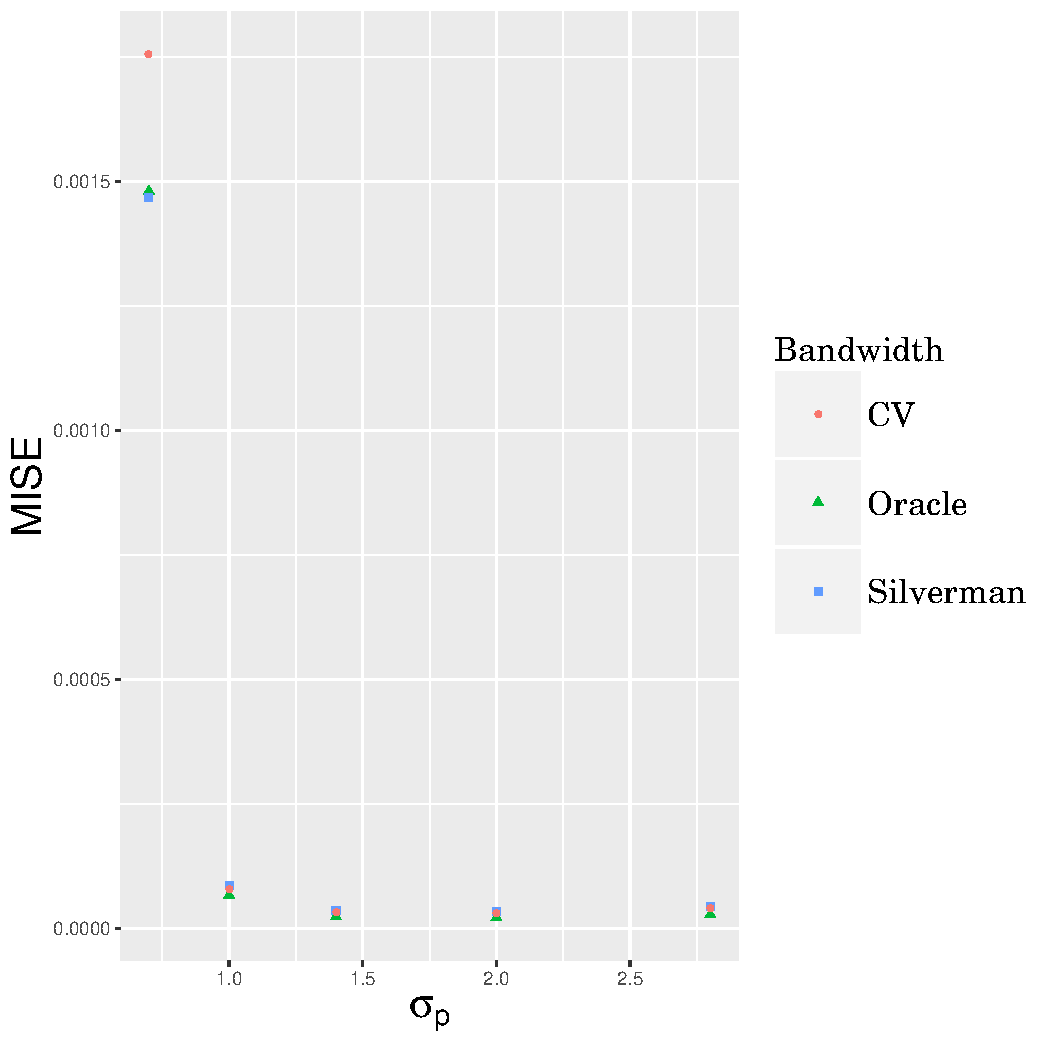
\includegraphics[width=\textwidth]{results/by_population_spread/MISE-vs-population-spread}
        \caption{\glsentryname{mise}}
        \label{fig:ise:pop_spread:mise}
    \end{subfigure}
    \begin{subfigure}[t]{0.49\textwidth}
        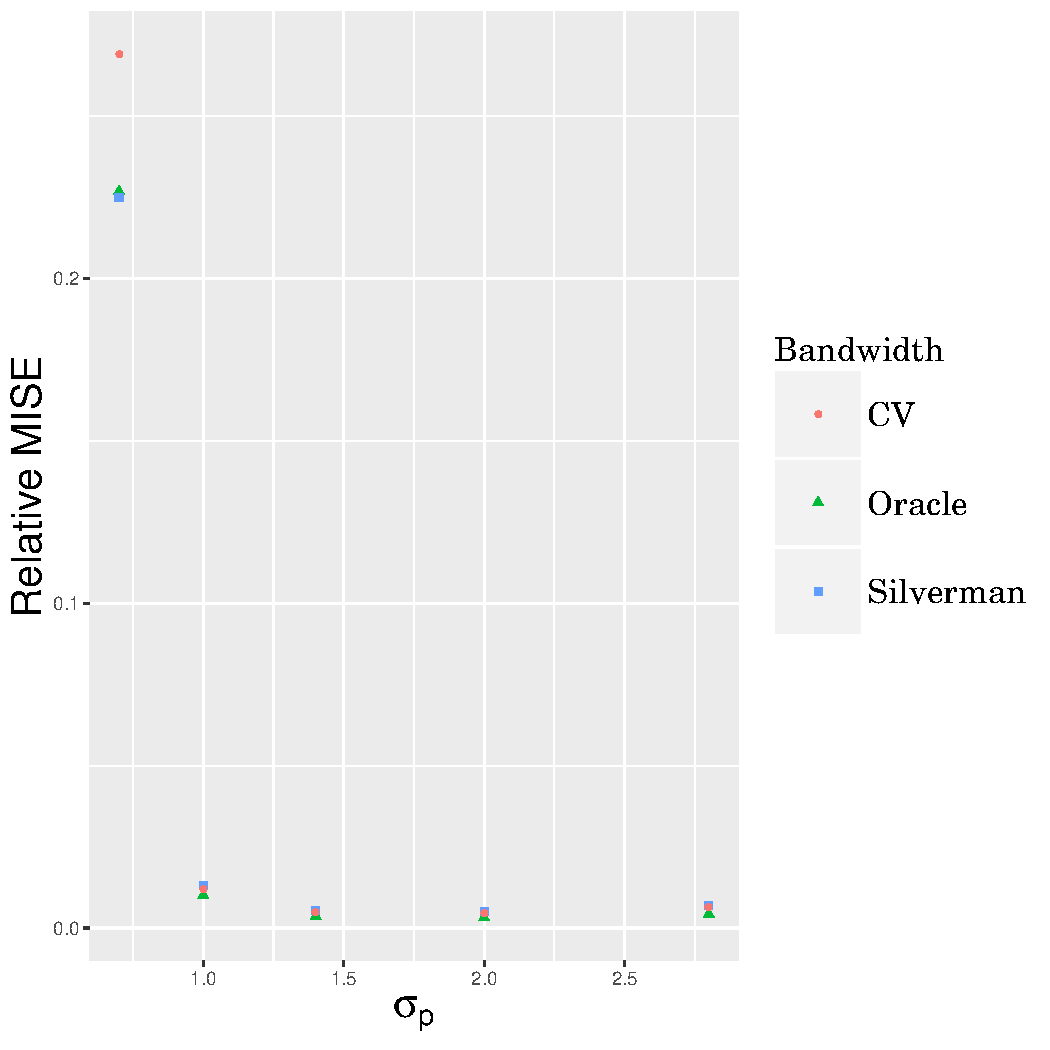
\includegraphics[width=\textwidth]{results/by_population_spread/RMISE-vs-population-spread}
        \caption{\glsentryname{rmise}}
        \label{fig:ise:pop_spread:rmise}
    \end{subfigure}

    \begin{subfigure}[t]{0.49\textwidth}
        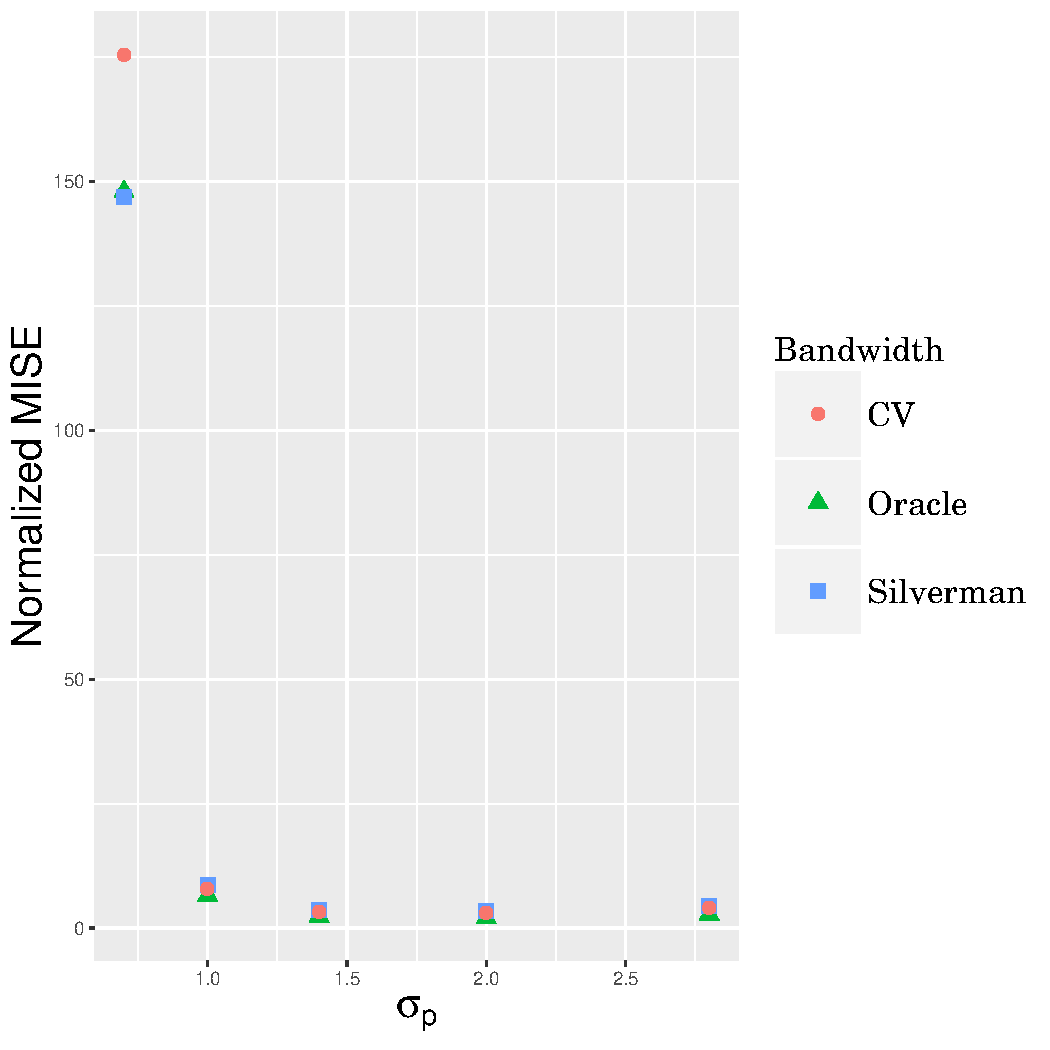
\includegraphics[width=\textwidth]{results/by_population_spread/NMISE-vs-population-spread}
        \caption{\glsentryname{nmise}}
        \label{fig:ise:pop_spread:nmise}
    \end{subfigure}
    \begin{subfigure}[t]{0.49\textwidth}
        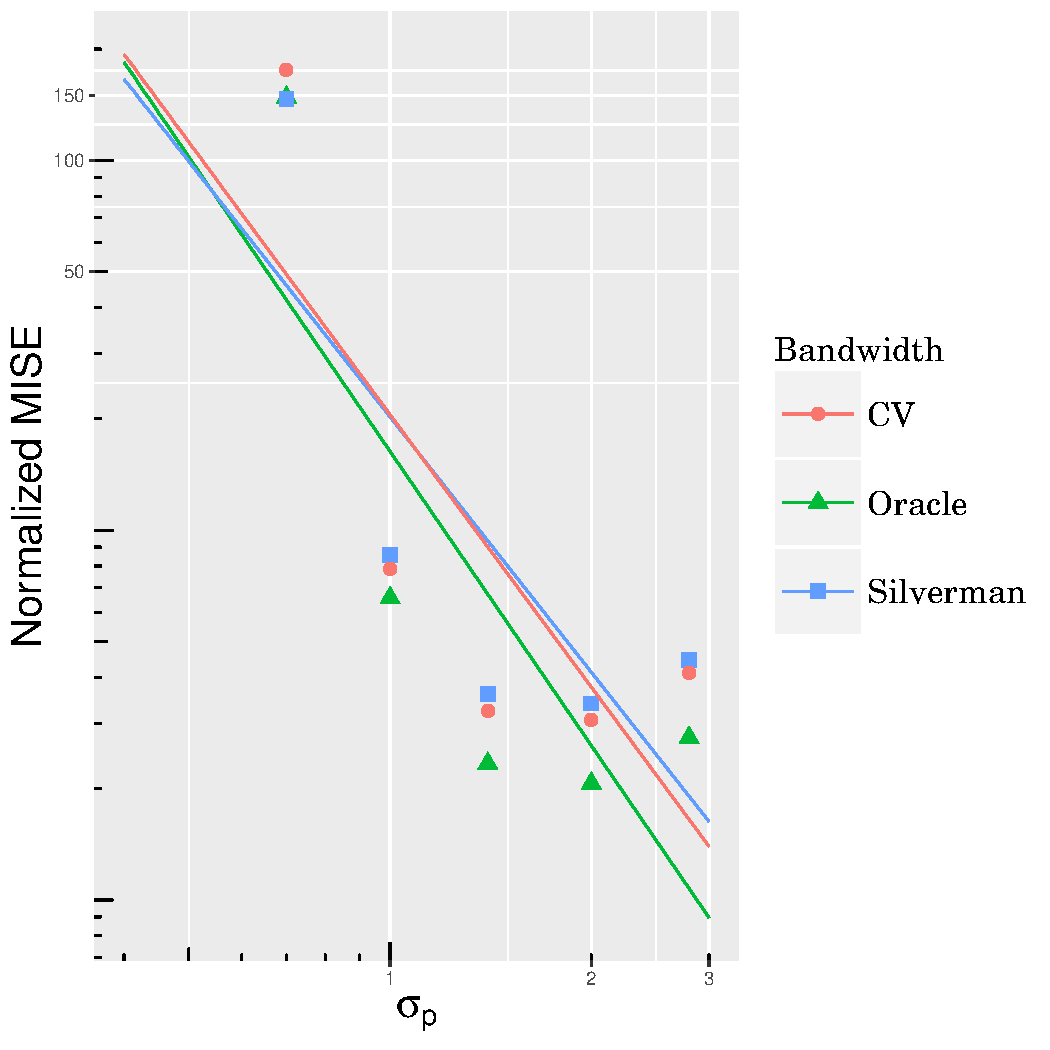
\includegraphics[width=\textwidth]{results/by_population_spread/NMISE-vs-population-spread-log-log}
        \caption{\glsentryname{nmise} log-log}
        \label{fig:ise:pop_spread:nmise_log_log}
    \end{subfigure}
    \caption[\glsentryname{mise}: by population \glsentryname{spread}]{\glsentryname{mise} vs. population \glsentryname{spread}}
    \label{fig:ise:pop_spread}
\end{figure}

\Cref{fig:ise:pop_spread} shows how \gls{mise}, \gls{rmise} and \gls{nmise} are affected by population spread.
In \subref{fig:ise:pop_spread:nmise_log_log} it does not appear that there is any linear relationship,
and there does not appear to be any convergence to zero of any of these measures as $\gls{sigma_p} \to \infty$.
In fact, it appears that as long as the population distribution does not change too rapidly,
the \gls{dkd} gives similar performance for any population \gls{spread}.

Regarding the other accuracy measures, we see that \gls{miae} and \gls{supremum error} are similar,
in that for $\gls{sigma_p} = 0.7$ the values are very high,
but they are generally low for other values of \gls{sigma_p}.
Because the risk function $\gls{lambda} \xvec$ is identical across experiments,
the relative, normal and absolute measures all have similar patterns
as seen in \Cref{fig:other_measures:pop_spread}.

%%%%%%%%%%%%%%%%%%%%%%%%%%%%%%%%%%%%%%%%%%%%%%%%%
% Other accuracy measures by population spread
%%%%%%%%%%%%%%%%%%%%%%%%%%%%%%%%%%%%%%%%%%%%%%%%%
\begin{figure}[htbp]
    \centering
    \begin{subfigure}[t]{0.49\textwidth}
        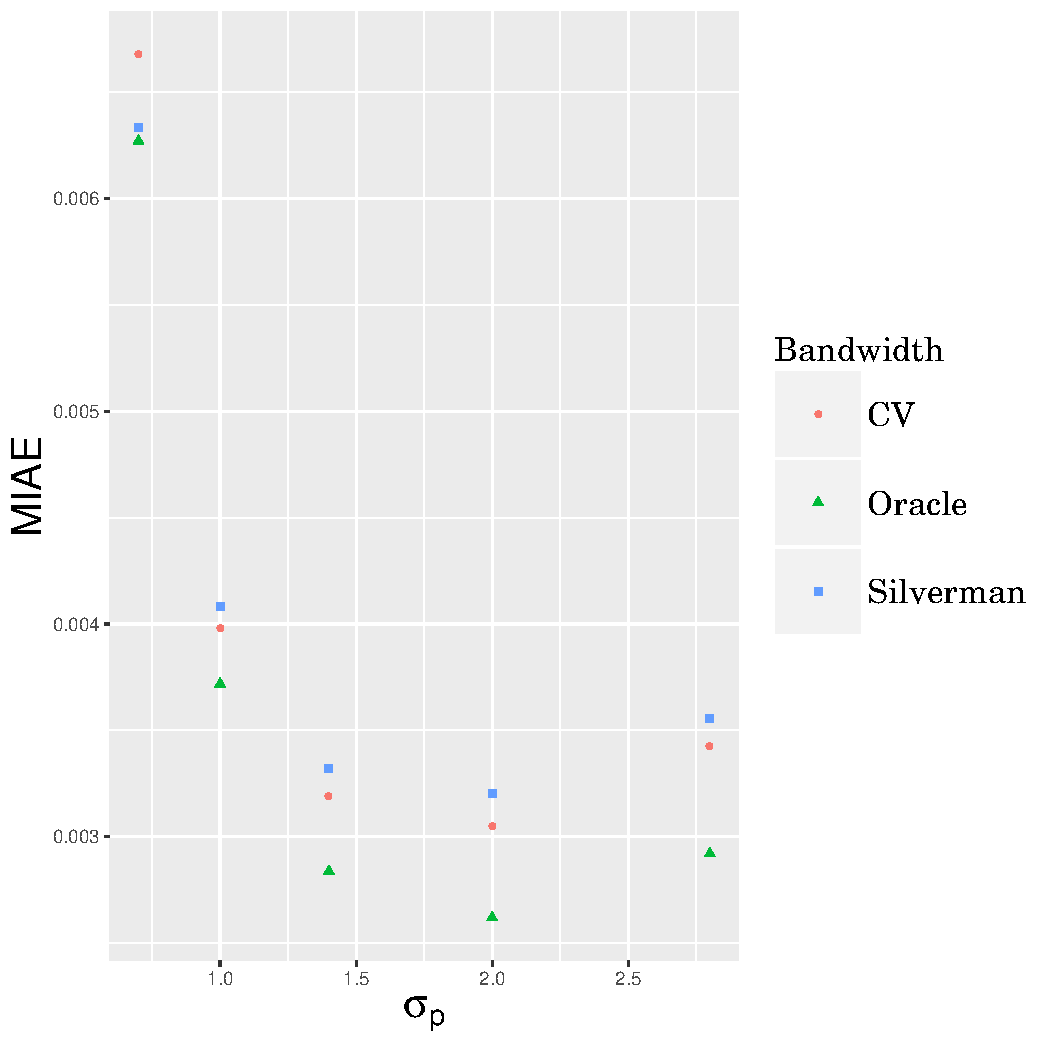
\includegraphics[width=\textwidth]{results/by_population_spread/MIAE-vs-population-spread}
        \subcaption{\glsentryname{miae}}
        \label{fig:other_measures:pop_spread:miae}
    \end{subfigure}
    \begin{subfigure}[t]{0.49\textwidth}
        \includegraphics[width=\textwidth]{results/by_population_spread/maxerr-vs-population-spread}
        \subcaption{\Glsentryname{supremum error}}
        \label{fig:other_measures:pop_spread:maxerr}
    \end{subfigure}
    \caption{\glsentryname{miae} and \Glsentryname{supremum error} by population \glsentryname{spread}}
    \label{fig:other_measures:pop_spread}
\end{figure}

%%%%%%%%%%%%%%%%%%%%%%%%%%%%%%%%%%%%%%%%%%%%%%%%%%%%%%%%%%%%%%%%%%%%%%%%%%%%%%
%%
%% Section: Distance between two peaks
%%
%%%%%%%%%%%%%%%%%%%%%%%%%%%%%%%%%%%%%%%%%%%%%%%%%%%%%%%%%%%%%%%%%%%%%%%%%%%%%%
\section{Distance between two peaks}
\label{sec:results:p1.4_100_G}

%%%%%%%%%%%%%%%%%%%%%%%%%%%%%
% Parameter table
%%%%%%%%%%%%%%%%%%%%%%%%%%%%%
\begin{table}[htbp]
    \centering
    \begin{tabular}{ll}
        \toprule
        Parameter & Value \\
        \midrule
        Population size & 10,000 \\
        Population \gls{spread} & uniform \\
        Population center & uniform \\
        \Gls{factor} & 40, 60 \\
        Incident \gls{spread} & 1.0 \\
        Incident center & \{(0.5,0), (-0.5,0)\},  \{(1,0), (-1,0)\}, \{(1.5,0), (-1.5,0)\}, \{(2,0), (-2,0)\}\\
        \bottomrule
    \end{tabular}
    \caption{Parameters used for varying the two peaks of the risk function with \glspl{factor} 40 and 60 on a uniform population of 10,000}
    \label{tab:params:p1.4_100_G}
\end{table}

In this section, we look at incident risk functions that have two peaks.
The major peak has a \gls{factor} of 60, while the second, minor peak has a \gls{factor} of 40.
We do this to see how the minor peak affects the accuracy of the measuring the \gls{dkd} in general and the \gls{peak bias} and \gls{peak drift} in particular.
The results of the experiments described in this section are summarized in \Cref{tab:mean_error_rates:unif_100_1_2h_1,tab:mean_error_rates:unif_100_1_2h_2,tab:mean_error_rates:unif_100_1_2h_3,tab:mean_error_rates:unif_100_1_2h_4}.

%%%%%%%%%%%%%%%%%%%%%%%%%%%%%%%%%%%%%%%%%%%%%%%%%
% Examples showing distance between two peaks
%%%%%%%%%%%%%%%%%%%%%%%%%%%%%%%%%%%%%%%%%%%%%%%%%
\begin{figure}[htbp]
    \centering
    \begin{subfigure}{0.45\textwidth}
        \includegraphics[width=\textwidth]{results/unif_100_1_2h_2/output/population_and_incidents_scatter}
        \subcaption{Centers at $\{(1,0), (-1,0)\}$ (distance 2)}
        \label{fig:one_sample:p1.4_100_G:2}
    \end{subfigure}
    \begin{subfigure}{0.45\textwidth}
        \includegraphics[width=\textwidth]{results/unif_100_1_2h_4/output/population_and_incidents_scatter}
        \subcaption{Centers at $\{(2,0), (-2,0)\}$ (distance 4)}
        \label{fig:one_sample:p1.4_100_G:4}
    \end{subfigure}
    \caption[Examples showing distance between two peaks]
        {A single realization of different sample sizes from a double-peak risk on a uniform population, obtained by varying the distance between two peaks in the incident risk function.}
    \label{fig:one_sample:p1.4_100_G}
\end{figure}


%%%%%%%%%%%%%%%%%%%%%%%%%%%%%%%%%%%%%%%%%%%%%%%%%
% MISE by peak distance
%%%%%%%%%%%%%%%%%%%%%%%%%%%%%%%%%%%%%%%%%%%%%%%%%
\begin{figure}[htbp]
    \centering
    \begin{subfigure}[b]{0.49\textwidth}
        \includegraphics[width=\textwidth]{results/by_two_peaks/MISE-vs-risk-peak-gap}
        \caption{\glsentryname{mise}}
    \end{subfigure}

    \begin{subfigure}[b]{0.49\textwidth}
        \includegraphics[width=\textwidth]{results/by_two_peaks/RMISE-vs-risk-peak-gap}
        \caption{\glsentryname{rmise}}
    \end{subfigure}
    \begin{subfigure}[b]{0.49\textwidth}
        \includegraphics[width=\textwidth]{results/by_two_peaks/NMISE-vs-risk-peak-gap}
        \caption{\glsentryname{nmise}}
    \end{subfigure}
    \caption{\glsentryname{mise} by distance between two risk peaks}
    \label{fig:ise:p1.4_100_G}
\end{figure}

%%%%%%%%%%%%%%%%%%%%%%%%%%%%%%%%%%%%%%%%%%%%%%%%%
% Other measures by peak distance
%%%%%%%%%%%%%%%%%%%%%%%%%%%%%%%%%%%%%%%%%%%%%%%%%
\begin{figure}[htbp]
    \centering
    \begin{subfigure}[b]{0.49\textwidth}
        \includegraphics[width=\textwidth]{results/by_two_peaks/peak-bias-vs-risk-peak-gap}
        \caption{\glsentryname{peak bias}}
        \label{fig:other_measures:p1.4_100_G:peak_bias}
    \end{subfigure}
    \begin{subfigure}[b]{0.49\textwidth}
        \includegraphics[width=\textwidth]{results/by_two_peaks/peak-drift-vs-risk-peak-gap}
        \caption{\glsentryname{peak drift}}
        \label{fig:other_measures:p1.4_100_G:peak_drift}
    \end{subfigure}

    \begin{subfigure}[b]{0.49\textwidth}
        \includegraphics[width=\textwidth]{results/by_two_peaks/centroid-bias-vs-risk-peak-gap}
        \caption{\glsentryname{centroid bias}}
        \label{fig:other_measures:p1.4_100_G:centroid_bias}
    \end{subfigure}
    \begin{subfigure}[b]{0.49\textwidth}
        \includegraphics[width=\textwidth]{results/by_two_peaks/centroid-drift-vs-risk-peak-gap}
        \caption{\glsentryname{centroid drift}}
        \label{fig:other_measures:p1.4_100_G:centroid_drift}
    \end{subfigure}
    \caption{Other accuracy measures by distance between two risk peaks}
    \label{fig:other_measures:p1.4_100_G}
\end{figure}

We observe that \gls{mise}, \gls{rmise} and \gls{nmise} all increase when the distance between two peaks increases (\Cref{fig:ise:p1.4_100_G}).
The \gls{peak drift} and \gls{centroid drift} also increase when the distance between the two peaks increases (\Cref{fig:other_measures:p1.4_100_G:peak_drift,fig:other_measures:p1.4_100_G:centroid_drift}).
However, we also observe that \gls{peak bias} and \gls{centroid bias} decrease as the distance between the two peaks increases (\Cref{fig:other_measures:p1.4_100_G:peak_bias,fig:other_measures:p1.4_100_G:centroid_bias}).


%%%%%%%%%%%%%%%%%%%%%%%%%%%%%%%%%%%%%%%%%%%%%%%%%%%%%%%%%%%%%%%%%%%%%%%%%%%%%%
%%
%% Section: Distance between the population and risk function peaks
%%
%%%%%%%%%%%%%%%%%%%%%%%%%%%%%%%%%%%%%%%%%%%%%%%%%%%%%%%%%%%%%%%%%%%%%%%%%%%%%%
\section{Distance between the population and risk function peaks}
\label{sec:results:p1.4_Gap_risk}

%%%%%%%%%%%%%%%%%%%%%%%%%%%%%
% Parameter table
%%%%%%%%%%%%%%%%%%%%%%%%%%%%%
\begin{table}[htbp]
    \centering
    \begin{tabular}{ll}
        \toprule
        Parameter & Value \\
        \midrule
        Population size & 10,000 \\
        Population \gls{spread} & 1.4 \\
        Population center & (-0.5,0), (-1,0), (-1.5,0), (-2,0) \\
        \Gls{factor} & 40, 60 \\
        Incident \gls{spread} & 1.0 \\
        Incident center & (0.5,0), (1,0), (1.5,0), (2,0) \\
        \bottomrule
    \end{tabular}
    \caption{Parameters used for varying the peak of the single-peak risk function with \glspl{factor} 100 and the peak of the single-peak population of 10,000}
    \label{tab:params:p1.4_100_Gap_risk}
\end{table}

In this section, we look at incident risk function that have their peak at a different location from the peak in the population distribution.
We expect that as this distance grows, the relatively small population at the peak of the incident risk will make it difficult to obtain any information through observing incidents and estimating with the \gls{dkd}.
The results of the experiments described in this section are summarized in \Cref{tab:mean_error_rates:p1.4_100_1_1h_1s,tab:mean_error_rates:p1.4_100_1_1h_2s,tab:mean_error_rates:p1.4_100_1_1h_3s,tab:mean_error_rates:p1.4_100_1_1h_4s}.

%%%%%%%%%%%%%%%%%%%%%%%%%%%%%%%%%%%%%%%%%%%%%%%%%
% Examples showing distance between population
% and incident peaks
%%%%%%%%%%%%%%%%%%%%%%%%%%%%%%%%%%%%%%%%%%%%%%%%%
\begin{figure}[htbp]
    \centering
    \begin{subfigure}{0.45\textwidth}
        \includegraphics[width=\textwidth]{results/p1.4_100_1_1h_2s/output/population_and_incidents_scatter}
        \subcaption{Centers at $\{(-1,0), (1,0)\}$ (distance 2)}
        \label{fig:one_sample:p1.4_100_Gap_risk:2}
    \end{subfigure}
    \begin{subfigure}{0.45\textwidth}
        \includegraphics[width=\textwidth]{results/p1.4_100_1_1h_4s/output/population_and_incidents_scatter}
        \subcaption{Centers at $\{(-2,0), (2,0)\}$ (distance 4)}
        \label{fig:one_sample:p1.4_100_Gap_risk:4}
    \end{subfigure}
    \caption[Examples showing distance between population and incident peaks]
        {A single realization of different sample sizes from a single-peak risk on a single-peak population, obtained by varying the distance between two peaks.}
    \label{fig:one_sample:p1.4_100_Gap_risk}
\end{figure}

%%%%%%%%%%%%%%%%%%%%%%%%%%%%%%%%%%%%%%%%%%%%%%%%%
% MISE by distance between population
% and incident peaks
%%%%%%%%%%%%%%%%%%%%%%%%%%%%%%%%%%%%%%%%%%%%%%%%%
\begin{figure}[htbp]
    \centering
    \begin{subfigure}[b]{0.49\textwidth}
        \includegraphics[width=\textwidth]{results/by_pop_risk_distance/MISE-vs-population-risk-gap}
        \caption{\glsentryname{mise}}
        \label{fig:ise:p1.4_100_Gap_risk:mise}
    \end{subfigure}
    \begin{subfigure}[b]{0.49\textwidth}
        \includegraphics[width=\textwidth]{results/by_pop_risk_distance/RMISE-vs-population-risk-gap}
        \caption{\glsentryname{rmise}}
        \label{fig:ise:p1.4_100_Gap_risk:rmise}
    \end{subfigure}

    \begin{subfigure}[b]{0.49\textwidth}
        \includegraphics[width=\textwidth]{results/by_pop_risk_distance/NMISE-vs-population-risk-gap}
        \caption{\glsentryname{nmise}}
        \label{fig:ise:p1.4_100_Gap_risk:nmise}
    \end{subfigure}
    \begin{subfigure}[b]{0.49\textwidth}
        \includegraphics[width=\textwidth]{results/by_pop_risk_distance/NMISE-vs-population-risk-gap-log-log}
        \caption{Log-log of \glsentryname{nmise}}
        \label{fig:ise:p1.4_100_Gap_risk:nmise_log_log}
    \end{subfigure}    
    \caption{\glsentryname{mise} by distance between two risk peaks}
    \label{fig:ise:p1.4_100_Gap_risk}
\end{figure}

%latex.default(df.alpha, title = "nmise_convergence_table", where = "htbp",     label = "tab:results:nmise_convergence_by_pop_incident_gap",     rowname = NULL, booktabs = TRUE, cdec = c(0, 3), caption.loc = "bottom",     caption = "NMISE convergence rate by incident-population peak distance for different bandwidth selectors for a single-peak risk function with spread of 1.0 on a single-peak population of 10,000.",     caption.lot = "NMISE Convergence rate by incident-population peak distance")%
\begin{table}[htbp]
\begin{center}
\begin{tabular}{lr}
\toprule
\multicolumn{1}{c}{Selector}&\multicolumn{1}{c}{Gap}\tabularnewline
\midrule
Oracle&$1.110$\tabularnewline
Silverman&$1.055$\tabularnewline
CV&$1.181$\tabularnewline
\bottomrule
\end{tabular}
\caption[NMISE Convergence rate by incident-population peak distance]{NMISE convergence rate by incident-population peak distance for different bandwidth selectors for a single-peak risk function with spread of 1.0 on a single-peak population of 10,000.\label{tab:results:nmise_convergence_by_pop_incident_gap}}\end{center}
\end{table}


\Cref{fig:ise:p1.4_100_Gap_risk} shows the different measures of \gls{mise} accuracy.
We can see from \Cref{fig:ise:p1.4_100_Gap_risk:nmise_log_log} that there is a linear relationship in the log-log graph,
indicating polynomial increase with positive coefficient of \gls{mise} when the distance between the incident and population peaks increases.
We see in \Cref{tab:results:nmise_convergence_by_pop_incident_gap} that the exponent is just over 1,
indicating just worse than linear.

% ensure the path is set back
\setpath{}
